\chapter{Sleep stage classification}\label{chap:sleep-stage-classification}
% \acresetall
\begin{flushright}{
        \texttt{What is my purpose?}\\{\slshape You pass butter.}\\\texttt{Oh my God.}} \\ \medskip
        --- Butter Robot to Rick Sanchez\\Rick and Morty, season 1, episode 9
\end{flushright}
\vspace{6cm}

This chapter presents methods and main findings in two published research papers and one manuscript currently under review regarding automatic methods for sleep stage classification.

First, the problem of automated sleep stage classification is presented and associated research questions are formulated. 
Then, an initial version of the \acf{MASSC} model based on end-to-end deep learning is presented along with the results published in~\cite{Olesen2018c}, which is followed by the findings from applying an updated version of the model in a multi-cohort experimental setting.
Afterwards, the \ac{STAGES} model for sleep stage classification originally published in~\cite{Stephansen2018} is presented along with results compared to multiple scorers.
The chapter will conclude with a summary of the main findings in~\cref{sec:sleep-stage-classification:summary}

Parts of this chapter have been modified from their original publications. 
\begin{itemize}
    \item \Cref{sec:paperi} has been modified from \newline \printpublication{Olesen2018c}\footnote{\textcopyright 2018 IEEE}.
    \item \Cref{sec:paperii} is based on \newline \printpublication{Olesen2020AutomaticSetting}.
    \item \Cref{sec:paperiii} has been modified from \newline \printpublication{Stephansen2018}\footnote{Creative Commons Attributes 4.0 International License: \url{http://creativecommons.org/licenses/by/4.0/}}.
\end{itemize} 

\section{Research background}

% Sleep staging is the principal tool available to medical doctors in the analysis of sleep disorders. 
% Natural human sleep consists of recurring cycles of three to four distinct phases, which are primarily characterized by changes in brain activity, eye movements, muscle activations and breathing.
% A \ac{PSG} containing \ac{EEG}, \ac{EOG}, \ac{EMG} and other bioelectric signals is collected during sleep, and subsequently processed and analyzed by sleep technicians according to standards by the \ac{AASM}. 
% Each \SI{30}{\second} epoch of data is categorized into either \ac{W}, \ac{REM} sleep, or one of three stages of non-\ac{REM} sleep (\ac{N1}, \ac{N2},\ac{N3})~\cite{Berry2016}. 
% However, this approach is prone to subjective interpretation of sleep staging rules, which have prompted extensive research in using various signal processing and machine learning approaches~\cite{Sen2014}.

Sleep staging is important to the analysis of human sleep with about \num{845000} sleep studies performed in 2014 in the US alone~\cite{Chiao2017}. 
A standard clinical sleep study consists of a full-night \ac{PSG} comprising \ac{EEG}, \ac{EOG}, \ac{EMG}, \ac{ECG}, respiratory inductance plethysmography, oronasal thermal flow, nasal pressure, and blood oxygen saturation recordings.
These studies are evaluated by experts for the presence of events of clinical relevance, as determined by standards created by the \ac{AASM}, such as the number of blood oxygen desaturations, micro-arousals, leg movements, periods of cessated breathing, to name a few. 
The overall sleep architecture is captured in a visual representation called a hypnogram, which is achieved by labeling every \SI{30}{\second} of \ac{PSG} data into one of five stages of sleep: \ac{W}, \ac{REM} sleep, \ac{N1}, \ac{N2}, and \ac{N3}, and plotting as a function of time. 
The latter three stages are distinguished by distinct \ac{EEG} amplitude and frequency distributions, the presence of specific \ac{EEG} micro-events and arousability differences reflecting sleep depth.

Sleep stage scoring is summarized in key metrics, such as the percentage of \ac{TST} spent in any of the five stages (\%\ac{W}, or \ac{WASO}; \%\ac{REM}; \%\ac{N1}; \%\ac{N2}; \%\ac{N3}), and visually in the form of a hypnogram, which shows temporal progression of sleep stages across the night as mentioned. 
Current clinical practice (gold standard) of sleep study analysis is manual scoring and annotation of sleep stages and sleep events based on guidelines from the \ac{AASM}~\cite{Berry2018}. 
\graffito{This is described in detail in~\cref{sec:challenges-sleep-stage-scoring}}These guidelines, based on observations made in healthy young males almost 70 years ago, are problematic for several reasons: a) technicians will never score the same data the exact same way as another technician, or even the same way twice~\cite{Norman2000,Rosenberg2013,Younes2016,Younes2017,Younes2018}; b) normal sleep from healthy young males may not reflect sleep patterns of patients referred to sleep clinics; and c) the \SI{30}{\second} epoch rule was arbitrarily based on physical limitations of recording equipment, when \acp{PSG} were recorded on paper, and may not accurately reflect the true underlying neurobiological mechanisms.

Automatic sleep stage classification has not yet seen wide-spread adoption in clinical practice despite ongoing research demonstrating feasibility and industrial interests~\cite{Fiorillo2019}. 
A major issue has been a lack of available data for designing and training models. 
The publicly available PhysioNet Sleep-EDF and the expanded version databases~\cite{Goldberger2000,Kemp2000} has been used extensively for training both shallow and deep learning-based machine learning models~\cite{Vilamala2017,Phan2018,Supratak2017}, but given the small sample size and homogeneity (most papers use the same healthy 20 subjects), it is questionable how well models derived from this data generalize to unseen data, even if high classification performance is often reported~\cite{Fiorillo2019}. 
Other databases which have been extensively used include the St. Vincent’s University Hospital and University College Dublin Sleep Apnea Database (\(n=25\))~\cite{Goldberger2000,Sen2014}, and the Montreal Archive of Sleep Studies (MASS, \(n=200\))~\cite{OReilly2014,Supratak2017,Chambon2018c,Andreotti2018,Phan2019a,Phan2019b}. 

The argument for using deep learning-based models to classify high-dimensional electrophysiological data, e.g. \acp{PSG}, into discrete outcomes such as sleep stages is compelling, because of their ability to capture variability in the underlying highly complex data representations, that might be missed by machine learning methods relying on manual feature engineering.
In the image, speech, and natural language processing domains, the success of deep learning models using un-transformed data has been unsurpassed in the last decade, thanks largely due to the availability of ever-increasing amounts of compute resources and more significantly very large, robust and diverse datasets~\cite{LeCun2015}.

Recently deep learning models for automatic sleep stage classification have been developed and validated using two or more databases or cohorts~\cite{Stephansen2018, Biswal2018, Patanaik2018}, or a single large volume cohort~\cite{Biswal2018, Olesen2018c,Biswal2017}. 
The assumption has been that by incorporating multiple sources of variance in the dataset used for training (\eg from multiple technicians, sites, recording setups, equipment, \etc), final models will be better at generalizing to new, unseen data. 
However, no study to date has investigated multiple, large-scale cohorts for automatic sleep stage classification, or how different cohorts generalize to one another.

\subsection{Research motivation and objectives}

Motivated by these issues, we were interested in the following research questions specifically related to research hypothesis~\ref{hypothesis:sleep-stages}\graffito{\ref{hypothesis:sleep-stages}: \hypothesis\xspace sleep stages.}:
\newcommand{\questionSleepStageClassification}{can sleep stages be effectively and reliably classified using novel machine learning algorithms}
\newcommand{\questionSleepStageDatasets}{in cases of multiple available data sources, is it better to have more volume or more diverse data}
\newcommand{\questionSleepStageGuarantee}{how can we guarantee that such a system is stable with respect to the impact of sleep disorders}
\begin{enumerate}[label={\footnotesize\bfseries\scshape RQ~1.\arabic*}, ref={\bfseries\scshape RQ~1.\arabic*}]
    \item \questionSleepStageClassification\label{question:sleep-stages-classification},
    \item \questionSleepStageDatasets\label{question:sleep-stages-datasets},
    \item \questionSleepStageGuarantee\label{question:sleep-stages-guarantee}.
\end{enumerate}

Derived from the research hypothesis and associated questions, the following research objectives were formulated:

\begin{enumerate}[label=(\roman*)]
    \item a single model should classify sleep stages and assign probabilities to each sleep stage to allow for stage mixing;
    \item the model should be tested using as diverse data as possible.
\end{enumerate}

The following sections describe the steps taken to complete the research objectives and answer the research questions.


% Research papers
\clearpage\section{Paper I: Deep residual networks for automatic sleep stage classification of raw polysomnographic waveforms}\label{sec:paperi}
\sectionmark{Olesen, Jennum, Peppard, Sorensen, \& Mignot, 2018}

% \begin{tcolorbox}[colframe=dtu-red!50, colback=white]
\begin{tcolorbox}[colframe=white]
\paragraph{Abstract} We have developed an automatic sleep stage classification algorithm based on deep residual neural networks and raw polysomnogram signals. 
Briefly, the raw data is passed through 50 convolutional layers before subsequent classification into one of five sleep stages. 
Three model configurations were trained on 1850 polysomnogram recordings and subsequently tested on 230 independent recordings. 
Our best performing model yielded an accuracy of 84.1\% and a Cohen's kappa of 0.746, improving on previous reported results by other groups also using only raw polysomnogram data. 
Most errors were made on non-REM stage 1 and 3 decisions, errors likely resulting from the definition of these stages. 
Further testing on independent cohorts is needed to verify performance for clinical use.
\end{tcolorbox}

\subsection{Methods}
\subsubsection{Data}
A database containing 2310 recordings extracted from the \ac{WSC} was used in this study.
Specific acquisition details concerning the \acp{PSG} are described in~\cite{Young1993,Young2008}.
The entire set of \ac{PSG} studies was randomly split into training (train), validation (eval), and testing (test) subgroups in an 8:1:1 ratio.
Detailed demographic information as well as relevant \ac{PSG} variables for all three subgroups are provided in~\cref{tab:sleep-stages:wsc_demographics} including \ac{AHI} and time spent in each sleep stage based on manual scoring. %No statistically significant differences between subgroups were found except for the amount of N1 and N2 sleep.

\subsubsection{Data processing pipeline}
Central and occipital \ac{EEG} from the right hemisphere, left and right \ac{EOG}, and chin \ac{EMG} channels were extracted from each \ac{PSG} study. 
To accommodate different equipment setups used for recording studies, each channel was upsampled to \SI{200}{\hertz}. %from either 100 Hz or 128 Hz to \SI{200}{\hertz}. %Ideally, this procedure will neither destroy nor add any information in the signals. 
Following resampling, signals were filtered using zero-phase Butterworth filters with frequency ranges recommended by the \ac{AASM}2016~\cite{Berry2016}. %, see~\cref{tab:aasm_filter}. 
Since dynamic ranges vary considerably across channels, each signal was soft-normalized using the \nth{5} and \nth{95} quantiles, such that 
\begin{equation}
    \mathbf{x}_{\mathrm{norm}} = 2~\frac{\mathbf{x} - \mathrm{Q}_{0.05}(\mathbf{x})}{\mathrm{Q}_{0.95}(\mathbf{x}) - \mathrm{Q}_{0.05}(\mathbf{x})} - 1,
\end{equation}
where $\mathbf{x}_{\mathrm{norm}}$ denotes the normalized version of the signal $\mathbf{x}$, and $\mathrm{Q}_{0.05}(\mathbf{x})$ and $\mathrm{Q}_{0.95}(\mathbf{x})$ denotes the \nth{5} and \nth{95} percentile, respectively.
Doubling and subtracting by one rescales $\mathrm{Q}_{0.05}(\mathbf{x})$ and $\mathrm{Q}_{0.95}(\mathbf{x})$ to $-1$ and $1$, respectively.

Finally, each signal was segmented into \SI{30}{\second} epochs corresponding to \ac{AASM}2016 criteria~\cite{Berry2016}, resulting in a tensor $\mathbf{X}$\graffito{We introduce a singleton dimension, as the {\texttt{tf.layers.conv1d}} implementation in TensorFlow reshapes the input argument to match \texttt{tf.layers.conv2d}.} with elements 
\begin{equation}
    (x_{n,c,\cdot,t}) \in \real{N\times C\times 1 \times T},
\end{equation}
with $N=16$, $C=5$, and $T=6000$ being batch size, number of signals, and number of timesteps for one epoch, respectively. %is the batch size, $C=5$ designates the signal channels, and $T=6000$ designates samples in the \SI{30}{\second} epoch at a sampling rate of \SI{200}{\hertz}.

\begin{table}
\centering
\small
\begin{threeparttable}
    % \footnotesize
    \caption[\acs{WSC} subset demographics]{\acs{WSC} demographics for each subgroup.}
    \label{tab:sleep-stages:wsc_demographics}
    \begin{tabular}{@{}lcccc@{}}
        \toprule
                                                & \textbf{Train}             & \textbf{Eval}              & \textbf{Test}              & \textbf{\textit{p}-value} \\ \midrule
        \textit{n} (male)                       & 1850 (1010)       & 230 (112)         & 230 (120)         & 0.210             \\
        Age, years                             & $ 59.2 \pm 8.4 $  & $ 59.9 \pm 8.5 $  & $ 60.4 \pm 8.2 $  & 0.092             \\
        \acs{BMI}, \si{\kilo\gram\per\metre\squared} & $ 31.7 \pm 7.2 $  & $ 31.0 \pm 6.9 $  & $ 32.2 \pm 7.7 $  & 0.203             \\
        \acs{AHI}, \si{\per\hour}                    & $ 12.6 \pm 15.6 $ & $ 11.5 \pm 14.9 $ & $ 12.4 \pm 16.2 $ & 0.600            \\ \midrule
        \acs{TST}, \si{\hour}                & $ 7.4 \pm 0.8 $   & $ 7.4 \pm 0.7 $   & $ 7.4 \pm 0.8 $   & 0.947            \\ 
        \acs{W}, \%                                & $ 18.5 \pm 11.3 $ & $ 17.2 \pm 11.1 $ & $ 19.6 \pm 11.8 $ & 0.071             \\
        \acs{N1}, \%                                 & $ 8.2 \pm 4.5 $   & $ 8.8 \pm 5.6 $   & $ 8.9 \pm 5.1 $   & $\mathbf{0.038}$  \\
        \acs{N2}, \%                                 & $ 54.2 \pm 10.3 $ & $ 54.0 \pm 10.9 $ & $ 52.4 \pm 11.0 $ & $\mathbf{0.048}$  \\
        \acs{N3}, \%                                 & $ 5.8 \pm 6.4 $   & $ 6.4 \pm 7.0 $   & $ 6.0 \pm 7.0 $   & 0.433             \\
        \acs{REM}, \%                                & $ 13.3 \pm 5.9 $  & $ 13.7 \pm 5.8 $  & $ 13.2 \pm 5.7 $  & 0.635             \\ \bottomrule
    \end{tabular}
    \begin{tablenotes}
        \small
        \item Values are shown as mean \(\pm\) standard deviation across subjects. Significant \textit{p}-values highlighting differences between subsets are highlighted in bold as tested with \(\chi^2\) test (population proportions) and \acs{ANOVA} (rest). %
        \describe{WSC}; %
        \describe{BMI}; %
        \describe{AHI}; %
        \describe{TST}; %
        \describe{W}; %
        \describe{N1}; %
        \describe{N2}; %
        \describe{N3}; %
        \describe{REM}.
    \end{tablenotes}
\end{threeparttable}
\end{table} 

\subsubsection{Deep residual network model}
We applied a deep learning model inspired by the residual network models proposed in~\cite{He2016,He2016b}.
These types of models employ residual skip connections between layers in order to maintain a proper gradient backpropagation\graffito{This is also known as the vanishing gradient problem and is especially problematic in very deep networks and \acsp{RNN}.} through the network.
This feature allows for extremely deep network structures, and a specific variant of this model with 152 layers came in \nth{1} place in the ILSVRC '15 image classification competition~\cite{He2016}.

\paragraph{Network architecture}
\begin{figure}[t]
    \begin{adjustwidth*}{}{-\marginparwidth-\marginparsep}
    \centering
    % 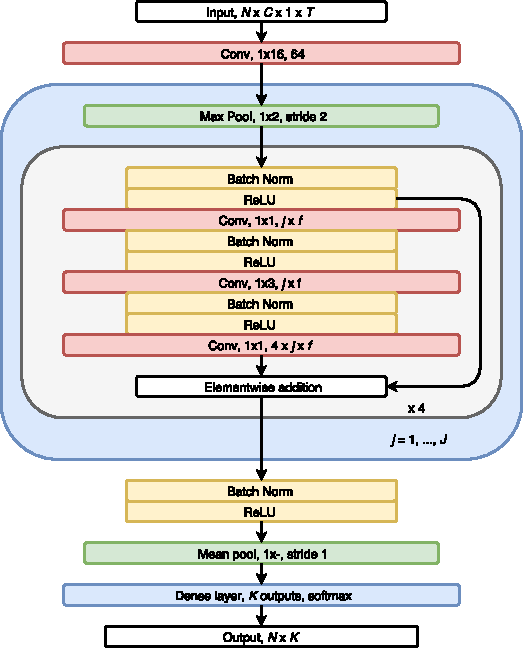
\includegraphics[height=0.5\textheight]{figures/ResNet_EMBC_compressed.pdf}
    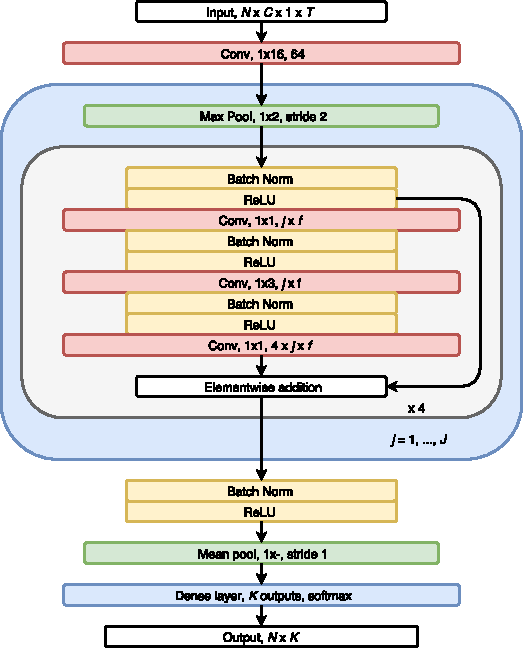
\includegraphics[width=0.9\textwidth]{figures/ResNet_EMBC_compressed.pdf}
    \caption[\acs{MASSC} network architecture]{\ac{MASSC} network architecture. The input tensor containing \ac{EEG}, \ac{EOG}, and \ac{EMG} has shape $(N, C, 1, T)$, where $N$, $C=5$, $T=6000$ correspond to the batch size, number of signals, and length of each \SI{30}{\second} epoch, respectively. The output tensor has shape $N\times K$ with $K=5$ sleep stages, while $L=4$, and $f=16$ is the number of block layers and base number of filters.}
    \label{fig:sleep-stages:network}
    \end{adjustwidth*}
\end{figure}
The residual network model is illustrated in~\cref{fig:sleep-stages:network}. 
Briefly, the bulk network comprised 50 convolutional (conv) and dense layers arranged in four block layers of four bottlenecked residual blocks each. 

A single bottleneck residual block contains three triplets of a batch normalization layer, a \ac{ReLU} activation layer, and a conv layer. 
This pre-activation configuration has shown benefits with regards to trainability and generalization compared to vanilla residual blocks~\cite{He2016b}.
Projection shortcuts were used between the first \ac{ReLU} and conv layers to the output of the last conv layer.
Kernel sizes were set to $1\times1$ for the first and third conv layers, and $1\times3$ for the second conv layer.
The number of output filters for each residual block was $l\times f$ with $l$ being the block layer index and $f=16$, resulting in a total of 256 filters after the final conv layer.

Prior to the bottleneck blocks, the input tensor $\mathbf{X}$ was passed through an initial conv layer consisting of 64 $1\times16$ filters, and then through a maximum pooling (max pool) layer with a $1\times2$ kernel and stride size, effectively reducing the time-resolution by a factor of 2.
This max pool operation was implemented in the beginning of each block layer.

The output tensor from the block layers was subsequently passed to a final batch normalization and \ac{ReLU} activation layer, followed by a mean pooling layer to reduce the tensor to $\mathbf{X} = \left(x_{nk}\right) \in \real{N\times 256}$.
Finally, a fully connected layer with $K=5$ output units corresponding to the sleep stages resulted in the following output tensor
\begin{equation}
    \mathbf{P} = \left(p_{nk}\right) \in \real{N \times K}, \quad p_{nk} = \frac{\exp{(z_{nk})}}{\sum_{k}^{K} \exp{(z_{nk})}}
\end{equation}
with $p_{nk}$ containing the softmax activations of the output units $z_{nk}$ from the fully connected layer for the $n$th subject and the $k$th sleep stage.
The predicted class for the $n$th subject can then be calculated as
\begin{equation}\label{eq:argmax}
    \hat{y}_n = \argmax_{k} p_{nk}.
\end{equation}

\paragraph{Training setup}
The optimization problem was constructed using cross entropy loss across $K$ classes and $N$ epochs as objective function, such that
\begin{equation}
    \mathcal{L}(\mathbf{p}_{n} |\, \mathbf{y}_{n},\boldsymbol{\theta}_w) = -\sum_{k=1}^{K}{y_{nk}\log{p_{nk}}},
\end{equation}
is the calculated cross entropy loss for epoch $n$ given predicted class probabilities $\mathbf{p}_n$, true class labels $\mathbf{y}_n$, and the set of current weights $\boldsymbol{\theta}_w$.
Then, the average cost across a batch of data is
\begin{equation}
    \mathcal{C}(\mathbf{P} |\, \mathbf{Y},\boldsymbol{\theta}_w) = \frac{1}{N}\sum_{n=1}^{N}{\mathcal{L}(\mathbf{p}_{n} | \mathbf{y}_{n},\boldsymbol{\theta}_w)}\label{eq:cost}.
\end{equation}
The cost function was optimized using the Adam optimization algorithm with default hyperparameters~\cite{Kingma2015}.
Weights were initialized using variance scaling~\cite{He2015a}, and we applied weight decay during training with a decay factor of $\lambda=10^{-4}$.
The initial learning rate was set to $\alpha=10^{-3}$ and was multiplied by $0.1$ every \num{50000} steps.

In order to investigate the effect of the imbalanced data on the network performance, we trained the following three different configurations.
First, we defined a \textit{baseline} configuration as described in the previous sections.
The second was a \textit{weighted} configuration, where the cost function in~\cref{eq:cost} was replaced with an average weighted by the inverse frequency for the correct class, such that
\begin{equation}
    \mathcal{C}(\hat{\mathbf{Y}} |\, \mathbf{Y},\boldsymbol{\theta}_w) = \frac{\sum_{n}^{N} \omega_{n}(\mathbf{y}_{n}) \mathcal{L}(\hat{\mathbf{y}}_{n} | \mathbf{y}_{n},\boldsymbol{\theta}_w)}{\sum_{n}^{N} \omega_{n}(\mathbf{y}_{n})},
\end{equation}
where $\omega_{n}(\mathbf{y}_{n})$ is the inverse frequency for the correct class for the $n$th subject in the current batch.
Finally, a \textit{balanced} configuration was tested, in which we performed resampling of the training dataset in order to balance classes.
We oversampled the \ac{N1}, \ac{N3}, and \ac{REM} classes with replacement, while undersampling the \ac{N2} class in order to have approximately equal fractions of each class in total.

% Models were implemented in TensorFlow 1.4~\cite{Abadi2016}, and trained on a single workstation running Ubuntu 16.04 with a Ryzen 7 1700X 8-core CPU, an NVIDIA GTX 1080 Ti GPU with 11 GB memory, and 32 GB RAM memory.

\subsubsection{Performance metrics}
Individual precision, recall and F1 scores (Pr, Re, F1) were calculated for each sleep stage and subsequently aggregated for each recording by stage frequency weighting, such that
\begin{equation}
    \mathrm{Pr}_{nk} = \frac{\mathrm{TP}}{\mathrm{TP} + \mathrm{FP}}, \quad \mathrm{Pr}_{n} = \frac{\sum_{k}{\beta_{nk} \mathrm{Pr}_{nk}}}{\sum_{k}\beta_{nk}}
\end{equation}
\begin{equation}
    \mathrm{Re}_{nk} = \frac{\mathrm{TP}}{\mathrm{TP} + \mathrm{FN}}, \quad \mathrm{Re}_{n} = \frac{\sum_{k}{\beta_{nk} \mathrm{Re}_{nk}}}{\sum_{k}\beta_{nk}}
\end{equation}
\begin{equation}
    \mathrm{F1}_{nk} = 2 \cdot \frac{\mathrm{Pr}_{nk} \cdot \mathrm{Re}_{nk}}{\mathrm{Pr}_{nk} + \mathrm{Re}_{nk}}, \quad \mathrm{F1}_{n} = \frac{\sum_{k}{\beta_{nk} \mathrm{F1}_{nk}}}{\sum_{k}\beta_{nk}},
\end{equation}
where $\beta_{nk}$ is the frequency of stage $k$ for recording $n$, and TP, FP and FN are true positives, false positive, and false negatives, respectively. 
Overall accuracy (Acc) and Cohen's kappa ($\kappa$) were also calculated for each recording.
All metrics were summarized by mean and standard deviations.

\subsubsection{Statistical tests}
Demographic and \ac{PSG} variables were tested with \acp{ANOVA} after establishing normality, while gender was tested with a $\chi^{2}$ test.
Significance was set at $\alpha=0.05$.

\subsection{Results and discussion}
Performance metrics for the train and eval subgroups are shown in~\cref{tab:sleep-stages:train_eval_performance}.
Not accounting for Pr, the baseline configuration compares favorably to the weighted and balanced configurations on both subgroups with an average accuracy of \SI{85.0}{\percent} and a Cohen's kappa of \SI{75.4} on the eval subgroup.
Since the training data is imbalanced in favor of \ac{N2}, it would be fair to assume overfitting to the majority class.
However, the lower spread in both precision and recall does not support this.

\begin{figure}[tb]
\begin{adjustwidth*}{}{-\marginparwidth-\marginparsep}
    \centering
    % 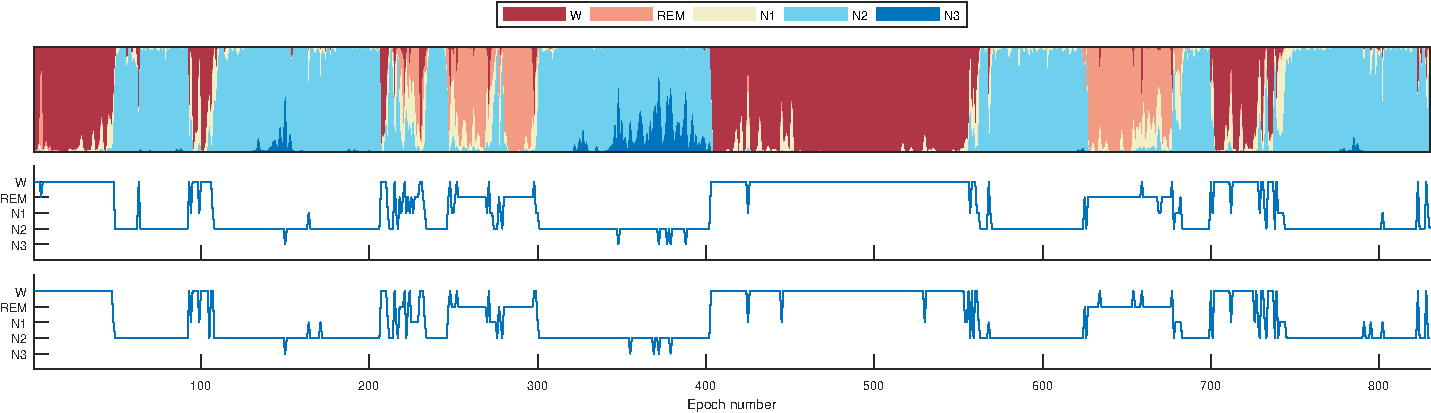
\includegraphics[width=\linewidth]{figures/test_maxacc_id1627-eps-converted-to.pdf}
    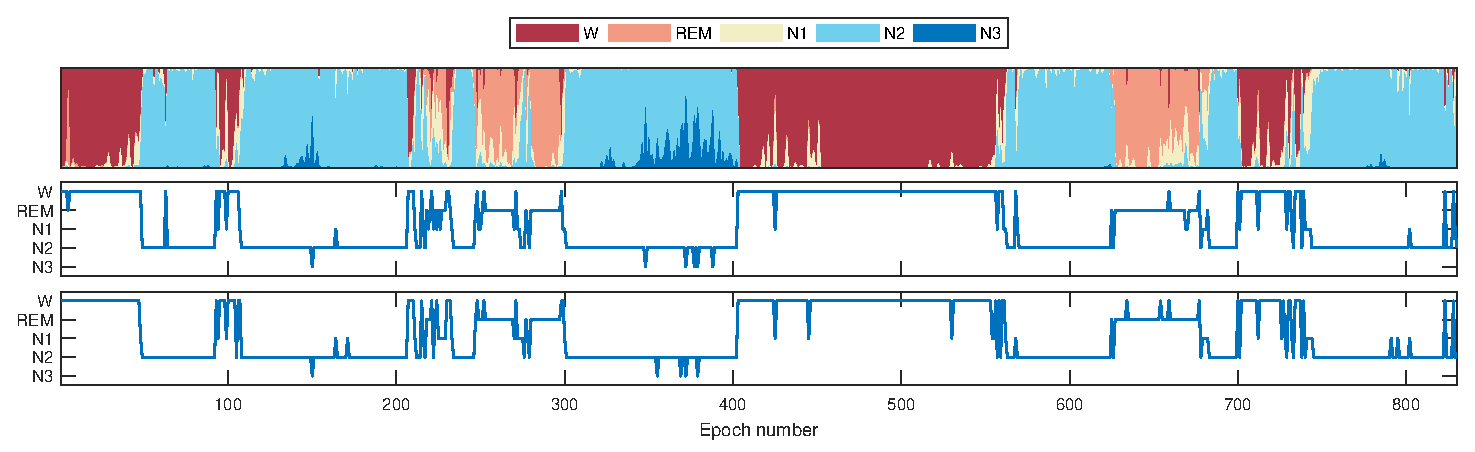
\includegraphics[width=\linewidth]{figures/paper-i/test_maxacc_id1627.eps}
    \caption[\acs{MASSC} hypnodensity example]{Top: hypnodensity graph of per-epoch probability distributions, middle: automatically scored hypnogram by applying~\cref{eq:argmax}. Bottom: manually scored hypnogram. Note the intrusions of \ac{N3} into \ac{N2} around epoch 150 and 370, and \ac{N1} into \ac{W} around 420.}
    \label{fig:slee-stages:hypnodensity}
\end{adjustwidth*}
\end{figure}

\begin{table}
    \small
    % increase table row spacing, adjust to taste
    % \renewcommand{\arraystretch}{1.3}
    \centering
    \begin{threeparttable}
    \caption[\acs{MASSC} train and validation performance, \acs{WSC}]{Averaged performance metrics for configurations.}% across train and eval subgroups.}
    \label{tab:sleep-stages:train_eval_performance}
    \begin{tabular}{@{}clccc@{}}
        \toprule
                              &          & \textbf{Baseline}          & \textbf{Weighted}          & \textbf{Balanced}          \\ \midrule
        \multirow{5}{*}{\textbf{Train}} & Acc, \%      & $ \mathbf{86.1 \pm 5.5} $ & $ 79.4 \pm 7.1 $ & $ 80.4 \pm 7.3 $ \\
                              & $\kappa$, \% & $ \mathbf{77.1 \pm 8.6} $ & $ 69.5 \pm 9.7 $ & $ 70.7 \pm 9.8 $ \\
                              & Pr, \%       & $ 87.1 \pm 4.9 $ & $ 88.7 \pm 4.1 $ & $ \mathbf{88.9 \pm 4.0} $ \\
                              & Re, \%       & $ \mathbf{86.1 \pm 5.5} $ & $ 79.4 \pm 7.1 $ & $ 80.4 \pm 7.3 $ \\
                              & F1, \%       & $ \mathbf{85.3 \pm 6.1} $ & $ 81.8 \pm 6.6 $ & $ 82.6 \pm 6.9 $ \\ \midrule
        \multirow{5}{*}{\textbf{Eval}}  & Acc, \%      & $ \mathbf{85.0 \pm 6.1} $ & $ 78.4 \pm 7.3 $ & $ 79.7 \pm 7.4 $ \\
                              & $\kappa$, \% & $ \mathbf{75.4 \pm 9.5} $ & $ 68.1 \pm 10.5 $ & $ 69.7 \pm 10.0 $ \\
                              & Pr, \%       & $ 86.3 \pm 5.3 $ & $ 87.8 \pm 4.8 $ & $ \mathbf{88.0 \pm 4.9} $ \\
                              & Re, \%       & $ \mathbf{85.0 \pm 6.1} $ & $ 78.4 \pm 7.3 $ & $ 79.7 \pm 7.4 $ \\
                              & F1, \%       & $ \mathbf{84.0 \pm 7.2} $ & $ 80.7 \pm 7.1 $ & $ 81.9 \pm 7.1 $ \\ \bottomrule
    \end{tabular}
    \begin{tablenotes}
    \item Metrics are shown as mean \(\pm\) standard deviations across each \ac{PSG}. Best performing model for each metric is shown in bold.
    \end{tablenotes}
    \end{threeparttable}
\end{table}

\begin{table}[tb]
    \small
    % increase table row spacing, adjust to taste
    % \renewcommand{\arraystretch}{1.3}
    \setlength{\tabcolsep}{4pt}
    \caption[\acs{MASSC} test group confusion matrix, \acs{WSC}]{Aggregated confusion matrix and stage-specific performance metrics in test subgroup.}
    \label{tab:sleep-stages:test_performance_aggregated}
    \centering
    \begin{threeparttable}
    \begin{tabular}{@{}llcccccccc@{}}
        \toprule
         & & \multicolumn{5}{c}{\textbf{Automatic}} & & & \\ \cline{2-7}
                 & \acs{W}     & \acs{W}   & \acs{N2}    & \acs{N3}   & \acs{REM}   & Pr, \% & Re, \% & F1, \% \\ \midrule
        \multirow{5}{*}{\textbf{Manual}} & \acs{W}        & 37980 & 1322 & 852   & 2    & 327   & 84.3    & 93.8    & 88.8    \\
         & \acs{W}       & 3922  & 8784 & 3545  & 0    & 2193  & 51.9    & 47.6    & 49.7    \\
         & \acs{N2}       & 1756  & 5136 & 99564 & 1091 & 991   & 88.6    & 91.7    & 90.2    \\
         & \acs{N3}       & 18    & 1    & 7932  & 4063 & 14    & 78.8    & 33.8    & 47.3    \\
         & \acs{REM}        & 1361  & 1680 & 465   & 0    & 23931 & 87.2    & 87.2    & 87.2    \\ \bottomrule
    \end{tabular}
    \begin{tablenotes}
        \small
        \item%
        \describe{W}; %
        \describe{N1}; %
        \describe{N2}; %
        \describe{N3}; %
        \describe{REM}.
    \end{tablenotes}
    \end{threeparttable}
\end{table}


Evaluating the baseline model on the test subgroup, only a slight drop in accuracy and $\kappa$ is observed, indicating that the model generalizes well, see~\cref{tab:sleep-stages:test_performance_aggregated} and~\cref{tab:sleep-stages:test_performance_average}.
The lowest sensitivity is obtained for \ac{N1} and \ac{N3}, which is in accordance with clinical experience reported in the literature~\cite{Younes2017, Rosenberg2013, Norman2000, Younes2016}.
N1 is a transitional stage between wakefulness, drowsiness and sleep often containing beta and alpha activity in epochs of low interscorer agreement, which explains the low predictive power in the confusion matrix.
The sleep continuum is also apparent in~\cref{fig:slee-stages:hypnodensity} which shows the manually and automatically scored hypnograms in the middle and bottom traces, and the hypnodensity graph in the top trace for a representative subject in the test subgroup.
The hypnodensity is a probabilistic representation of the hypnogram, which has found use in the detection of narcolepsy and Parkinson's disease~\cite{Koch2014, Christensen2014, Stephansen2018}.

Our baseline model attains favorable performance when comparing to the results reported for the raw waveform CNN model in~\cite{Biswal2017} with both higher accuracy and Cohen's kappa.
However, it should be stressed that~\cite{Biswal2017} only used \ac{EEG} channels from 9000 recordings, while our model uses both \ac{EEG}, \ac{EOG} and \ac{EMG} data, but only from 1850 recordings.
Furthermore, our baseline model performs only slightly worse compared to the best-performing model in~\cite{Biswal2017} without using any memory networks.
This indicates a performance gain by adding recurrent networks, such as long short-term memory cells, to our network.

A possible limiting factor to our model is the filter kernels.
The small filter sizes in block layers might not be able to accurately capture the physiological dynamics, but there are indications that many, smaller kernels are preferable to fewer, larger kernels when comparing model complexity versus computational costs~\cite{Szegedy2015}.

Future work will include adding more data to balance classes, and adding long short-term memory cells to the network in order to model temporal dynamics between epochs.
\begin{table}[tb]
    \small
    \centering
    \begin{threeparttable}
    \caption[MASSCv1 overall test performance, \acs{WSC}]{Performance across recordings in test subgroup.}
    \label{tab:sleep-stages:test_performance_average}
    \begin{tabular}{@{}ccccc@{}}
    \toprule
        \textbf{Accuracy}              & $\boldsymbol{\kappa}$         & \textbf{Pr}               & \textbf{Re}               & \textbf{F1}               \\ \midrule
        $ 84.1 \pm 6.9 $ & $ 0.746 \pm 0.099 $ & $ 85.7 \pm 6.1 $ & $ 84.1 \pm 6.9 $ & $ 83.1 \pm 7.6 $ \\ \bottomrule
    \end{tabular}
    \begin{tablenotes}
    \item Values are shown as mean \(\pm\) standard deviation across \acs{PSG}. Pr: precision; Re: recall.
    \end{tablenotes}
    \end{threeparttable}
\end{table}

\clearpage\section{Paper II: Automatic sleep stage classification with deep residual networks in a mixed-cohort setting}\label{sec:paperii}
\sectionmark{Olesen, Jennum, Mignot, \& Sorensen, 2020b (\textit{under review)}}

\begin{tcolorbox}[colframe=white]
\paragraph{Study Objectives:} Sleep stage scoring is performed manually by sleep experts and is prone to subjective interpretation of scoring rules with low intra- and interscorer reliability. 
Many automatic systems rely on few small-scale databases for developing models, and generalizability to new datasets is thus unknown. 
We investigated a novel deep neural network to assess the generalizability of several large-scale cohorts.
\paragraph{Methods:} A deep neural network model was developed using \num{15684} polysomnography studies from five different cohorts. 
We applied four different scenarios: 1) impact of varying time-scales in the model; 2) performance of a single cohort on other cohorts of smaller, greater or equal size relative to the performance of other cohorts on a single cohort; 3) varying the fraction of mixed-cohort training data compared to using single-origin data; and 4) comparing models trained on combinations of data from 2, 3, and 4 cohorts.
\paragraph{Results:} Overall classification accuracy improved with increasing fractions of training data (0.25\%: \ci{0.782}{0.097}{0.777}{0.787}; 100\%: \ci{0.869}{0.064}{0.864}{0.872}), and with increasing number of data sources (2: \ci{0.788}{0.102}{0.787}{0.790}; 3: \ci{0.808}{0.092}{0.807}{0.810}; 4: \ci{0.821}{0.085}{0.819}{0.823}). 
Different cohorts show varying levels of generalization to other cohorts.
\paragraph{Conclusions:} Automatic sleep stage scoring systems based on deep learning algorithms should consider as much data as possible from as many sources available to ensure proper generalization. 
Public datasets for benchmarking should be made available for future research.
\end{tcolorbox}


\subsection{Cohort descriptions}
To investigate and conclude on generalizability of any machine learning or sleep stage classification model, multiple heterogenous datasets must be used for training, validation and testing purposes.
In this work, we collected datasets from five different sources, each dataset containing a diverse collection of subjects presenting with multiple disease phenotypes.
Details of the separate cohorts are shown in~\cref{tab:sleep-stages:paperii:table-01} along with reported \textit{p}-values highlighting cohort differences.
Each cohort was split into a training, validation and testing subset in proportions of \SI{87.5}{\percent}, \SI{2.5}{\percent}, and \SI{10}{\percent}, respectively, using random sampling without replacement among unique subjects, so that no subject is shared between subsets.
With these percentages, we maximize the number of \acp{PSG} available for training, while still reserving enough \acp{PSG} for validation and testing.
Collecting all the separate subsets across cohorts forms a training, validation, and testing partition, containing the respective subsets from all five cohorts. 

\subsubsection{\ac{ISRUC}}
This cohort contains 126 recordings from 118 unique subjects recorded at the Sleep Medicine Centre of the Hospital of Coimbra University, Portugal, in the period 2009–2013~\cite{Khalighi2016}.
The cohort comprises three subgroups: subgroup I contains 100 \acp{PSG} of subjects with diagnosed sleep disorders, generally sleep apnea; subgroup II contains 16 recordings of eight subjects most of which are also diagnosed with sleep apnea; and subgroup III contains recordings from 10 subjects with no diagnosed sleep disorders.
All \acp{PSG} were recorded with the same recording hardware and software and each was scored by two technicians for sleep stages and sleep events according to the \ac{AASM} guidelines.
\ac{ISRUC} is a freely accessible resource and all data and \ac{PSG} files can be located at \url{https://sleeptight.isr.uc.pt/ISRUC_Sleep/}.

\subsubsection{\ac{MrOS}}
The \ac{MrOS} Sleep Study is part of the larger Osteoporotic Fractures in Men Study, which aims to understand the relationships between sleep disorders, fractures, and vascular diseases in community-dwelling men~\cite{Blank2005, Orwoll2005, Blackwell2011}. 
It consists of 2907 in-home \ac{PSG} recordings with an additional 1026 follow-up \ac{PSG} studies from subjects recruited from six different clinical centers in the USA.
Each recording was annotated by an expert technician according to Rechtschaffen and Kales (R\&K) criteria for sleep staging~\cite{Rechtschaffen1968}.
For compatibility with \ac{AASM} guidelines, we combined stages labeled S3 and S4 into \ac{N3}. All data were accessed from the \ac{NSRR} repository~\cite{Dean2016, Zhang2018}.

\subsubsection{\ac{SHHS}}
The \ac{SHHS} is a large, multi-center study on cardiovascular outcomes related to sleep disorders with a specific focus on sleep-disordered breathing~\cite{Quan1997, Redline1998}.
The cohort consists of 6441 subjects above 40 years old recruited between 1995 and 1998 undergoing in-home \ac{PSG} (\ac{SHHS} Visit 1) with subsequent follow-up \ac{PSG} between 2001 and 2003 in 3295 subjects (\ac{SHHS} Visit 2).
\ac{PSG} recordings were annotated for sleep stages by trained and certified technicians according to R\&K rules.
From the original cohort we extracted 5793 \acp{PSG} and annotations from Visit 1, and 2651 from Visit 2.
We aggregated S3 and S4 stages into \ac{N3} similar to \ac{MrOS}.
All data were accessed from \ac{NSRR} repository.

\subsubsection{\ac{WSC}}
\ac{WSC} is a population-based study of sleep-disordered breathing in government workers in Wisconsin, USA, that was initiated in 1988~\cite{Young1993, Young2008}.
In this work, we used 2412 \acp{PSG} from 1091 unique subjects in the \ac{WSC} sample scored by expert technicians according to R\&K rules with subsequent merging of S3 and S4 into \ac{N3}.

\subsubsection{\ac{SSC}}
\acp{PSG} from this cohort originate from patients referred for sleep disorders evaluation and recorded at the Stanford Sleep Clinic since 1999.
The specific sample used in this study represents a small subset ($n=772$) of the whole cohort, which was selected and described in detail in previous studies scored according to R\&K or \ac{AASM} guidelines according to prevailing standard at the time of evaluation~\cite{Andlauer2013, Moore2014}. 

\begin{landscape}
% \begin{sidewaystable}
\begin{table}[tb]
\begin{adjustwidth*}{}{-\marginparwidth-\marginparsep}
\centering
\small
\begin{threeparttable}
\caption{Cohort demographics}
\label{tab:sleep-stages:paperii:table-01}
\begin{tabular}{@{}lllllll@{}}
\toprule
           & \textbf{\ac{ISRUC}}                             & \textbf{\ac{MrOS}}                              & \textbf{\ac{SHHS}}                              & \textbf{\ac{SSC}}                               &\textbf{\ac{WSC}}                               & \textbf{\textit{p}-value}   \\ \midrule
N (female) & 126 (50)                          & 3932 (0)                          & 8444 (4458)                       & 767 (319)                         & 2401 (1103)                       & ---         \\
Age, years & 49.8$\pm$15.9 {[}20.0--85.0{]}   & 77.6$\pm$5.6 {[}67.0--90.0{]}    & 64.5$\pm$11.2 {[}39.0--90.0{]}   & 45.7$\pm$14.5 {[}13.0--104.8{]}  & 59.7$\pm$8.4 {[}37.2--82.3{]}    & \num{<0.0001}         \\
BMI, kg/m2 & ---       & 27.1$\pm$3.8 {[}16.0--47.0{]}    & 28.2$\pm$5.1 {[}18.0--50.0{]}    & 27.2$\pm$6.5 {[}9.8--78.7{]}     & 31.6$\pm$7.2 {[}17.5--70.6{]}    & \num{<0.0001} \\
TST, min   & 350.0$\pm$67.3 {[}87.5--479.0{]} & 352.1$\pm$71.9 {[}39.0--626.0{]} & 374.1$\pm$69.4 {[}68.0--605.0{]} & 361.0$\pm$83.5 {[}0.0--661.0{]}  & 364.1$\pm$63.6 {[}19.5--575.0{]} & \num{<0.0001}  \\
SL, min    & 17.7$\pm$20.5 {[}0.0--144.5{]}   & 24.7$\pm$26.9 {[}1.0--402.0{]}   & 24.2$\pm$25.7 {[}0.0--349.0{]}   & 93.5$\pm$58.9 {[}0.5--404.0{]}   & 33.2$\pm$21.4 {[}0.5--333.0{]}   & \num{<0.0001}         \\
REML, min  & 125.6$\pm$61.4 {[}7.0--323.0{]}  & 104.8$\pm$75.1 {[}0.0--590.0{]}  & 91.7$\pm$58.8 {[}0.0--471.0{]}   & 140.9$\pm$88.0 {[}0.0--464.0{]}  & 128.3$\pm$76.0 {[}3.5--514.0{]}  & \num{<0.0001} \\
WASO, min  & 76.2$\pm$49.8 {[}7.5--251.0{]}   & 117.5$\pm$67.6 {[}4.0--487.0{]}  & 80.2$\pm$54.7 {[}2.0--378.0{]}   & 79.5$\pm$55.0 {[}3.5--367.0{]}   & 73.6$\pm$45.9 {[}3.0--325.0{]}   & \num{<0.0001} \\
SE, \%     & 78.8$\pm$14.1 {[}19.5--98.3{]}   & 75.5$\pm$12.4 {[}12.0--99.0{]}   & 80.5$\pm$11.0 {[}11.3--99.0{]}   & 77.4$\pm$14.8 {[}0.0--98.0{]}    & 77.1$\pm$11.2 {[}4.1--95.6{]}    & \num{<0.0001} \\
N1, \%     & 13.3$\pm$5.8 {[}1.8--33.1{]}     & 8.3$\pm$6.4 {[}0.0--70.0{]}      & 5.5$\pm$4.0 {[}0.0--39.1{]}      & 11.7$\pm$10.2 {[}0.0--92.0{]}    & 10.8$\pm$6.9 {[}1.0--88.4{]}     & \num{<0.0001}         \\
N2, \%     & 31.9$\pm$10.3 {[}4.4--89.3{]}    & 62.5$\pm$10.0 {[}21.0--95.0{]}   & 56.9$\pm$11.5 {[}10.9--100.0{]}  & 62.8$\pm$24.9 {[}0.0--636.0{]}   & 66.0$\pm$9.4 {[}9.1--93.3{]}     & \num{<0.0001}         \\
N3, \%     & 19.6$\pm$8.0 {[}0.0--41.1{]}     & 36.0$\pm$31.8 {[}0.0--259.0{]}   & 17.5$\pm$11.6 {[}0.0--70.1{]}    & 9.0$\pm$9.3 {[}0.0--73.0{]}      & 7.2$\pm$7.8 {[}0.0--47.5{]}      & \num{<0.0001}         \\
REM, \%    & 13.3$\pm$6.3 {[}0.0--37.8{]}     & 19.3$\pm$6.8 {[}0.0--44.0{]}     & 20.1$\pm$6.3 {[}0.0--48.0{]}     & 16.3$\pm$7.2 {[}0.0--40.0{]}     & 16.0$\pm$6.2 {[}0.0--38.2{]}     & \num{<0.0001} \\
ArI, /h    & 20.2$\pm$10.0 {[}2.1--72.0{]}    & 23.7$\pm$12.1 {[}1.0--105.0{]}   & 18.9$\pm$10.5 {[}0.0--110.4{]}   & 125.0$\pm$124.2 {[}1.0--729.0{]} & ---       & \num{<0.0001}         \\
AHI, /h    & 13.1$\pm$13.2 {[}0.0--82.2{]}    & 13.7$\pm$14.6 {[}0.0--89.0{]}    & 18.1$\pm$16.2 {[}0.0--161.8{]}   & 13.5$\pm$19.2 {[}0.0--98.6{]}    & 7.0$\pm$9.4 {[}0.0--72.6{]}      & \num{<0.0001}         \\
PLMI, /h   & 8.0$\pm$27.4 {[}0.0--292.8{]}    & 35.7$\pm$37.5 {[}0.0--233.0{]}   & ---       & 7.0$\pm$18.1 {[}0.0--139.9{]}    & ---       & \num{<0.0001} \\ \bottomrule
\end{tabular}
\begin{tablenotes}
\item %
\describe{BMI}; %
\describe{TST}; %
SL: sleep latency; %
\describe{REML}; %
\describe{WASO}; %
SE: sleep efficiency; %
\describe{N1}; %
\describe{N2}; %
\describe{N3}; %
\describe{REM}; %
\describe{ArI}; %
\describe{AHI}; %
\describe{PLMI}; %
\describe{ISRUC}; %
\describe{MrOS}; %
\describe{SHHS}; %
\describe{SSC}; %
\describe{WSC}; %
\end{tablenotes}
\end{threeparttable}
\end{adjustwidth*}
\end{table}
% \end{sidewaystable}
\end{landscape}

\begin{figure}[tb]
\begin{adjustwidth*}{}{-\marginparwidth-\marginparsep}
    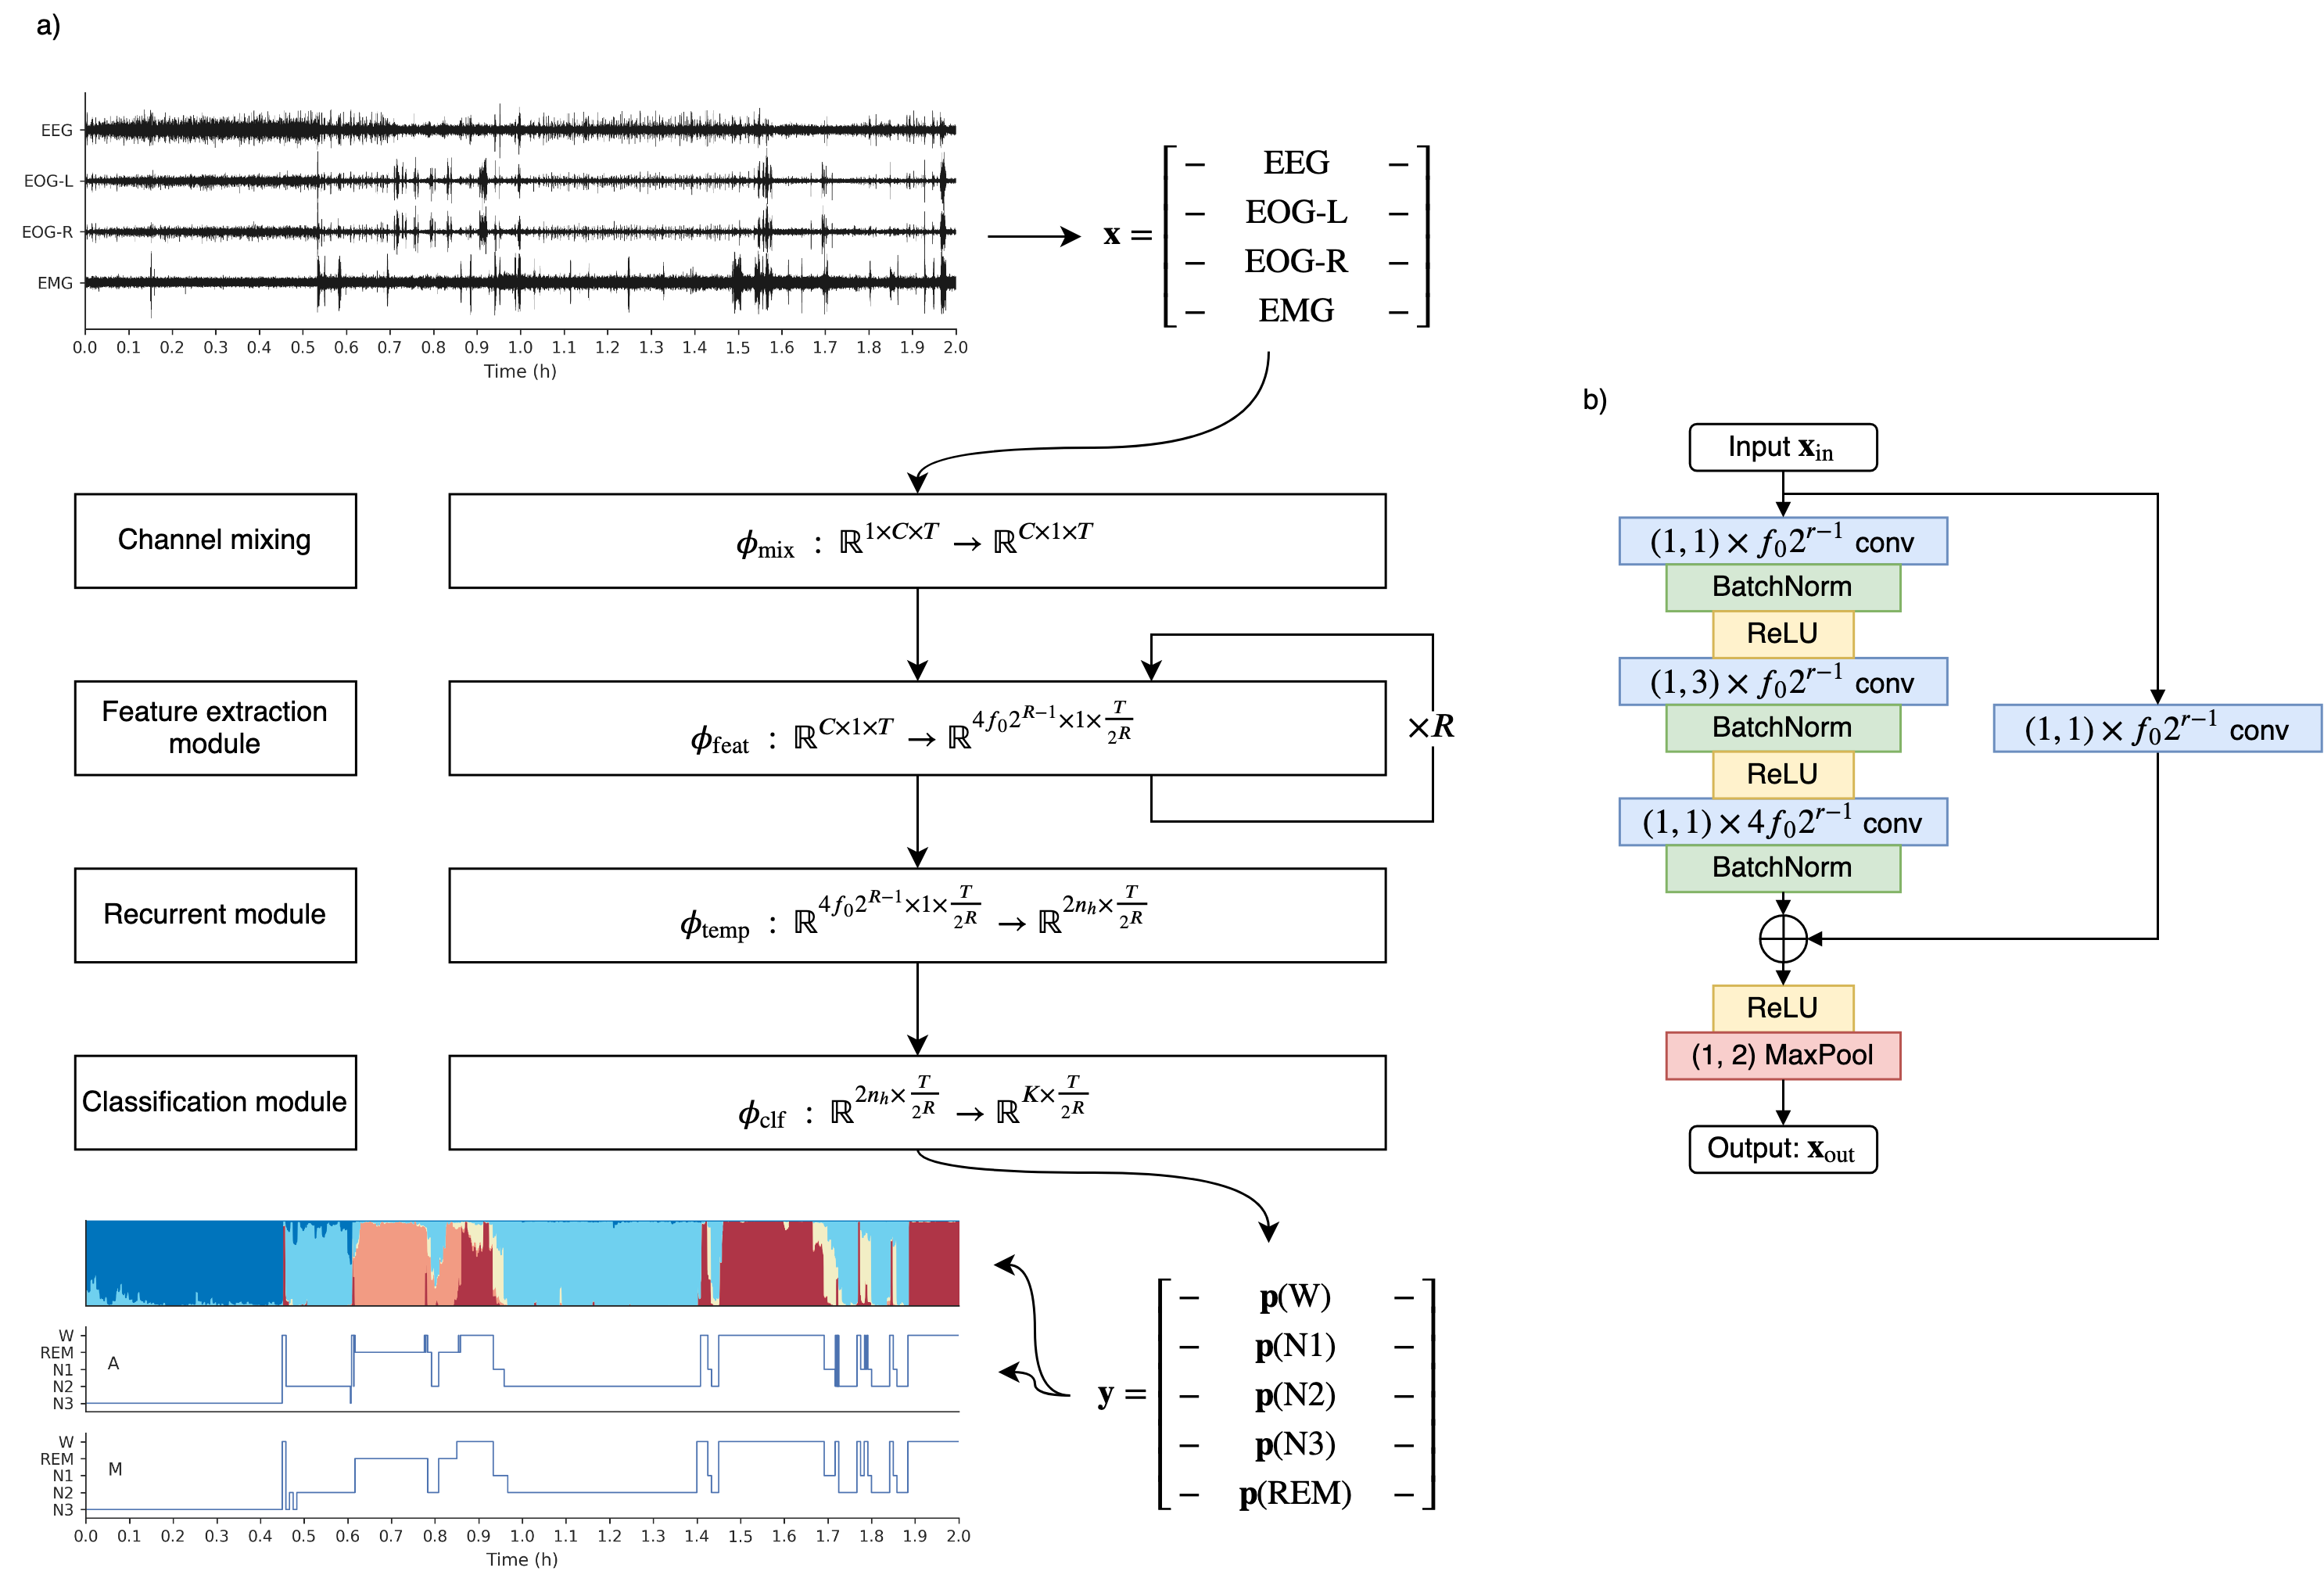
\includegraphics[width=\linewidth]{figures/paper-ii/figure_network.png}
    \caption[\acs{MASSC}v2 model overview]{Model overview. a) The input is a sequence of data \(\mathbf{x}\) containing raw signal data from \ac{EEG}, left/right \ac{EOG}, and \ac{EMG} channels, which is supplied to the network modules in sequence. The feature extraction module consists of \(R\) repeated blocks of residual units, see b) panel to the right. The output of the model is a matrix \(\mathbf{y}\) containing class probabilities for each sleep stage for each time step, which can be visualized either directly as a hypnodensity, or by \(\argmax{\mathbf{y}}\) as a hypnogram. The \textbf{A} and \textbf{M} labels in the hypnogram plots corresponds to automatic and manually scored hypnograms. b) Schematic of a single residual block in the feature extraction module. Convolutional layers are described by the kernel size \(\times\) number of filters using a stride value of 1. Shortcut uses \(1\times1\) convolutions with added zero-padding to maintain temporal dimension. Conv, convolutional layer; BatchNorm, batch normalization; \describe{ReLU}; \(f_0\), base number of filters (\(f_0=4\)).}
    \label{fig:sleep-stages:paper-ii:figure-01}
\end{adjustwidth*}
\end{figure}

\subsection{Methods}

\subsubsection{Data pipeline}
Electrophysiological signals corresponding to the minimum acceptable montage for sleep staging available across all cohorts were extracted for each \ac{PSG}.
These included a central \ac{EEG} (either C3 or C4 referenced to the contra-lateral mastoid), left and right \ac{EOG} referenced to the contra-lateral mastoid, and a single submentalis \ac{EMG}.
The choice between C3 and C4 was determined based on the lowest total signal energy across the entire duration of the \ac{PSG} to avoid excessive signal popping.
Other methods to determine appropriate channels include algorithms based on shortest Mahalanobis distance to an already determined reference distribution~\cite{Stephansen2018}, but was not investigated in this study.
All signals were resampled to $f_s = \SI{128}{\hertz}$ using a polyphase filtering procedure irrespective of original sampling frequency, and subsequently filtered using a zero-phase approach with \nth{4} order Butterworth IIR filters (\SIrange{0.5}{35}{\hertz} band-pass for \ac{EEG} and \ac{EOG}; \SI{10}{\hertz} high-pass for \ac{EMG}) in accordance with \ac{AASM}2020 filter specifications~\cite{Berry2020}.
Each signal was normalized to zero mean and unit variance to accommodate differences in recording equipment and baselines, and to compress the dynamic range into something easily trainable for the neural network architecture.
We denote by $C$ the number of input signals supplied to the neural network, where in this case $C=4$.

\subsubsection{Machine learning problem}
We designate by $\mathcal{X} \in \real{C \times T}$ the set of \SI{30}{\second} input data segments with $S$ input channels and segment length $T$, and the corresponding sleep stage classifications by $\mathcal{Y} = \lbrace y \in \real{K}_{+} \mid \sum_i y_i = 1 \rbrace$, where $K = 5$ corresponds to the five sleep stages.
Thus, $y$ is a probability simplex, which maps to the ordered set $\mathcal{S} = \lbrace \wake, \nI, \nII, \nIII, \rem \rbrace$ by the argmax function such that $\argmax{y : \mathcal{Y} \to \mathcal{S}}$.
Furthermore, as we are potentially interested in classifying multiple sleep stages at once, we extend the problem of classifying a single sleep stage given $x \in \mathcal{X}$ to a sequence-to-sequence problem, in which we desire to learn a differentiable function representation $\Phi$, that maps a sequence of \SI{30}{\second} epochs $\mathbf{x} \in \real{C \times \alpha T}$ to their corresponding label probabilities $\mathbf{y} \in \real{K \times \alpha}$, where $\alpha$ is a parameter that controls the sequence length. 
For example, if $\alpha=8$, the sequence $\mathbf{x}$ contains \SI{4}{\minute} of successive \ac{PSG} data described by 8 epochs of length \SI{30}{\second}.
Furthermore, we denote by $\llbracket a, b \rrbracket$ the set of integers from $a$ to $b$, i.e. $\llbracket a, b \rrbracket = \lbrace n \in \mathbb{N} \mid a \leq n \leq b \rbrace$, and by $\llbracket N \rrbracket$ the shorthand form of $\llbracket 1, N \rrbracket$.

\subsubsection{Network architecture}

\begin{table}[t]
% \centering
\begin{adjustwidth*}{}{-\marginparwidth-\marginparsep}
\raggedleft
\begin{threeparttable}
    \small
    % \begin{adjustwidth*}{}{-\marginparwidth-\marginparsep}
    \caption[\acs{MASSC}v2 model architecture]{Overview of model architecture.}
    \label{tab:sleep-stages:paperii:table-02}
    \begin{tabular}{@{}lllllll@{}} \toprule
    \textbf{Module} & \textbf{Type} & \textbf{Filters} & \textbf{Kernel} & \textbf{Stride} & \textbf{Activation} & \textbf{Output size} \\ \midrule
    \(\mathbf{x}\) & Input & --- & --- & --- & --- & \(1 \times C \times T\) \\ \midrule
    \(\varphi_\text{mix}\) & \twod conv. & \(C\) & \((1, C)\) & 1 & \acs{BN}+\acs{ReLU} & \(C \times 1 \times T\) \\ \midrule
    \(\varphi_\text{feat}^{(r)}\) & Res. block\(^{\dagger}\) & \(f_0 2^{r-1}\) & \((1, 1)\) & \((1, 1)\)  & \acs{BN}+\acs{ReLU} & \(f_0 2^{r-1} \times 1 \times \frac{T}{2^{r-1}}\) \\
    \(r \in \llbracket R \rrbracket\)& & \(f_0 2^{r-1}\) & \((1, 3)\) & \((1, 2)\) & \acs{BN}+\acs{ReLU}  & \(f_0 2^{r-1} \times 1 \times \frac{T}{2^r}\) \\ \midrule
    & & \(4f_0 2^{r-1}\) & \((1, 1)\) & \((1, 1)\) & \acs{BN}+\acs{ReLU} & \(f_0 2^r \times 1 \times \frac{T}{2^r}\) \\
    \(\varphi_\text{temp}\) & \acs{bGRU} & \(n_h\) & --- & --- & --- & \(2n_h \times \frac{T}{2^R}\) \\ \midrule
    \(\varphi_\text{clf}\) & \oned conv. & \(K\) & \(2n_h\) & 1 & Softmax & \(K \times \frac{T}{2^R}\) \\ \bottomrule
    \end{tabular}
    \begin{tablenotes}
        \small
        \item Kernel sizes correspond to the first, second and third convolutional layer in each residual block. Stride counts correspond to the residual block and the subsequent maxpooling operation. %
        Conv., convolution; %
        Res. block, residual block; %
        \describe{BN}, %
        \describe{ReLU}, %
        \describe{bGRU}, %
        \(C\), number of input channels; %
        \(T\), length of segment in samples; %
        \(f_0\), base number of filters in residual blocks;
        \(R\), number of residual blocks; %
        \(n_h\), number of hidden units in \acs{bGRU}; %
        \(K\), number of sleep stage classes; %
        \(^{\dagger}\)See~\cref{fig:sleep-stages:paper-ii:figure-01} for details.
    \end{tablenotes}
\end{threeparttable}
    \end{adjustwidth*}
\end{table}

As the representation of $\Phi$, we adapted and extended a previously published neural network architecture for automatic sleep stage classification, which was based on a variant of the ResNet-50 architecture commonly used for two-dimensional image classification tasks, but adapted and re-trained from scratch for the specific use-case of one-dimensional, time-dependent signals in the \ac{PSG}~\cite{Olesen2018c}.
This network has the advantage that it does not require any manual feature engineering and extraction compared to previous state of the art sleep stage classification models~\cite{Stephansen2018}.
An overview of the proposed network architecture is provided graphically in \cref{fig:sleep-stages:paper-ii:figure-01} and \cref{tab:sleep-stages:paperii:table-02}.
Briefly, the architecture consists of four modules:
\begin{enumerate}
    \item an initial mixing module 
    \begin{equation}
        \varphi_{\mathrm{mix}} : \real{1 \times C \times T} \to \real{C \times 1 \times T},
    \end{equation}%$\varphi_{\mathrm{mix}} : \real{1 \times C \times T} \to \real{C \times 1 \times T} $,
	\item a feature extraction module
	\begin{equation}
	    \varphi_{\mathrm{feat}} : \real{C \times 1 \times T} \to \real{f_0 2^{R+1} \times 1 \times T/2^R},
	\end{equation}
	\item a temporal processing module
	\begin{equation}
	    \varphi_{\mathrm{temp}}     : \real{f_0 2^{R+1} \times 1 \times T/2^R} \to \real{2n_h \times T/2^R}, \, \text{and}
	\end{equation} %$\varphi_{\mathrm{temp}}     : \real{f_0 2^{R+1} \times 1 \times T/2^R} \to \real{2n_h \times T/2^R} $, and
	\item a classification module
	\begin{equation}
	    \varphi_{\mathrm{clf}} : \real{2n_h \times T/2^R} \to \real{K \times T/2^R}.
	\end{equation}%$\varphi_{\mathrm{clf}} : \real{2n_h \times T/2^R} \to \real{K \times T/2^R}$.
\end{enumerate}
Thus, we obtain a differentiable representation of the function  $\Phi$ as
\begin{align}
\begin{split}
    &\Phi : \real{C \times K} \to \real{K \times T/2^R} \\
    &\Phi \parentheses{\mathbf{x}} = \varphi_{\mathrm{clf}} \parentheses{ \varphi_{\mathrm{temp}} \parentheses{ \varphi_{\mathrm{feat}} \parentheses{ \varphi_{\mathrm{mix}} \parentheses{ \mathbf{x} } } } }.
\end{split}
\end{align}
The output of this function is the matrix $\mathbf{y} \in \real{K \times T/2^R}$ containing sleep stage probabilities in the sequence of \ac{PSG} data evaluated every second.

\paragraph{Mixing module}
The raw input data is input to this module, which encourages non-linear channel mixing similar to what has been proposed in recent literature~\cite{Chambon2018c, Chambon2018b, Chambon2019, Olesen2019}.
The module is realized using a single \twod convolutional operation outputting $C$ feature maps computed using single-strided $(C \times 1)$ kernels followed by \ac{ReLU} activations.

\paragraph{Feature extraction (residual network) module}
This is comprised of a succession of $R$ residual blocks, which are responsible for the bulk feature extraction from the channel-mixed data, see~\cref{fig:sleep-stages:paper-ii:figure-01}.
Each residual block is realized using bottlenecks of first a $1\times 1$ convolution to reduce the number of feature maps, then a $1\times 3$ convolution, and lastly a $1 \times 1$ convolution to finally increase the number of feature maps. 
Each convolution operation is followed by a batch normalization~\cite{Ioffe2015} and ReLU activation except after the last convolutional layer, where shortcut projections are added before the activation~\cite{He2016b}.
This type of block structure enables the design and training of very deep networks without the risk of vanishing gradients due to the projection shortcuts~\cite{He2016}.

\paragraph{Temporal processing module}
This module is realized by a bidirectional \ac{GRU}~\cite{Cho2014} in order to accommodate temporal dependencies in the \ac{PSG}.
The \ac{GRU} runs through the temporal dimension of the output from $\varphi_{\mathrm{feat}}$ of $T/2^R$ time steps each containing $f_0 2^{R}$ feature maps and outputs $n_h$ new features in each direction for each time step.
By running both forward and backward, we can accommodate that technicians base their scoring on looking backwards as well as ahead in time in each time segment (typically \SI{30}{\second}).

\paragraph{Classification module}
The final module in the architecture performs actual classification based on the forward and backward features for each time step outputted from $\varphi_{\mathrm{temp}}$.
It is realized by a single convolutional operation with a subsequent softmax activation to compute a probability distribution over the $K$ sleep stage classes, such that the probability of sleep stage $i$ at time step $n$ is given by
\begin{equation}
   y_i^{(n)} = \frac{\exp{a_i}}{\sum_k{\exp{a_k}}} ,
\end{equation}
where $a_i \in \mathbf{a}$ is the activation of the last layer in the network, and $k \in \llbracket K \rrbracket$.


\subsubsection{Loss function specification}
The network was trained end-to-end with respect to a loss function, that takes the output probabilities from the network $y = \Phi(\mathbf{x})$ and calculates the loss as
\begin{align}
\begin{split}\label{eq:loss-paperII}
    \mathcal{L} \parentheses{ \mathbf{y} } &= - \sum_{n=1}^{30/\tau}\sum_{k=1}^{K} t_k^{(n)}\log{ \parentheses{ \tilde{y}^{(n)}_k }}, \\
    \tilde{y}^{(n)}_k &= \frac{1}{\tau} \sum_{\mathclap{i=\tau \parentheses{ j - 1 } + 1}}^{\tau n} y_k^{(i)},
\end{split}
\end{align}
which is the cross-entropy between successive time-averaged classifications parameterized by the number of successive one-second predictions $\tau$, and the ground truth labels $t$ broadcasted to $\sfrac{30}{\tau}$ labels per \SI{30}{\second} segment.
This way, we can acquire predictions every second, that can be combined in time at intervals given by $\tau$.

\subsubsection{Experimental setups}\label{sec:sleep-stages:paper-ii:experimental-setup}
We set up four different experiments in this study.
\begin{enumerate}
    \item We wished to investigate the effect of increasing the complexity of the recurrent module by varying the number of units $n_h$ in the module $\varphi_{\mathrm{temp}}$ in the space $n_h=2^k, k \in \llbracket 6, 11 \rrbracket$.
    We hypothesize that there exists a sweet-spot in the number of hidden units that balances computational complexity with classification performance, i.e. classifying a sequence of sleep stage labels given a corresponding sequence of outputs from $\varphi_{\mathrm{feat}}$.
    The results of this experiment were furthermore used to determine parameters for models in subsequent experiments.
    \item Since we have several cohorts at our disposition of both clinical and research origin, we can investigate the compatibility and inherent generalizability of the different cohorts in two ways: 1) we set aside a single cohort for testing, while we train the models on the remaining four (leave-one-cohort-out, \ac{LOCO} training); and 2) we train on a single cohort, while we set aside the remaining four for testing (leave-one-cohort-in, \ac{LOCI} training).
    \item Generalizability can also be investigated in another way, which can answer the question of how many data sources is necessary.
    We trained models with all possible 2-, 3-, and 4-combinations of cohorts, i.e. one run trained on \ac{ISRUC} and \ac{MrOS} training data, another run with \ac{ISRUC} and \ac{SHHS} train data, a third with \ac{ISRUC} and \ac{SSC}, etc., with all runs subjected to subsequent evaluation on the test partition. 
    \item Previous studies have already investigated the performance of automatic sleep staging algorithms using shallow machine learning models.
    At the time of writing however, none have investigated the effect of available training data for deep learning models at this magnitude (up to tens of thousands).
    We therefore trained models on \SIlist{0.25;0.5;1;5;10;25;50;75;100}{\percent} of the data available for training.
    Specifically, some of these fractions of the total number of \acp{PSG} correspond roughly to the number of \acp{PSG} in the training partitions in each cohort, allowing for direct comparisons between training a model with mixed- and single-cohort training data.
\end{enumerate}

Common for all experiments were the default parameter values $C=4$, $f_s=\SI{128}{\hertz}$, $T=\tau f_s$, $K=5$, $R=7$, and $f_0=4$ for the number of input channels, sampling frequency, the sequence length, the number of sleep stages, the number of consecutive residual blocks, and the base filter kernel size, respectively.
All models were trained for 50 epochs (passes through the training partition) and the model with the highest Cohen’s kappa value on the validation partition was subsequently selected for testing.
All models were trained end-to-end with backpropagation using the Adam optimizer~\cite{Kingma2015} with a learning rate of $10^{-4}$, $\beta_1=0.9$, and $\beta_2=0.999$ to minimize the loss function specified by \cref{eq:loss-paperII}. 
All network weights and bias terms were initialized using the uniform Glorot initialization scheme~\cite{Glorot2010}. 

\subsubsection{Performance metrics and model evaluation}
For each experiment we evaluated model performance using the overall accuracy (Acc) and \cohen in order to take account the possibility of chance agreement between the model and the gold standard.
Given a confusion matrix $\mathbf{C}$ with element $c_{ij}$ being the number of epochs belonging to sleep stage $i$ but classified to be in sleep stage $j$, we define the overall accuracy for a given model as
\begin{equation}
    \text{Acc} = \frac{\sum_{i=j}c_{ij}}{\sum_{i,j}c_{ij}},
\end{equation}
\ie the sum of the trace of $\mathbf{C}$ divided by the total count.
The \cohen metric is defined as
\begin{equation}
    \kappa = \frac{p_o - p_e}{1 - p_e},
\end{equation}
where $p_o = \text{Acc}$ is the observed agreement (\ie accuracy) and $p_e$ is the expected chance agreement, which can be reformulated in terms of the outer product between the row and column sums (class-specific recall and precision) of $\mathbf{C}$.

\begin{figure}[t]
\begin{adjustwidth*}{}{-\marginparwidth-\marginparsep}
    % \centering
    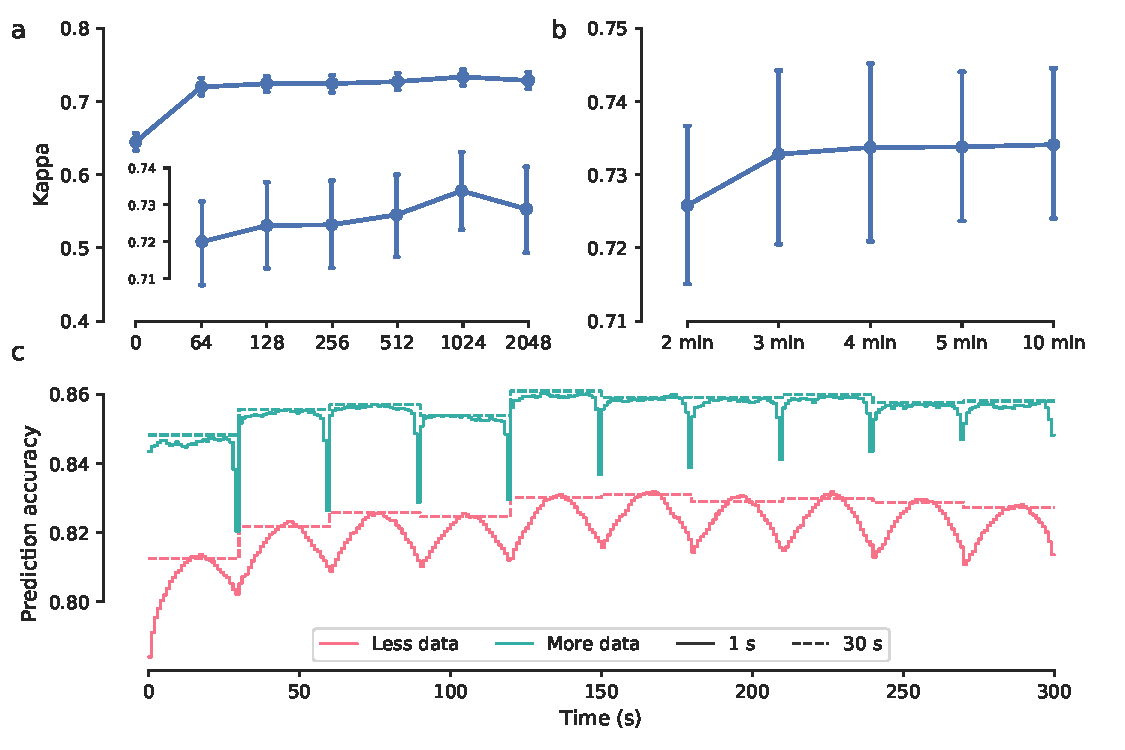
\includegraphics[width=\linewidth]{figures/paper-ii/figure_02_a-c.pdf}
    \caption[\acs{MASSC}v2 temporal context]{Temporal context changes model performance. a) Cohen's kappa as a function of the number of hidden units in the recurrent block. Inset shows zoom of Cohen's kappa for non-zero hidden unit values. b) Cohen's kappa as a function of sequence length. c) Prediction accuracy averaged across all 5-minute sequences in the test partition with a small and large training partition. Full lines are predictions evaluated every 1 s, while dashed lines show predictions averaged every 30 s. Values are shown for panels a), b) as mean with 95\% confidence intervals.}
    \label{fig:sleep-stages:paper-ii:figure-02}
\end{adjustwidth*}
\end{figure}

\subsection{Results}

In this section we report on the results of the three experiments described in~\cref{sec:sleep-stages:paper-ii:experimental-setup}.

\subsubsection{Temporal context impact on model performance}

% Please add the following required packages to your document preamble:
% \usepackage{booktabs}
\begin{table}[t]
\begin{adjustwidth*}{}{-\marginparwidth-0.5\marginparsep}
\begin{threeparttable}
\small
\caption[\acs{MASSC}v2 temporal context]{Temporal context impact on model performance in validation partition (\(n=426\)).}
\label{tab:sleep-stages:paper-ii:table-s01}
\begin{tabular}{@{}lcccccccc@{}}
\toprule
                         & \multicolumn{4}{c}{\textbf{Overall accuracy}}                         & \multicolumn{4}{c}{\textbf{Cohen’s kappa}}                            \\ \cline{2-9}
                         & \textbf{Mean} & \textbf{SD} & \textbf{Median} & \textbf{95\% CI} & \textbf{Mean} & \textbf{SD} & \textbf{Median} & \textbf{95\% CI} \\ \midrule
\textbf{Hidden units}    &               &             &                 &                       &               &             &                 &                       \\
\(\quad\)0                        & 0.779         & 0.083       & 0.794           & [0.771-0.787]         & 0.645         & 0.126       & 0.660           & [0.633-0.657]         \\
\(\quad\)64                       & 0.818         & 0.079       & 0.837           & [0.810-0.825]         & 0.720         & 0.120       & 0.745           & [0.709-0.731]         \\
\(\quad\)128                      & 0.821         & 0.080       & 0.841           & [0.813-0.829]         & 0.724         & 0.121       & 0.745           & [0.713-0.736]         \\
\(\quad\)256                      & 0.820         & 0.082       & 0.843           & [0.812-0.828]         & 0.725         & 0.124       & 0.751           & [0.713-0.736]         \\
\(\quad\)512                      & 0.822         & 0.079       & 0.841           & [0.815-0.830]         & 0.727         & 0.119       & 0.752           & [0.716-0.739]         \\
\(\quad\)1024                     & 0.828         & 0.072       & 0.845           & [0.821-0.835]         & 0.734         & 0.111       & 0.758           & [0.723-0.744]         \\
\(\quad\)2048                     & 0.823         & 0.080       & 0.843           & [0.816-0.831]         & 0.729         & 0.122       & 0.757           & [0.717-0.740]         \\
\textbf{Sequence length} &               &             &                 &                       &               &             &                 &                       \\
\(\quad\)2 min                    & 0.821         & 0.075       & 0.840           & [0.814-0.828]         & 0.726         & 0.114       & 0.754           & [0.715-0.737]         \\
\(\quad\)3 min                    & 0.826         & 0.080       & 0.845           & [0.818-0.833]         & 0.733         & 0.123       & 0.762           & [0.721-0.744]         \\
\(\quad\)4 min                    & 0.828         & 0.079       & 0.849           & [0.820-0.835]         & 0.734         & 0.122       & 0.762           & [0.722-0.745]         \\
\(\quad\)5 min                    & 0.828         & 0.072       & 0.845           & [0.821-0.835]         & 0.734         & 0.111       & 0.758           & [0.723-0.744]         \\
\(\quad\)10 min                   & 0.829         & 0.075       & 0.848           & [0.822-0.836]         & 0.734         & 0.113       & 0.759           & [0.723-0.745]         \\
\textbf{Window length}   &               &             &                 &                       &               &             &                 &                       \\
\(\quad\)1 s                      & 0.824         & 0.074       & 0.843           & [0.817-0.831]         & 0.728         & 0.113       & 0.752           & [0.717-0.738]         \\
\(\quad\)3 s                      & 0.824         & 0.074       & 0.845           & [0.817-0.832]         & 0.728         & 0.113       & 0.752           & [0.717-0.739]         \\
\(\quad\)5 s                      & 0.825         & 0.074       & 0.843           & [0.818-0.832]         & 0.728         & 0.113       & 0.752           & [0.717-0.739]         \\
\(\quad\)10 s                     & 0.825         & 0.074       & 0.844           & [0.818-0.832]         & 0.729         & 0.113       & 0.753           & [0.718-0.739]         \\
\(\quad\)15 s                     & 0.826         & 0.074       & 0.845           & [0.818-0.833]         & 0.729         & 0.113       & 0.755           & [0.719-0.740]         \\
\(\quad\)30 s                     & 0.829         & 0.075       & 0.848           & [0.822-0.836]         & 0.734         & 0.113       & 0.759           & [0.723-0.745]         \\ \bottomrule
\end{tabular}
\begin{tablenotes}
\small \item The hidden units variable corresponds to varying the complexity in the recurrent module by increasing the number of hidden units. Sequence length indicate the length of the sequence of 30 epochs, while window length correspond to varying the evaluation frequency. Means, standard deviations (SD) and medians are based on performance for each \ac{PSG}.
\end{tablenotes}
\end{threeparttable}
\end{adjustwidth*}
\end{table}

In~\cref{fig:sleep-stages:paper-ii:figure-02} we show how the model performance depends on the temporal context and complexity of the temporal processing module, when evaluating the model on the validation partition.
Results are further detailed in~\cref{tab:sleep-stages:paper-ii:table-s01}.
Specifically, we observe a drastic change in \cohen just by introducing a simple recurrent unit into the network as shown in~\cref{fig:sleep-stages:paper-ii:figure-02}a, where \cohen increases from \ci{0.645}{0.126}{0.633}{0.657} at $n_h=0$ to \ci{0.720}{0.120}{0.709}{0.731} at $n_h=64$. 
We did not observe any major changes when increasing the number of hidden units beyond $n_h=64$, although we did see a maximum \cohen of \ci{0.734}{0.111}{0.723}{0.744} at $n_h=1024$, which is shown in the inset in~\cref{fig:sleep-stages:paper-ii:figure-02}a. 
We observed a general increase in \cohen when classifying longer sequences than \SI{2}{\minute} (\ci{0.726}{0.114}{0.715}{0.737}), but did not see any major differences when classifying over more than \SI{3}{\minute} sequences (\ci{0.733}{0.123}{0.721}{0.7444}).
Subsequent models were fixed with $n_h=1024$ corresponding to a sequence length of \SI{5}{\minute}.

\subsubsection{Model classifications converge to 30 s predictions given sufficient training data}
Furthermore, we analyzed the classification performance of the model given a specific sequence length by looking at the average prediction accuracy across all \SI{5}{\minute} sequences in all subject \acp{PSG} in the test partition, similar to what~\citeauthor{Brink-Kjaer2019} has shown previously~\cite{Brink-Kjaer2019}.
In~\cref{fig:sleep-stages:paper-ii:figure-02}c, we show how the average classification accuracy in a \SI{5}{\minute} sequence both depends on the amount of data and the frequency of evaluating the model output, \ie every \SI{1}{\second} or across \SI{30}{\second}.
The average classification accuracy was found to be slightly lower in the beginning of each \SI{5}{\minute} sequence, both when training a model with less (500 training subjects) and more (\SI{75}{\percent} of total training subjects).
Interestingly, when training with less data, we also observed a lower accuracy in the beginning and end of each \SI{30}{\second} segment relative to the accuracy in the middle section, which was not the case when training with more data.

\subsubsection{Choice of cohort impacts classification performance on test set}

\begin{figure}[tb]
    % \centering
    \begin{adjustwidth*}{}{-\marginparwidth-\marginparsep}
    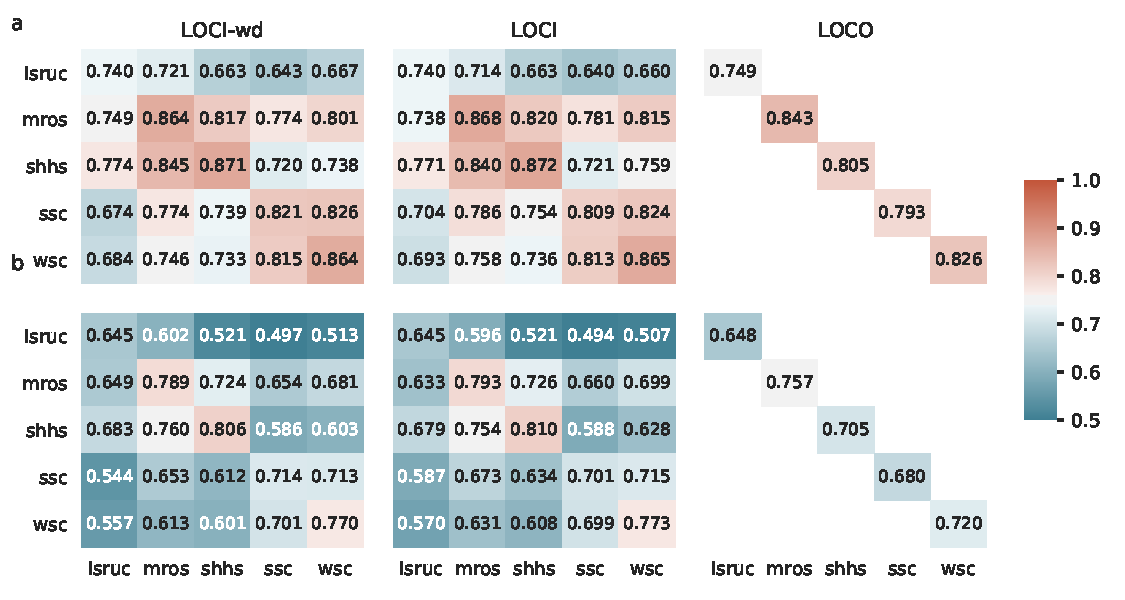
\includegraphics[width=\linewidth]{figures/paper-ii/figure_03_a-b.pdf}
    % 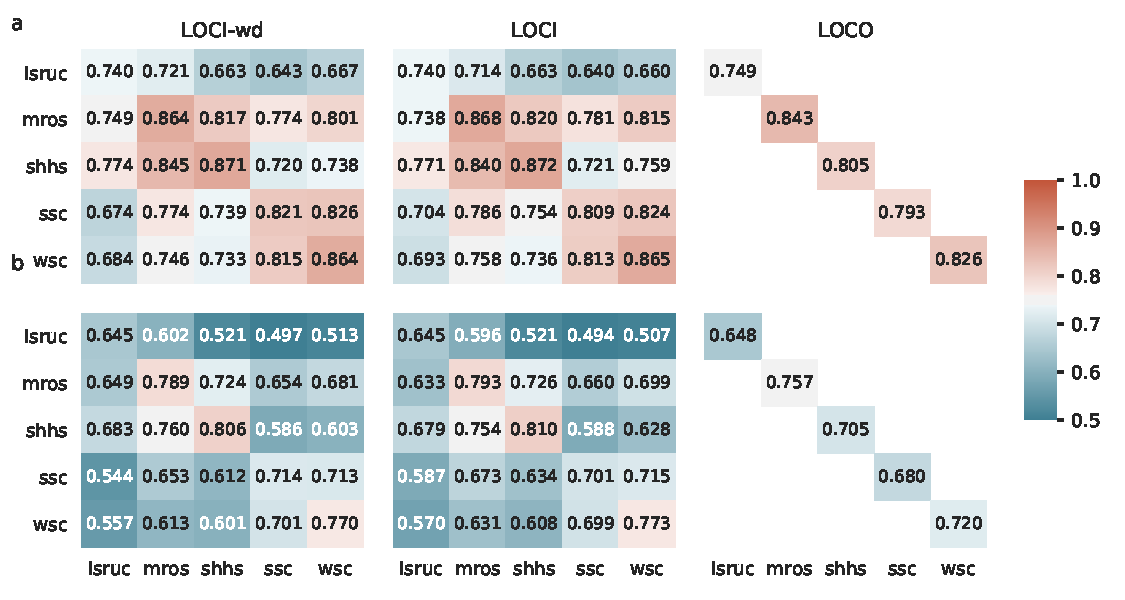
\includegraphics[width=\textwidth+\marginparwidth+\marginparsep]{figures/paper-ii/figure_03_a-b.pdf}
    \caption[\acs{MASSC}v2 \acs{LOCI} and \acs{LOCO} performance]{Individual cohorts influence classification performance on test partition \((N=1,584)\). As an example, training on \ac{MrOS} in a \ac{LOCI} configuration, the performance on the test subset of \ac{WSC} is 0.815. The diagonals in all three configurations shows the performance for the same subjects in the test subsets in the respective cohorts making possible direct comparisons between \ac{LOCI} and \ac{LOCO}. For aggregated metrics and more summary statistics, please see Table 4. %
    \describe{LOCI}; %
    \acs{LOCI}-wd: \acs{LOCI} with weight decay; %
    \describe{LOCO}; %
    \describe{ISRUC}; %
    \describe{MrOS}; % 
    \describe{SHHS}; %
    \describe{SSC}; %
    \describe{WSC}.}
    \label{fig:sleep-stages:paper-ii:figure-03}
    \end{adjustwidth*}
\end{figure}
\begin{figure}[tb]
    % \centering
    \begin{adjustwidth*}{}{-\marginparwidth-\marginparsep}
    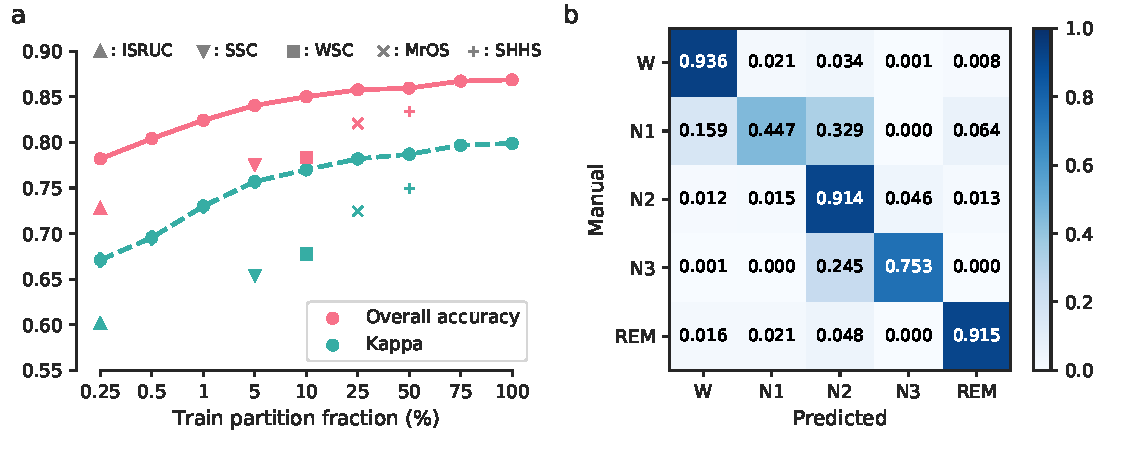
\includegraphics[width=\linewidth]{figures/paper-ii/figure_04_a-b.pdf}
    \caption[\acs{MASSC}v2 training on mixed data.]{Training on mixed data increased predictive performance compared to individual cohorts of similar size. a) There is a gain in predictive performance by mixing data from various sources consistent across the size of the training dataset. b) Confusion matrix for a model trained on 100\% of the available training partition data. The model shows excellent performance overall, with most misclassification happening between \ac{W} and \ac{N1}, and \ac{N1}, \ac{N2}, and \ac{N3}. This is somewhat consistent with clinical experience, since \ac{N1} is a transition stage between wake and the deeper stages of sleep with much frequency content overlap with both \ac{W} and \ac{N2}.}
    \label{fig:sleep-stages:paper-ii:figure-04}
    \end{adjustwidth*}
\end{figure}

In~\cref{fig:sleep-stages:paper-ii:figure-03} we show how training on different cohorts yield differing results in subsequent testing performance, here expressed in heatmaps as both overall accuracy (\cref{fig:sleep-stages:paper-ii:figure-03}a), and \cohen (\cref{fig:sleep-stages:paper-ii:figure-03}b) averaged across all $N=1584$ subject \acp{PSG} in the test partition.
The first two columns show the performance on the cohort on the \textit{x}-axis, when training on the specific cohort on the \textit{y}-axis.
Since the training subset in \ac{ISRUC} is small compared to the other cohorts, we trained the models in the left-most column with weight decay of $10^{-4}$ to compensate for the risk of overfitting, however, by comparing the left and middle columns, we did not observe any specific gain in classification performance by doing so.
The right-most column shows the test performance for each cohort, when excluding that cohort from training.
We observe a significant spread in classification accuracy across the different cohorts with prediction on \ac{ISRUC} being poorest, while prediction on \ac{MrOS} data being best.
Further details can be found in~\cref{tab:sleep-stages:paper-ii:table-s02}.

\begin{table}[tb]
\begin{adjustwidth*}{}{-\marginparwidth-0.5\marginparsep}
\begin{threeparttable}
\footnotesize
\caption[\acs{MASSC}v2 performance for \acs{LOCI} and \acs{LOCO}.]{Performance characteristics for \acs{LOCI} and \acs{LOCO} training configurations.}
\label{tab:sleep-stages:paper-ii:table-s02}
\begin{tabular}{@{}lccccccccc@{}}
\toprule
                 &                 & \multicolumn{4}{c}{\textbf{Overall accuracy}}                         & \multicolumn{4}{c}{\textbf{Cohen’s kappa}}                            \\ \cline{3-10}
                 & \textbf{N PSGs} & \textbf{Mean} & \textbf{SD} & \textbf{Median} & \textbf{95\% CI, mean} & \textbf{Mean} & \textbf{SD} & \textbf{Median} & \textbf{95\% CI, mean} \\ \midrule
\textbf{LOCI-wd} &                 &               &             &                 &                       &               &             &                 &                       \\
\(\quad\)\acs{ISRUC}            & 1584            & 0.679         & 0.123       & 0.701           & [0.673-0.685]         & 0.542         & 0.169       & 0.574           & [0.533-0.550]         \\
\(\quad\)\acs{MrOS}             & 1584            & 0.821         & 0.077       & 0.835           & [0.817-0.825]         & 0.727         & 0.114       & 0.745           & [0.721-0.733]         \\
\(\quad\)\acs{SHHS}             & 1584            & 0.834         & 0.088       & 0.858           & [0.830-0.839]         & 0.750         & 0.132       & 0.786           & [0.744-0.757]         \\
\(\quad\)\acs{SHHS}              & 1584            & 0.762         & 0.094       & 0.774           & [0.757-0.767]         & 0.639         & 0.129       & 0.654           & [0.633-0.646]         \\
\(\quad\)\acs{WSC}              & 1584            & 0.758         & 0.105       & 0.773           & [0.753-0.764]         & 0.633         & 0.145       & 0.653           & [0.626-0.640]         \\
\textbf{LOCI}    &                 &               &             &                 &                       &               &             &                 &                       \\
\(\quad\)\acs{ISRUC}            & 1584            & 0.676         & 0.124       & 0.700           & [0.670-0.682]         & 0.539         & 0.170       & 0.574           & [0.531-0.547]         \\
\(\quad\)\acs{MrOS}             & 1584            & 0.826         & 0.074       & 0.839           & [0.822-0.829]         & 0.732         & 0.111       & 0.748           & [0.726-0.737]         \\
\(\quad\)\acs{SHHS}\(^{\ddagger}\)            & 1584            & 0.837         & 0.084       & 0.858           & [0.833-0.841]         & 0.754         & 0.127       & 0.786           & [0.748-0.761]         \\
\(\quad\)\acs{SHHS}              & 1584            & 0.773         & 0.088       & 0.785           & [0.769-0.777]         & 0.657         & 0.125       & 0.671           & [0.651-0.663]         \\
\(\quad\)\acs{WSC}              & 1584            & 0.763         & 0.101       & 0.776           & [0.758-0.768]         & 0.641         & 0.140       & 0.659           & [0.635-0.648]         \\
\textbf{LOCO}    &                 &               &             &                 &                       &               &             &                 &                       \\
\(\quad\)\acs{ISRUC}\(^{\dagger}\)           & 52              & 0.749         & 0.081       & 0.764           & [0.727-0.771]         & 0.648         & 0.119       & 0.682           & [0.616-0.680]         \\
                 & 126             & 0.757         & 0.071       & 0.766           & [0.744-0.769]         & 0.661         & 0.101       & 0.682           & [0.643-0.678]         \\
\(\quad\)\acs{MrOS}\(^{\dagger}\)            & 371             & 0.843         & 0.066       & 0.851           & [0.836-0.849]         & 0.757         & 0.104       & 0.776           & [0.746-0.767]         \\
                 & 3932            & 0.841         & 0.069       & 0.854           & [0.838-0.843]         & 0.752         & 0.107       & 0.775           & [0.749-0.755]         \\
\(\quad\)\acs{SHHS}             & 846             & 0.805         & 0.076       & 0.815           & [0.800-0.810]         & 0.705         & 0.109       & 0.722           & [0.698-0.712]         \\
                 & 8444            & 0.800         & 0.081       & 0.811           & [0.798-0.801]         & 0.697         & 0.115       & 0.713           & [0.694-0.699]         \\
\(\quad\)\acs{SHHS}              & 76              & 0.793         & 0.086       & 0.809           & [0.744-0.812]         & 0.680         & 0.120       & 0.700           & [0.653-0.707]         \\
                 & 766             & 0.798         & 0.086       & 0.815           & [0.792-0.805]         & 0.690         & 0.123       & 0.711           & [0.681-0.699]         \\
\(\quad\)\acs{WSC}\(^{\dagger}\)             & 239             & 0.826         & 0.065       & 0.835           & [0.818-0.834]         & 0.720         & 0.096       & 0.736           & [0.708-0.732]         \\
                 & 2411            & 0.824         & 0.068       & 0.837           & [0.821-0.827]         & 0.718         & 0.100       & 0.736           & [0.714-0.722]         \\ \bottomrule
\end{tabular}
\begin{tablenotes}
\small \item Metrics are aggregated across all subjects for each cohort in test partition (\(N=1584\) \acp{PSG}). 
Bottom rows in \ac{LOCO} configuration correspond to evaluating performance on entire cohort. 
\describe{PSG}; %
\describe{LOCI}; %
\acs{LOCI}-wd: \acs{LOCI} with weight decay; %
\describe{LOCO}; %
\describe{ISRUC}; %
\describe{MrOS}; %
\describe{SHHS}; %
\describe{SSC}; %
\describe{WSC}; %
\(^{\dagger}\)significantly better than corresponding \ac{LOCI}; %
\(^{\ddagger}\)significantly better than corresponding \ac{LOCO}.
\end{tablenotes}
\end{threeparttable}
\end{adjustwidth*}
\end{table}

\subsubsection{More data is good, diverse data is better}

We observed a general increase in classification performance both in terms of overall accuracy and \cohen, when including more data in the model training phase in both the mixed- and single-cohort setting (\cref{fig:sleep-stages:paper-ii:figure-04}a,~\cref{tab:sleep-stages:paper-ii:table-s03}).
Classification performance was consistently lower in the single-cohort setting compared to the corresponding mixed-cohort setting. 
Interestingly, we found that training a model with just \SI{0.25}{\percent} of mixed-cohort training data still achieved an acceptable accuracy comparable to training a model with only \ac{SHHS} data, while using all available training data increased that performance by almost 10 percentage points.
Furthermore, we observed that the model trained with \SI{100}{\percent} of the training partition reached a state-of-the-art level of performance with an overall accuracy of \ci{0.869}{0.064}{0.865}{0.872} and \cohen of \ci{0.799}{0.098}{0.794}{0.804} (\cref{tab:sleep-stages:paper-ii:table-s03}).
The model furthermore performs well with respect to classifying individual sleep stages as shown in the confusion matrix in~\cref{fig:sleep-stages:paper-ii:figure-04}b.
However, the model still has difficulties classifying and distinguishing between certain sleep stages, especially between \ac{N2}, \ac{N1}, and \ac{N3}; and \ac{W}, \ac{N2}, and \ac{N1}.

\begin{table}[tb]
\begin{adjustwidth*}{}{-\marginparwidth-0.25\marginparsep}
\begin{threeparttable}
\small
\caption[\acs{MASSC}v2 performance for fractions of data.]{Model performance of test partition with varying fractions of training data.}
\label{tab:sleep-stages:paper-ii:table-s03}
\begin{tabular}{@{}lcccccccc@{}}
\toprule
                      & \multicolumn{4}{c}{\textbf{Overall accuracy}}                         & \multicolumn{4}{c}{\textbf{Cohen’s kappa}}                            \\ \cline{2-9}
\textbf{Fraction, \%} & \textbf{Mean} & \textbf{SD} & \textbf{Median} & \textbf{95\% CI, mean} & \textbf{Mean} & \textbf{SD} & \textbf{Median} & \textbf{95\% CI, mean} \\ \midrule
\(\quad\)0.25                  & 0.782         & 0.097       & 0.801           & [0.777-0.787]         & 0.671         & 0.141       & 0.696           & [0.664-0.678]         \\
\(\quad\)0.50                  & 0.804         & 0.086       & 0.824           & [0.800-0.808]         & 0.696         & 0.131       & 0.724           & [0.689-0.702]         \\
\(\quad\)1                     & 0.824         & 0.079       & 0.840           & [0.820-0.828]         & 0.730         & 0.118       & 0.753           & [0.724-0.736]         \\
\(\quad\)5                     & 0.841         & 0.074       & 0.856           & [0.837-0.844]         & 0.757         & 0.113       & 0.780           & [0.751-0.763]         \\
\(\quad\)10                    & 0.850         & 0.069       & 0.864           & [0.847-0.853]         & 0.770         & 0.108       & 0.791           & [0.765-0.775]         \\
\(\quad\)25                    & 0.858         & 0.066       & 0.873           & [0.854-0.861]         & 0.782         & 0.102       & 0.804           & [0.777-0.787]         \\
\(\quad\)50                    & 0.860         & 0.063       & 0.874           & [0.856-0.863]         & 0.787         & 0.097       & 0.809           & [0.782-0.792]         \\
\(\quad\)75                    & 0.867         & 0.062       & 0.882           & [0.864-0.870]         & 0.797         & 0.096       & 0.818           & [0.792-0.802]         \\
\(\quad\)100                   & 0.869         & 0.064       & 0.883           & [0.865-0.872]         & 0.799         & 0.098       & 0.820           & [0.794-0.804]         \\ \bottomrule
\end{tabular}
\begin{tablenotes}
\small \item Increasing the available training data increased performance on the test partition (\(N=1584\)) shown here as aggregated metrics across all subjects. No statistical difference was found by comparing confidence intervals between models trained with 75\% and 100\% of available training data, which indicates a saturation in training.
\end{tablenotes}
\end{threeparttable}
\end{adjustwidth*}
\end{table}

\subsubsection{Increasing the number of data sources improves classification performance}

\begin{figure}[tb]
    \centering
    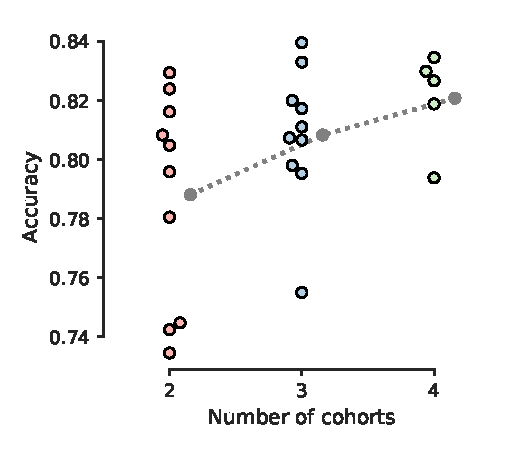
\includegraphics[width=0.75\columnwidth]{figures/paper-ii/figure_05.pdf}
    \caption[\acs{MASSC}v2 number of cohorts increases performance]{Number of cohorts in training partition increases model performance. Each datapoint is shown as the overall accuracy aggregated across all subjects for a specific training configuration. For example, the bottom dot in column 2 (3 cohort configuration) shows the performance on the test set (overall accuracy \ci{0.755}{0.109}{0.750}{0.760}), when training with 500 PSGs randomly and evenly drawn from \ac{SSC}, \ac{ISRUC}, and \ac{WSC}. Notice the scale on the \(y\)-axis.}
    \label{fig:sleep-stages:paper-ii:figure-05}
\end{figure}

On average, we saw an increase in overall accuracy, when increasing the number of cohorts from 2 to 4 using 500 \acp{PSG} in each configuration, see~\cref{fig:sleep-stages:paper-ii:figure-05} and~\cref{tab:sleep-stages:paper-ii:table-s04}.
Specifically, we found that the average overall accuracy increased from \ci{0.788}{0.102}{0.787}{0.790} in the 2-cohort configuration to \ci{0.808}{0.092}{0.807}{0.810} and \ci{0.821}{0.085}{0.819}{0.823} in the 3- and 4-cohort configurations, respectively.

\begin{table}
\begin{adjustwidth*}{}{-\marginparwidth-\marginparsep}
\begin{threeparttable}
\footnotesize
\caption[\acs{MASSC}v2 test performance.]{Model performance on test partition (\(N=1584\)) with varying number of cohorts in training partition.}
\label{tab:sleep-stages:paper-ii:table-s04}
\begin{tabular}{@{}lcccccccc@{}}
\toprule
                          & \multicolumn{4}{c}{\textbf{Overall accuracy}}                         & \multicolumn{4}{c}{\textbf{Kappa}}                                    \\ \cline{2-9}
\textbf{Training cohorts} & \textbf{Mean} & \textbf{SD} & \textbf{Median} & \textbf{95\% CI, mean} & \textbf{Mean} & \textbf{SD} & \textbf{Median} & \textbf{95\% CI, mean} \\ \midrule
\textbf{2}                &               &             &                 &                       &               &             &                 &                       \\
\textbf{Overall}          & 0.788         & 0.102       & 0.811           & [0.787-0.790]         & 0.683         & 0.143       & 0.710           & [0.681-0.685]         \\
\acs{ISRUC}-\acs{MrOS}                & 0.781         & 0.102       & 0.804           & [0.776-0.786]         & 0.675         & 0.143       & 0.703           & [0.668-0.682]         \\
\acs{ISRUC}-\acs{SHHS}                & 0.808         & 0.097       & 0.835           & [0.804-0.813]         & 0.717         & 0.142       & 0.756           & [0.710-0.724]         \\
\acs{ISRUC}-\acs{SSC}                 & 0.735         & 0.103       & 0.753           & [0.729-0.740]         & 0.613         & 0.140       & 0.638           & [0.606-0.620]         \\
\acs{ISRUC}-\acs{WSC}                 & 0.745         & 0.107       & 0.758           & [0.740-0.750]         & 0.628         & 0.140       & 0.642           & [0.621-0.635]         \\
\acs{MrOS}-\acs{SHHS}                 & 0.829         & 0.081       & 0.849           & [0.825-0.833]         & 0.740         & 0.124       & 0.769           & [0.734-0.746]         \\
\acs{MrOS}-\acs{SSC}                  & 0.796         & 0.090       & 0.816           & [0.791-0.800]         & 0.683         & 0.133       & 0.708           & [0.677-0.690]         \\
\acs{MrOS}-\acs{WSC}                  & 0.805         & 0.087       & 0.822           & [0.801-0.809]         & 0.699         & 0.126       & 0.722           & [0.693-0.705]         \\
\acs{SHHS}-\acs{SSC}                  & 0.816         & 0.090       & 0.839           & [0.812-0.821]         & 0.722         & 0.129       & 0.755           & [0.716-0.729]         \\
\acs{SHHS}-\acs{WSC}                  & 0.824         & 0.089       & 0.846           & [0.820-0.828]         & 0.733         & 0.128       & 0.762           & [0.727-0.739]         \\
\acs{SSC}-\acs{WSC}                   & 0.742         & 0.110       & 0.755           & [0.737-0.748]         & 0.620         & 0.145       & 0.634           & [0.613-0.627]         \\
\textbf{3}                &               &             &                 &                       &               &             &                 &                       \\
\textbf{Overall}          & 0.808         & 0.092       & 0.830           & [0.807-0.810]         & 0.711         & 0.131       & 0.739           & [0.709-0.713]         \\
\acs{ISRUC}-\acs{MrOS}-\acs{SHHS}           & 0.820         & 0.092       & 0.844           & [0.815-0.825]         & 0.732         & 0.134       & 0.766           & [0.725-0.738]         \\
\acs{ISRUC}-\acs{MrOS}-\acs{SSC}            & 0.798         & 0.088       & 0.816           & [0.794-0.802]         & 0.694         & 0.129       & 0.720           & [0.688-0.700]         \\
\acs{ISRUC}-\acs{MrOS}-\acs{WSC}            & 0.811         & 0.083       & 0.828           & [0.807-0.815]         & 0.711         & 0.119       & 0.735           & [0.705-0.717]         \\
\acs{ISRUC}-\acs{SHHS}-\acs{SSC}            & 0.807         & 0.090       & 0.828           & [0.803-0.812]         & 0.714         & 0.126       & 0.739           & [0.708-0.721]         \\
\acs{ISRUC}-\acs{SHHS}-\acs{WSC}            & 0.817         & 0.091       & 0.842           & [0.813-0.822]         & 0.728         & 0.128       & 0.759           & [0.722-0.735]         \\
\acs{ISRUC}-\acs{SSC}-\acs{WSC}             & 0.755         & 0.109       & 0.775           & [0.750-0.760]         & 0.639         & 0.150       & 0.670           & [0.631-0.646]         \\
\acs{MrOS}-\acs{SHHS}-\acs{SSC}             & 0.833         & 0.071       & 0.848           & [0.829-0.837]         & 0.744         & 0.109       & 0.766           & [0.739-0.750]         \\
\acs{MrOS}-\acs{SHHS}-\acs{WSC}             & 0.840         & 0.073       & 0.854           & [0.836-0.843]         & 0.753         & 0.109       & 0.774           & [0.748-0.759]         \\
\acs{MrOS}-\acs{SSC}-\acs{WSC}              & 0.795         & 0.088       & 0.811           & [0.791-0.800]         & 0.687         & 0.123       & 0.706           & [0.681-0.693]         \\
\acs{SHHS}-\acs{SSC}-\acs{WSC}              & 0.807         & 0.101       & 0.833           & [0.802-0.812]         & 0.710         & 0.142       & 0.744           & [0.703-0.717]         \\
\textbf{4}                &               &             &                 &                       &               &             &                 &                       \\
\textbf{Overall}          & 0.821         & 0.085       & 0.840           & [0.819-0.823]         & 0.728         & 0.124       & 0.755           & [0.726-0.731]         \\
\acs{ISRUC}-\acs{MrOS}-\acs{SHHS}-\acs{SSC}       & 0.827         & 0.078       & 0.843           & [0.823-0.831]         & 0.739         & 0.115       & 0.764           & [0.733-0.744]         \\
\acs{ISRUC}-\acs{MrOS}-\acs{SHHS}-\acs{WSC}       & 0.835         & 0.075       & 0.850           & [0.831-0.838]         & 0.747         & 0.112       & 0.768           & [0.742-0.753]         \\
\acs{ISRUC}-\acs{MrOS}-\acs{SSC}-\acs{WSC}        & 0.794         & 0.097       & 0.817           & [0.789-0.799]         & 0.687         & 0.139       & 0.716           & [0.680-0.694]         \\
\acs{ISRUC}-\acs{SHHS}-\acs{SSC}-\acs{WSC}        & 0.819         & 0.091       & 0.843           & [0.814-0.823]         & 0.728         & 0.131       & 0.759           & [0.721-0.734]         \\
\acs{MrOS}-\acs{SHHS}-\acs{SSC}-\acs{WSC}         & 0.830         & 0.076       & 0.846           & [0.826-0.834]         & 0.741         & 0.112       & 0.763           & [0.736-0.747]         \\ \bottomrule
\end{tabular}
\begin{tablenotes}
\small \item The total number of training records were fixed at \(N=500\) for all configurations. %
\describe{ISRUC}; %
\describe{MrOS}; %
\describe{SHHS}; %
\describe{SSC}; %
\describe{WSC}.
\end{tablenotes}
\end{threeparttable}
\end{adjustwidth*}
\end{table}

\subsection{Discussion}
In this work, we present an end-to-end deep learning-based model for fully automatic micro- and macro-sleep stage classification. 
Using all of the available data sources for training our model, we reached an overall accuracy on test partition of \ci{0.869}{0.064}{0.865}{0.872}, and a \cohen of \ci{0.799}{0.098}{0.794}{0.804}, which is in the very high end of the substantial agreement category for observer agreement~\cite{Landis1977}.
We found that individual cohorts exhibit major differences in overall accuracy and \cohen when subjected to both training and testing conditions and specifically, we found that average performance on the test partition in the \ac{LOCI} configurations varied significantly from \ci{0.676}{0.124}{0.670}{0.682} when training on \ac{ISRUC}, to \ci{0.837}{0.084}{0.833}{0.841} when training on \ac{SHHS}.
Each individual cohort also showed large deviations in predictive performance when tested on the other cohorts.
For example, when conditioned on \ac{SHHS} data, the lowest average accuracy was 0.721 on \ac{SSC} test data compared to the highest at 0.872 on \ac{SHHS} test data, while conditioning on \ac{SSC} training data, the lowest average accuracy was 0.704 on \ac{ISRUC} test data compared to 0.824 on \ac{WSC} test data.
Classification performance was generally higher on the test set when using the \ac{LOCO} configuration, except for \ac{SHHS} (higher in \ac{LOCI}) and \ac{SSC} (no difference).
We also found that having data from multiple sources always resulted in better-performing models compared to training on single cohorts.
Increasing the number of data sources increased classification performance, although this was non-significant.
In the design of the model, we observed that model performance was enhanced by the addition of the recurrent module (bGRU), a phenomenon likely reflecting the fact that sleep stage scoring at a specific time in one subject can be influenced by signal content (frequency, amplitude, presence of micro-events) at later time steps.
However, the complexity of the module given by the number of hidden units did not affect performance.
In all our experiments, we also evaluated the performance of the model every 1 s compared to the performance evaluated every 30 s and found them to be similar, which indicates the model is stable in classification in periods corresponding to an epoch of data.

Only a handful of studies have previously reported results when using multiple cohorts~\cite{Stephansen2018, Biswal2018, Patanaik2018}.
Some authors have reported a drop from 81.9\% to 77.7\% when training on the Massachusetts General Hospital cohort (MGH) and testing on MGH and \ac{SHHS}, respectively~\cite{Biswal2018}, while others have shown significant drops from 89.8\% to 81.4\% and 72.1\% on two separate hold-out sets from Singapore and USA~\cite{Patanaik2018}.
We also observed similar trends in our \ac{LOCI} and \ac{LOCO} experiments, where excluding the training subset of a cohort from the training partition resulted in a significant drop in performance on the respective test subset from that cohort.
A benefit of our \ac{LOCI} and \ac{LOCO} experiments is the possibility for direct benchmarking against previous publications using specific cohorts in their experiments.
For example, we obtain an accuracy of 0.805 in the \ac{LOCO}-\ac{SHHS} training-testing case compared to 0.777 previously reported by~\citeauthor{Biswal2018}~\cite{Biswal2018}, both of which reflect classification performance when \ac{SHHS} had not been used for training; and an accuracy of 0.865 in the \ac{LOCI}-\ac{WSC} case compared to 0.841 reported previously~\cite{Olesen2018c}, where both have been using a subset of \ac{WSC} for training the model. 
Interestingly, we obtained the same level of performance on the \ac{SHHS} data in our \ac{LOCI} experiment as reported by \citeauthor{Sors2018} (87\% accuracy, 81\% \cohen) even though they only used single-\ac{EEG} for their experiments~\cite{Sors2018}.
Other works that have investigated single- vs. multi-channel models for automatic sleep stage classification have found that models generally benefit from having more channels available for training~\cite{Chambon2018c, Biswal2018, Phan2019a}.
It may be that some cohorts share different characteristics that makes them more suitable for single- or multi-channel models, but this is speculative and would need to be verified in subsequent studies.

We only optimized our network architecture with respect to the temporal processing module and therefore cannot assess what impact different design choices for the other modules would have had on final performance.
For example, the \ac{EMG} signal has different statistical properties and spectral content, and separate, parallel architectures for \ac{EMG} and \ac{EEG}/ \ac{EOG} feature extraction may be warranted, as proposed by others~\cite{Chambon2018c, Stephansen2018}.
Other studies have however shown equal performance in large cohorts using a similar channel mixing approach as proposed here~\cite{Olesen2018c}.
Another limitation is found in our training runs, as we did not consider balancing our data with respect to the proportion of sleep stages, which may or may not have had impact on overall performance.
It is well established that there is significant variation in scoring and validation of \ac{N1}/\ac{REM} and \ac{N2}/\ac{N3}~\cite{Younes2016, Younes2018, Norman2000}, which challenges the training for any classification algorithm.
Some researchers have experimented balancing the cost of misclassifying sleep stages by weighting them by their inverse frequency of occurrence and found no significant improvement~\cite{Olesen2018c, Sors2018}, while others have experimented with balancing the sleep stage frequencies in each batch of data input to the neural network model~\cite{Chambon2018c}, but more rigorous research in resampling or over/under-sampling techniques is warranted in this regard.
We ultimately decided against experimenting with balancing our sleep stages in each batch, as we prioritized flexibility with regards to the length of input sequences fed to the network.
All our models ran through at least 50 epochs of training (passes through the training partition), which might have induced a bias in the configurations with larger cohorts.
For example, one pass through the training partition in the \ac{LOCI}-\ac{ISRUC} case corresponds to much less data than one pass through the \ac{LOCI}-\ac{SHHS} case.
However, since we selected the best performing model based on \cohen across all 50 epochs, we have allowed for more effective training in cases with less available training data.
We observed that models using less data in the training partition generally had to run for longer time (\ie more epochs) before converging.

In future studies on automatic sleep stage classification algorithms, we strongly recommend researchers to test and report results on not just hold-out test partitions, but also on cohorts completely unseen by the model both during training and testing/validation.
Our experiments indicate that even though good performance can be achieved on hold-out data using a single cohort, this does not necessarily translate into good generalization performance.
Such approach requires availability of many publicly available, high-quality, well-documented databases with easily accessible \ac{PSG} data, associated annotations and related patient information.
In this regard, websites such as the \ac{NSRR}, which contains several large databases with clinical data as well as \ac{PSG} and annotation data in a standardized format~\cite{Dean2016,Zhang2018}, are an invaluable resource for researchers. 
We also propose that the sleep science community establishes a common reference dataset on which researchers in machine learning can benchmark their models, similar to what the computer vision and general machine learning community has done with the ImageNet Large Scale Visual Recognition Challenge~\cite{Russakovsky2015}, an annual competition in which researchers submit their models to test in various competitions.

In summary, we have developed an automatic sleep stage classification algorithm based on deep learning, that can accurately classify sleep stages at a flexible resolution with a state-of-the-art classification performance of 87\% accuracy on a test set of 1584 \acp{PSG}.
We trained and tested our model using five cohorts with varying numbers of \acp{PSG} covering multiple phenotypes with specific focus on how well cohorts can generalize to each other.
We found that different cohorts generalize very differently both in intra- and inter-cohort settings (\ac{LOCI} vs. \ac{LOCO} experiments).
Furthermore, we also found that having more data sources significantly improve classification performance and generalizability to the extent that even just a small number of training \acp{PSG} can reach high classification performance by including many different sources.
To our knowledge, this is one of the largest, if not the largest, study on automatic sleep stage classification in terms of \ac{PSG} volume, diversity, and performance.

\clearpage\section{Paper III: Neural network analysis of sleep stages enables efficient diagnosis of narcolepsy}\label{sec:paperiii}
\sectionmark{Stephansen \& Olesen, \textit{et al.}, 2018}

\subsection{Materials \& Methods}
\begin{figure}[t]
    \myfloatalign   
    \subfloat[]
    {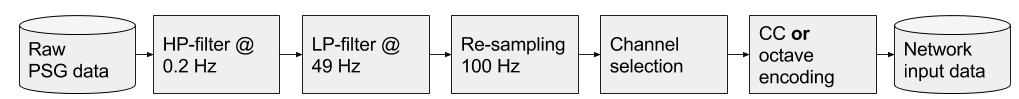
\includegraphics[width=\textwidth]{figures/paper-iii/Figure_5a.png}}  \\
    \subfloat[]
    {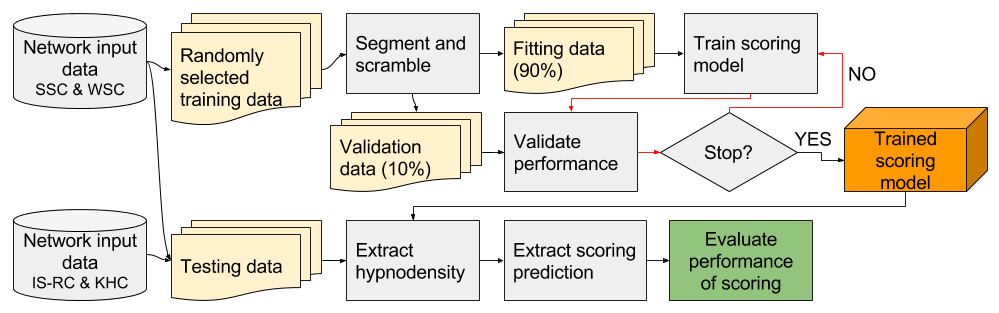
\includegraphics[width=\textwidth]{figures/paper-iii/Figure_5b.png}}
    \caption[STAGES model for sleep staging]{Overview of STAGES model for sleep stage classification. (a) Pre-processing steps taken to achieve the format of data as it is used in the neural networks. One of the 5 channels is first high-pass filtered with a cut-off at 0.2 Hz, then low-pass filtered with a cut-off at 49 Hz followed by a re-sampling to 100 Hz to ensure data homogeneity. In the case of EEG signals, a channel selection is employed to choose the channel with the least noise. The data are then encoded using either the CC or the octave encoding. (b) Steps taken to produce and test the automatic scoring algorithm. A part of the SSC10, 32 and WSC32, 33 is randomly selected, as described in~\cref{tab:paperiii-table01}. These data are then segmented in 5 min segments and scrambled with segments from other subjects to increase batch similarity during training. A neural network is then trained until convergence (evaluated using a separate validation sample). Once trained, the networks are tested on a separate part of the SSC and WSC along with data from the IS-RC31 and KHC10, 34.}
    \label{fig:paperiii-figure05}
\end{figure}
\subsubsection{Datasets}
The success of machine learning depends on the size and quality of the data on which the model is trained and evaluated~\cite{Banko2001, Shotton2011}.
We used a large dataset comprised of several thousand sleep studies to train, validate, and test/replicate our models.
To ensure significant heterogeneity, data came from 10 different cohorts recorded at 12 sleep centers across 3 continents: SSC~\cite{Andlauer2013, Moore2014}, WSC~\cite{Moore2014, Young2009a}, IS-RC~\cite{Kuna2013}, JCTS~\cite{InternationalXyremStudyGroup2005}, KHC~\cite{Hong2006}, AHC~\cite{Frauscher2013}, IHC~\cite{Pizza2015}, DHC~\cite{Christensen2017}, FHC, and CNC~\cite{Andlauer2012}.
Institutional Review Boards approved the study and informed consent was obtained from all participants.
Technicians trained in sleep scoring manually labeled all sleep studies.
Figure 5 a, b, and c summarize the overall design of the study for sleep stage scoring and narcolepsy biomarker development.
\Cref{tab:paperiii-table01} provides a summary of the size of each cohort and how it was used.
In the narcolepsy biomarker aspect of the study, PSGs from T1N and other patients were split across most datasets to ensure heterogeneity in both the training and testing dataset.
For this analysis, a few recordings with poor quality sleep studies, i.e. missing critical channels, with additional sensors or with a too short sleep duration ($\leq$ 2 hours) were excluded.
A “never seen” subset cohort that included French and Chinese subjects (FHC and CNC) was also tested.
Below is a brief description of each dataset.

\paragraph{Population-based Wisconsin Sleep Cohort}
This cohort is a longitudinal study of state agency employees aged 37 - 82 years from Wisconsin, and approximates a population-based sample (see~\cref{tab:paperiii-table01} for age at study) and are generally more overweight33.
The study is ongoing, and dates to 1988.
2167 PSGs in 1086 subjects were used for training while 286 randomly selected PSGs were used for validation testing of the sleep stage-scoring algorithm and narcolepsy biomarker training.
Approximately 25\% of the population have an Apnea Hypopnea Index (AHI) above 15/hour and 40\% have a PLMI above 15/hr.
A detailed description of the sample can be found in Young33 and Moore et al.32.
The sample does not contain any T1N patients, and the three subjects with possible T1N were removed54.

\paragraph{Patient-based Stanford Sleep Cohort}
PSGs from this cohort were recorded at the Stanford Sleep Clinic dating back to 1999, and represent sleep disorder patients aged 18-91 visiting the clinic (see~\cref{tab:paperiii-table01} for age at study).
The cohort contains thousands of PSG recordings, but for this study we used 894 diagnostic (no positive airway pressure (PAP)) recordings in independent patients that have been used in prior studies30.
This subset contains patients with a range of different diagnoses including: sleep disordered breathing (607), insomnia (141), REM sleep behavior disorder (4), restless legs syndrome (23), T1N (25), delayed sleep phase syndrome (14), and other conditions (39).
Description of the subsample can be found in Andlauer et al.10 and Moore et al.32.
Approximately 30\% of subjects have an AHI above 15/hour, or a PLMI above 15/hour.
617 randomly selected subjects were used for training the neural networks while 277 randomly selected PSGs were kept for validation testing of the sleep stage scoring algorithm.
These 277 subjects were also used for training the narcolepsy biomarker algorithm.
The sample contains PSGs of 25 independent untreated subjects with T1N (12 with low CSF hypocretin-1, the others with clear cataplexy).
26 subjects were removed from the study—4 due to poor data quality, and the rest because of medication use.

\paragraph{Patient-based Korean Hypersomnia Cohort}
The Korean Hypersomnia Cohort is a high pretest probability sample for narcolepsy.
It includes 160 patients with a primary complaint of excessive daytime sleepiness (see~\cref{tab:paperiii-table01} for age at study).
These PSGs were used for testing the sleep scoring algorithm and for training the narcolepsy biomarker algorithm.
No data was used for training the sleep-scoring algorithm.
Detailed description of the sample can be found in Hong et al.34 and Andlauer et al.10
The sample contains PSGs of 66 independent untreated subjects with T1N and clear cataplexy.
Two subjects were removed from the narcolepsy biomarker study because of poor data quality.

\paragraph{Patient-based Austrian Hypersomnia Cohort}
Patients in this cohort were examined at the Innsbruck Medical University in Austria as described in Frauscher et al.35.
The AHC contains 118 PSGs in 86 high pretest probability patients for narcolepsy (see~\cref{tab:paperiii-table01} for details).
42 patients (81 studies) are clear T1N with cataplexy cases, with all but 3 having a positive MSLT (these three subjects had a mean sleep latency (MSL)>8 minutes but multiple SOREMPs).
The rest of the sample has idiopathic hypersomnia and type 2 narcolepsy.
Four patients have an AHI>15/hour and 25 had a PLMI>15/hour.
Almost all subjects had two sleep recordings performed, which were kept together such that no two recordings from the same subject were split between training and testing partitions.

\paragraph{Patient-based Inter-scorer Reliability Cohort}
As Rosenberg et al.16 have shown, variation between individual scorers can sometimes be large, leading to an imprecise gold standard.
To quantify this, and to establish a more accurate gold standard, 10 scorers from five different institutions, University of Pennsylvania, St. Luke’s Hospital, University of Wisconsin at Madison, Harvard University, and Stanford University, analyzed the same 70 full night PSGs.
For this study, scoring data from University of Pennsylvania, St. Luke’s and Stanford were used.
All subjects are female (see~\cref{tab:paperiii-table01} for details).
This allowed for a much more precise gold standard, and the inter-scorer reliability could be quantified for a dataset, which could also be examined by automatic scoring algorithms.
Detailed description of the sample can be found in Kuna et al.31 and Malhotra6.
The sample does not contain any T1N patients.

\paragraph{The Jazz Clinical Trial Sample}
This sample includes seven baseline sleep PSGs from five sites taken from a clinical trial study of sodium oxybate in narcolepsy (SXB15 with 45 sites in Canada, USA, and Switzerland) conducted by Orphan Medical, now named Jazz Pharmaceuticals.
The few patients included are those with clear and frequent cataplexy (a requirement of the trial) that had no stimulant or antidepressant treatment at baseline43.
All 7 subjects in this sample were used exclusively for training the narcolepsy biomarker algorithm.

\paragraph{Patient-based Italian Hypersomnia Cohort}
Patients in this high pretest probability cohort (see~\cref{tab:paperiii-table01} for demographics) were examined at the IRCCS, Istituto delle Scienze Neurologiche ASL di Bologna in Italy as described in Pizza et al.41.
The IHC contains 70 \ntI patients (\SI{58}{\percent} male, \plusminus{29.5}{1.9} years old), with either documented low CSF hypocretin levels (59 cases, all but 2 HLA DQB1*06:02 positive), or clear cataplexy, positive MSLTs and HLA positivity (11 subjects).
As non-\ntI cases with unexplained daytime somnolence, the cohort includes 77 other patients: 19 with idiopathic hypersomnia, 7 with type 2 narcolepsy and normal CSF hypocretin-1, 48 with a subjective complaint of excessive daytime sleepiness not confirmed by MSLT, and 3 with secondary hypersomnia.
Subjects in this cohort were used for training (n=87) and testing (n=61) the narcolepsy biomarker algorithm. 

\paragraph{Patient-based Danish Hypersomnia Cohort}
Patients in this cohort were examined at the Rigshospitalet, Glostrup, Denmark as described in Christensen et al53.
The DHC contains 79 PSGs in controls and patients (see~\cref{tab:paperiii-table01} for details).
Based on PSG, multiple sleep latency test and cerebrospinal fluid hypocretin-1 measures, the cohort includes healthy controls (19 subjects), patients with other sleep disorders and excessive daytime sleepiness (20 patients with CSF hypocretin-1 $\geq$ 110 pg/ml), narcolepsy type 2 (22 patients with CSF hypocretin-1 $\geq$ 110 pg/ml), and T1N (28 patients with CSF hypocretin 1 $\leq$ 110 pg/ml).
All 79 subjects in this cohort were used exclusively for training the narcolepsy biomarker algorithm.

\paragraph{Patient-based French Hypersomnia Cohort}
This cohort consists of 122 individual PSGs recorded at the Sleep-Wake Disorders Center, Department of Neurology, Gui-de-Chauliac Hospital, CHU Montpellier, France (see~\cref{tab:paperiii-table01} for demographics).
The FHC contains 63 subjects with T1N (all but two tested with CSF hypocretin-1 $\leq$ 110 pg/ml, five below 18 years old, 55 tested for HLA, all positive for HLA DQB1*06:02) and 22 narcolepsy type 2 (19 with CSF hypocretin-1 > 200 pg/ml, and three subjects with CSF hypocretin-1 between 110 and 200 pg/ml, three HLA positive).
The remaining 36 subjects are controls (15 tested for HLA, two with DQB1*06:02) without other symptoms of hypersomnia.
The FHC was used as data for the replication study of the narcolepsy biomarker algorithm.

\paragraph{Patient-based Chinese Narcolepsy Cohort}
This cohort contains 199 individual PSGs recorded (see~\cref{tab:paperiii-table01} for demographics).
The CNC contains 67 subjects diagnosed with T1N exhibiting clear-cut cataplexy (55 tested HLA DQB1*06:02 positive), while the remaining 132 subjects are randomly selected population controls (15 HLA DQB1*06:02 positive, 34 HLA negative, remaining unknown) 12.
Together with the FHC, the CNC was used as data for the replication study of the narcolepsy biomarker algorithm.

\paragraph{American Academy of Sleep Medicine Sleep Study}
The AASM ISR dataset is composed of a single control sleep study of 150 30 sec epochs that was scored by \plusminus{5234}{14} experienced sleep technologists for quality control purposes.
Design of this dataset is described in Rosenberg et al.16.

\subsubsection{Data labels, scoring and fuzzy logic}
Sleep stages were scored by PSG-trained technicians using established scoring rules, as described in the AASM Scoring Manual7.
In doing so, technicians assign each epoch with a discrete value.
With a probabilistic model, like the one proposed in this study, a relationship to one of the fuzzy sets is inferred based on thousands of training examples labeled by many different scoring-technicians. 

The hypnodensity graph refers to the probability distribution over each possible stage for each epoch, as seen in Figure 2 a and b.
This allows more information to be conveyed, since every epoch of sleep within the same stage is not identical. For comparison with the gold standard, however, a discrete value must be assigned from the model output as:

\begin{equation}
    \hat{y} = \argmax_{\mathbf{y}_{i}} \sum_{i}^{N} \mathbf{P}_i \! \left( \mathbf{y}_i \! \mid \! \mathbf{x}_i \right),
\end{equation}
where $\mathbf{P}_i \! \left( \mathbf{y}_i \! \mid \! \mathbf{x}_i \right)$ is a vector with the estimated probabilities for each sleep stage in the \textit{i}th segment, $N$ is the number of segments an epoch is divided into, and $\hat{y}$ is the estimated label. 

Sleep scoring technicians score sleep in 30 second epochs, based on what stage they assess is represented in the majority of the epoch—a relic of when recordings were done on paper. This means that when multiple sleep stages are represented, more than half of the epoch may not match the assigned label. This is evident in the fact that the label accuracy decreases near transition epochs20. One solution to this problem is to remove transitional regions to purify each class. However, this has the disadvantage of under-sampling transitional stages, such as N1, and removes the context of quickly changing stages, as is found in a sudden arousal. It has been demonstrated that the negative effects of imperfect “noisy” labels may be mitigated if a large enough training dataset is incorporated and the model is robust to overfitting41. This also assumes that the noise is randomly distributed with an accurate mean—a bias cannot be cancelled out, regardless of the amount of training data. For these reasons, all data including those containing sleep transitions were included. Biases were evaluated by incorporating data from several different scoring experts cohorts and types of subjects.

To ensure quick convergence, while also allowing for long-term dependencies in memory-based models, the data were broken up in 5 minute blocks and shuffled to minimize the shift in covariates during training caused by differences between subjects. To quantify the importance of segment sizes, both 5 second and 15 second windows were also tested.

\begin{landscape}
\begin{table}
\begin{threeparttable}  
\centering
\small
\caption[STAGES cohorts]{Description of the various cohorts included in this study and how they were used.}
\label{tab:paperiii-table01}
\begin{tabular}{@{}lccccccccccc@{}}
    \toprule
    & & & & \multicolumn{2}{c}{Sleep scoring} & \multicolumn{3}{c}{Narcolepsy biomarker} & & & \\ \cline{5-6} \cline{7-9}
    Cohort         & Age, $ \mu \pm \sigma $        & BMI, $ \mu \pm \sigma $        & Sex, \% male       & Train      & Test      & Train  & Test              & Replication            & \% narco & \% hypersomnia \\ \midrule
    WSC            & 59.7 $ \pm $ 8.4  & 31.6 $ \pm $ 7.1  & 53.1      & 1086 (2167~PSGs) & 286  & 170                  & 116          & None        & 0        & 0 \\
    SSC            & 45.4 $ \pm $ 13.8 & 23.9 $ \pm $ 6.5  & 59.4      & 617                & 277  & 139                  & 112          & None        & 11.6     & 1.8 \\
    KHC            & 29.1 $ \pm $ 13.2 & 24.1 $ \pm $ 4.3  & 58.6      & None               & 160  & 87                   & 71           & None        & 45.8     & 54.2 \\
    AHC            & 34.5 $ \pm $ 13.8 & 25.9 $ \pm $ 4.9  & 54        & None               & None & 42 (76~PSGs)         & 44 (84~PSGs) & None        & 52.3     & 47.7 \\
    IS-RC          & 51.1 $ \pm $ 4.2  & 32.9 $ \pm $ 9.2  & 0         & None               & 70   & None                 & None         & None        & 0        & 0 \\
    JCTS           & 53.2 $ \pm $ 9.8  & 31.0 $ \pm $ 4.4  & 57.1      & None               & None & 7                    & None         & None        & 100      & 0 \\
    IHC            & 33.7 $ \pm $ 17.6 & -           & 56.7      & None               & None & 87                   & 61           & None        & 47.3     & 50 \\
    DHC            & 33.4 $ \pm $ 14.8 & 24.8 $ \pm $ 4.9  & 50        & None               & None & 79                   & None         & None        & 26.6     & 48.1 \\
    FHC            & 28.8 $ \pm $ 15.2 & 24.4 $ \pm $ 8.1  & 59        & None               & None & None                 & None         & 122         & 51.6     & 18 \\
    CNC            & 28.5 $ \pm $ 16.9 & 23.2 $ \pm $ 11.5 & 51.3      & None               & None & None                 & None         & 199         & 34.2     & 0 \\ \midrule
    Total subjects &             &             &           & 1,703              & 793  & 611                  & 404          & 321         &          & \\
    Total PSGs     &             &             &           & 2,784              & 793  & 645                  & 444          & 321         &          & \\ \bottomrule
\end{tabular}
\begin{tablenotes}
\footnotesize
\item WSC, SSC \quad Training and testing of sleep scoring models and narcolepsy biomarker.
\item KHC \quad Sleep scoring testing, and training and testing of narcolepsy biomarker.
\item AHC \quad Training and testing of narcolepsy biomarker. 86 subjects had the first PSG recorded, and 75 had an additional second PSG.\newline A subject was used for either training or testing.
\item IS-RC \quad Scored by 6 different scorers. Final assessment and validation of predictive performance for sleep scoring.
\item JCTS, DHC \quad Training of narcolepsy biomarker.
\item IHC \quad Training and testing of narcolepsy biomarker.
\item FHC, CNC \quad Replication of narcolepsy biomarker. 
\end{tablenotes}
\end{threeparttable}
\end{table}
\end{landscape}

\subsubsection{Data selection and pre-processing}
A full night PSG involves recording many different channels, some of which are not necessary for sleep scoring55. In this study, EEG – C3 or C4, and O1 or O2, chin EMG, and the left and right EOG channels were used, with reference to the contralateral mastoid. Poor electrode connections are common when performing a PSG analysis. This can lead to a noisy recording, rendering it useless. To determine whether right or left EEG channels were used, the noise of each was quantified by dividing the EEG data in 5 minute segments, and extracting the Hjorth parameters56. These were then log-transformed, averaged, and compared with a previously established multivariate distribution, based on the WSC32,33 and SSC10,32 training data. The channel with lowest Mahalanobis distance57 to this distribution was selected. The log-transformation has the advantage of making flat signals/disconnects as uncommon as very noisy signals, in turn making them less likely to be selected. To minimize heterogeneity across recordings, and at the same time reducing the size of the data, all channels were down-sampled to 100 Hz. Additionally, all channels were filtered with a 5th order two-direction infinite impulse response (IIR) high-pass filter with cutoff frequency of 0.2 Hz and a 5th order two-direction IIR low-pass filter with cutoff frequency of 49 Hz. The EMG signal contains frequencies well above 49 Hz, but since much data had been down-sampled to 100 Hz in the WSC, this cutoff was selected for all cohorts. All steps of the pre-processing are illustrated in Figure 5 a.

\subsubsection{Convolutional and recurrent neural networks}
Convolutional neural networks (CNN) are a class of deep learning models first developed to solve computer vision problems30. A CNN is a supervised classification model in which a low-level, such as an image, is transformed through a network of filters and sub-sampling layers. Each layer of filters produces a set of features from the previous layer, and as more layers are stacked, more complex features are generated. This network is coupled with a general-purpose learning algorithm, resulting in features produced by the model reflecting latent properties of the data rather than the imagination of the designer. This property places fewer constrictions on the model by allowing more flexibility, and hence the predictive power of the model will increase as more data is observed. This is facilitated by the large number of parameters in such a model, but may also necessitate a large amount of training data. Sleep stage scoring involves a classification of a discrete time-series, in which adjacent segments are correlated. Models that incorporate memory may take advantage of this and may lead to better overall performance by evening out fluctuations. However, these fluctuations may be the defining trait or anomaly of some underlying pathology (such as narcolepsy, a pathology well known to involve abnormal sleep stages transitions), present in only a fraction of subjects, and perhaps absent in the training data. This can be thought of similarly to a person with a speech impediment: the contextual information will ease the understanding, but knowing only the output, this might also hide the fact that the person has such a speech impediment. To analyze the importance of this, models with and without memory were analyzed. Memory can be added to such a model by introducing recurrent connections in the final layers of the model. This turns the model into a recurrent neural network (RNN). Classical RNNs had the problem of vanishing or exploding gradients, which meant that optimization was very difficult. This problem was solved by changing the configuration of the simple hidden node into a LSTM cell58. Models without this memory are referred to as FF models. A more in-depth explanation of CNNs including application areas can be found the review article on deep learning by LeCun, Bengio and Hinton30 and the deep learning textbook by Goodfellow, Bengio and Courville (2016)59. For a more general introduction to machine learning concepts, see the textbook by Bishop (2006)60.

\subsubsection{Data input and transformations}
Biophysical signals, such as those found in a PSG, inherently have a low signal to noise ratio, the degree of which varies between subjects, and hence learning robust features from these signals may be difficult. To circumvent this, two representations of the data that could minimize these effects were selected. An example of each decomposition is shown in~\cref{fig:paperiii-figure06}.

\begin{figure}[!tb]
    \myfloatalign   
    \subfloat[]
    {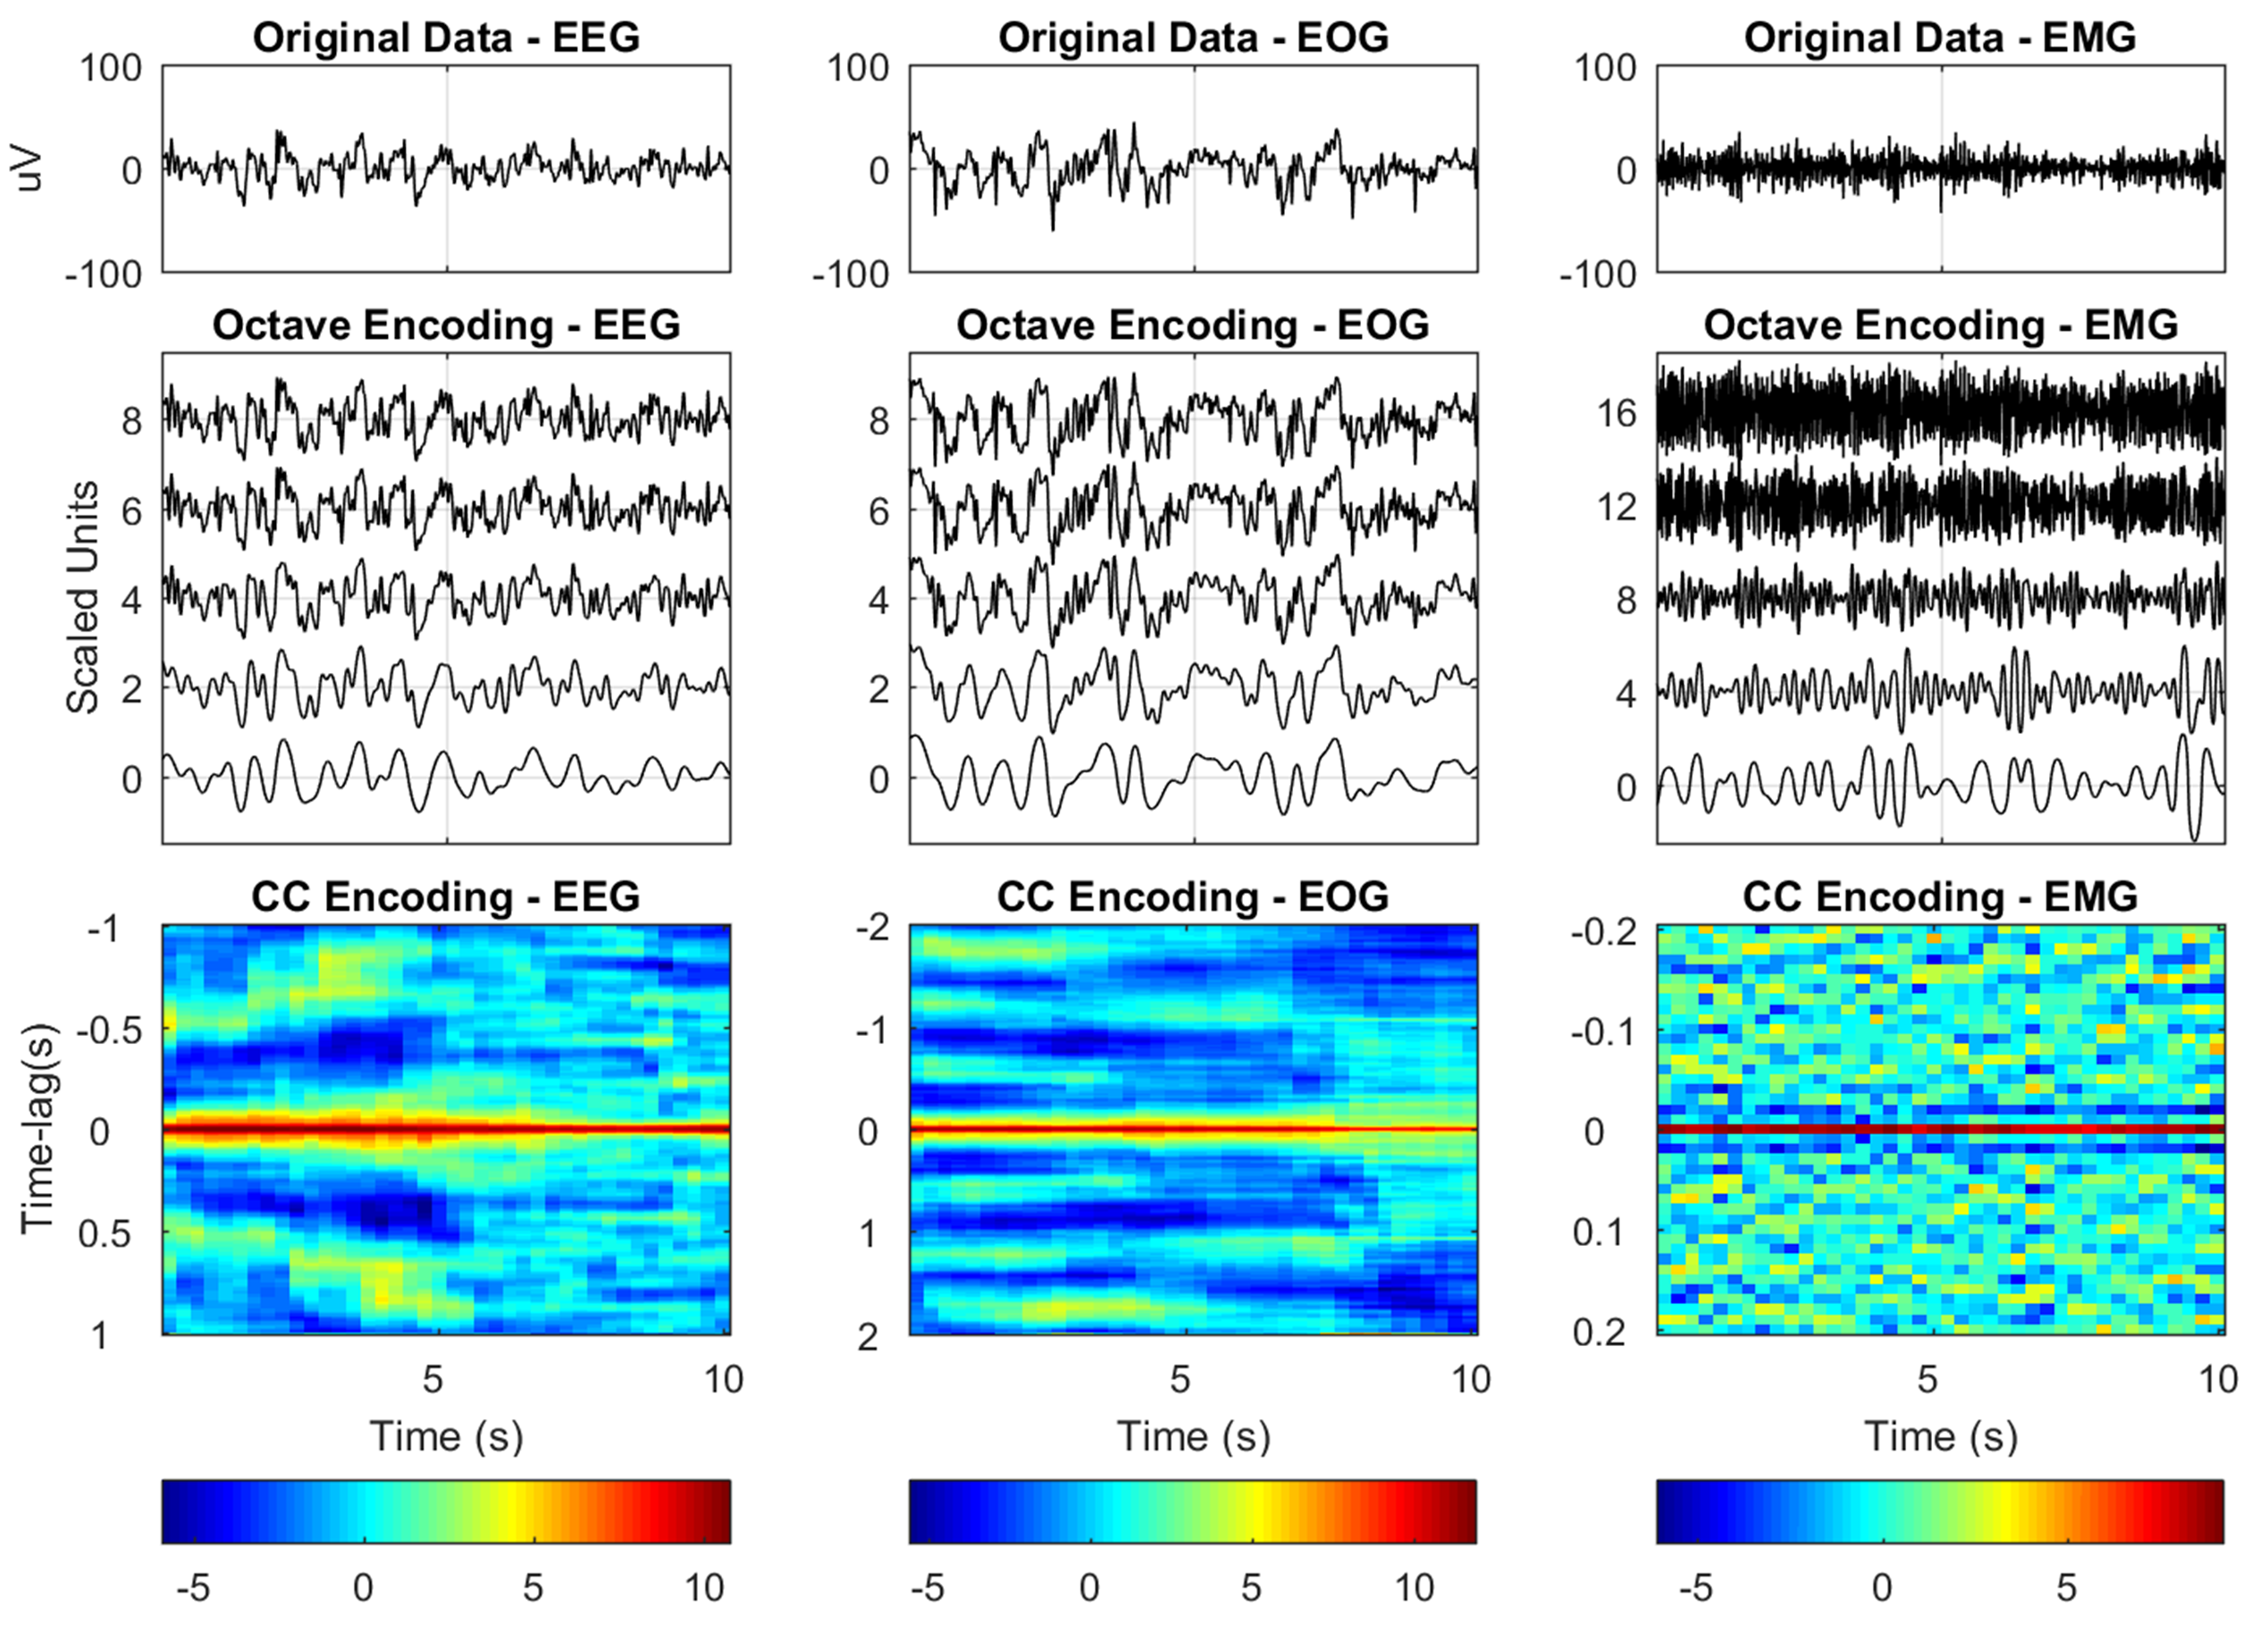
\includegraphics[width=\textwidth]{figures/paper-iii/ncomm_figure6a-2}}  \\
    \subfloat[]
    {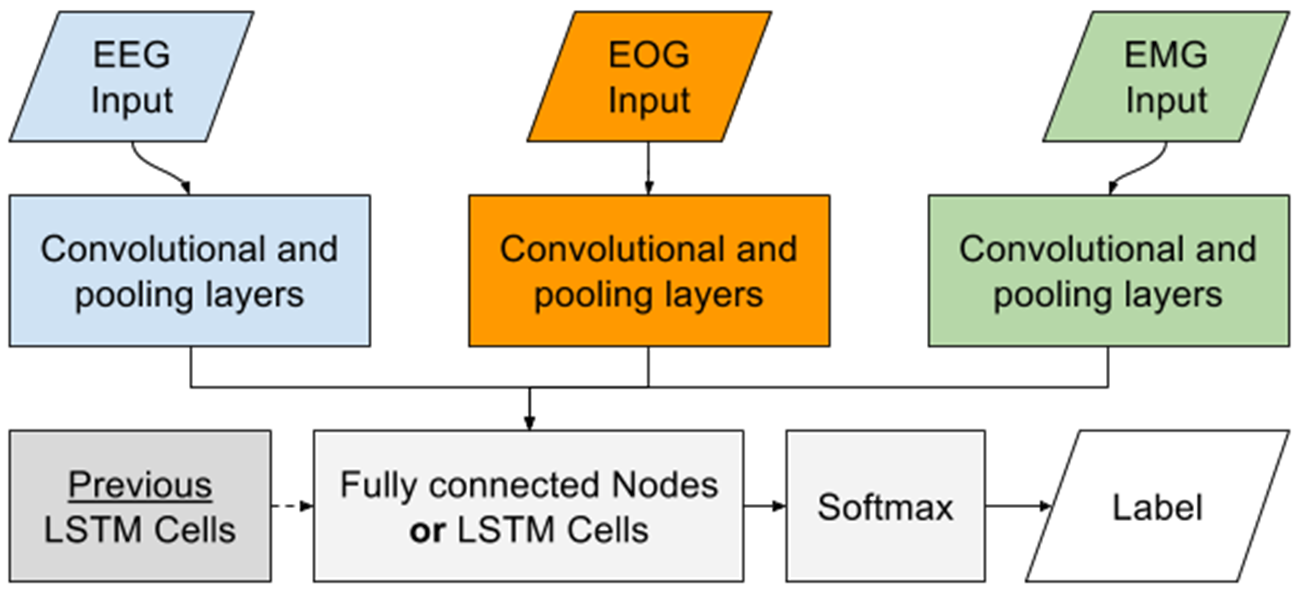
\includegraphics[width=0.7\textwidth]{figures/paper-iii/ncomm_figure6b-2}}
    \caption[Neural network strategy for STAGES model]{Neural network strategy for STAGES model. (a) An example of the octave and the CC encoding on 10 s of EEG, EOG and EMG data. These processed data are fed into the neural networks in one of the two formats. The data in the octave encoding are offset for visualization purposes. Color scale is unitless. (b) Simplified network configuration, displaying how data are fed and processed through the networks. A more detailed description of the network architecture is shown in~\cref{fig:paperiii-suppfigure03}.}
    \label{fig:paperiii-figure06}
\end{figure}

Octave encoding maintains all information in the signal, and enriches it by repeatedly removing the top half of the bandwidth (i.e. cut off frequencies of \SIlist{49;25;12.5;6.25;3.125}{\hertz}) using a series of low-pass filters, yielding a total of 5 new channels for each original channel. At no point is a high-pass filter applied. Instead, the high frequency information may be obtained by subtracting lower frequency channels —– an association the neural networks can make, given their universal approximator properties61. After filtration, each new channel is scaled to the 95th percentile and log modulus transformed:
\begin{equation}
    \mathbf{x}_{\mathrm{scaled}} = \sign \! \left( \mathbf{x} \right) \log{\left( \frac{|\mathbf{x}|}{p_{95}(\mathbf{x})} + 1 \right)}
\end{equation}
The initial scaling places 95\% of the data between -1 and 1, a range in which the log modulus is close to linear. Very large values, such as those found in particularly noisy areas, are attenuated greatly. Some recordings are noisy, making the \nth{95} percentile significantly higher than what the physiology reflects. Therefore, instead of the selecting the \nth{95} percentile from the entire recording, the recording is separated into 50\% overlapping 90 minute segments, from which the 95th percentile is extracted. The mode of these values is then used as a scaling reference. In general, scaling and normalization is important to ensure quick convergence as well as generalization in neural networks. The decomposition is done in the same way on every channel, resulting in 25 new channels in total.

Using a cross-correlation function, underlying periodicities in the data are revealed while noise is attenuated. White noise is by definition uncorrelated; its autocorrelation function is zero everywhere except lag zero. It is this property that is utilized, even though noise cannot always be modeled as such. PSG signals are often obscured by undesired noise that is uncorrelated with other aspects of the signals. An example CC between a signal segment and an extended version of the same signal segment is shown in~\cref{fig:paperiii-suppfigure05}. Choosing the CC in this manner over a standard autocorrelation function serves two purposes: the slow frequencies are expressed better, since there is always full overlap between the two signals (some of this can be adjusted with the normal autocorrelation function using an unbiased estimate); and the change in fluctuations over time within a segment is expressed, making the function reflect aspects of stationarity. Because this is the CC between a signal and an extended version of itself, the zero lag represents the power of that segment, as is the case in an autocorrelation function.
\begin{figure}[tb]
    \centering
    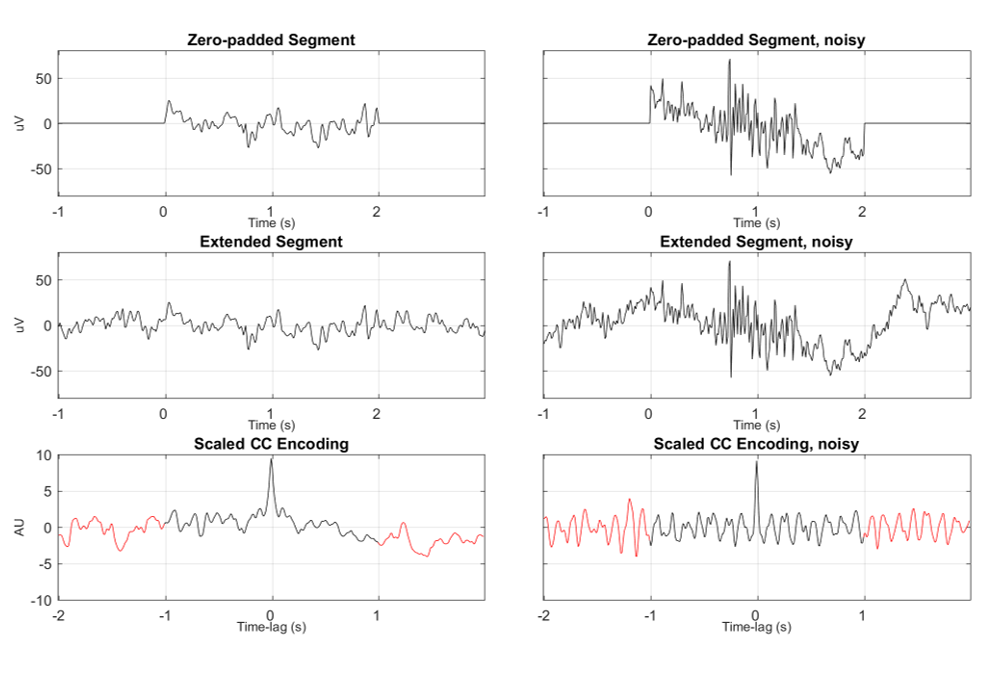
\includegraphics[width=\textwidth]{figures/paper-iii/SuppFigure_5.png}
    \caption{}
    \label{fig:paperiii-suppfigure05}
\end{figure}

Frequency content with a time resolution may also be expressed using time-frequency decompositions, such as spectrograms or scalograms, however, one of the key properties of a CNN is the ability to detect distinct features anywhere in an input, given its property of equivariance62. A CC function reveals an underlying set of frequencies as an oscillation pattern, as opposed to a spectrogram, where frequencies are displayed as small streaks or spots in specific locations, corresponding to frequencies at specific times. The length and size of each CC reflects the expected frequency content and the limit of quasi-stationarity (i.e. how quickly the frequency content is expected to change).

The EOG signal reveals information about eye movements such as REMs, and to some extent EEG activity6,7. In the case of the EOG signal, the relative phase between the two channels is of great importance to determine synchronized eye movements, and hence a CC of opposite channels (i.e. either the extended or zero padded signal is replaced with the opposite channel) is also included. The slowest eye-movements happen over the course of several seconds6,7, and hence a segment length of 4 seconds was selected for the correlation functions. To maintain resolution flexibility with the EEG, an overlap of 3.75 seconds was chosen.

In the case of the EMG signal, the main concern is the signal amplitude and the temporal resolution, not the actual frequencies. As no relevant low frequency content is expected, a segment length of 0.4 seconds and an overlap of 0.25 seconds was selected.

As with the octave encoding, the data is scaled, although only within segments:
\begin{equation}
    D_i = \frac{ \gamma_{\mathbf{x}_i \mathbf{y}_i} \func{\log}{1 + \func{\max}{\left|\gamma_{\mathbf{x}_i \mathbf{y}_i}\right|}}}{\func{\max}{\left|\gamma_{\mathbf{x}_i \mathbf{y}_i}\right|}}
\end{equation}
where $D_i$ is the scaled correlation function and $\gamma_{\mathbf{x}_i \mathbf{y}_i}$ is the unscaled correlation function.

\subsubsection{Architectures of applied CNN models}
\begin{figure}[tb]
    \centering
    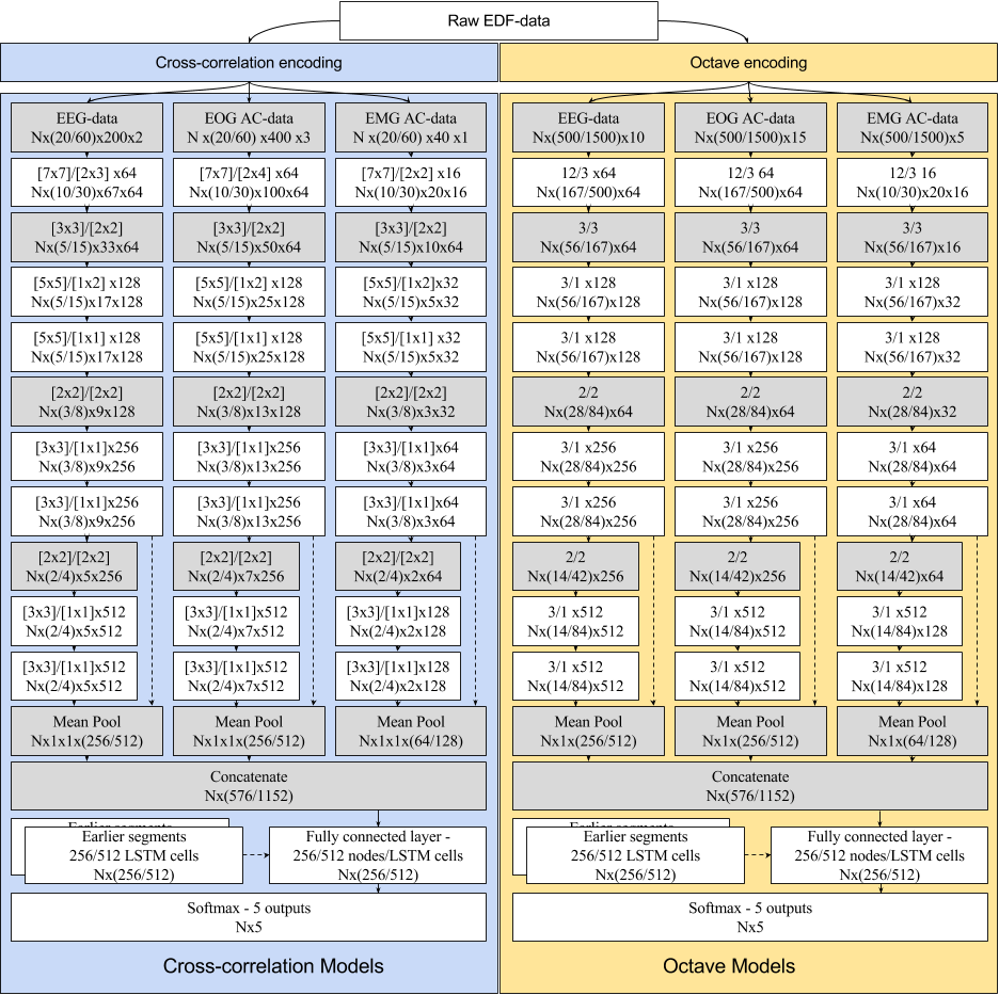
\includegraphics[width=\textwidth]{figures/paper-iii/SuppFigure_3.png}
    \caption{Caption}
    \label{fig:paperiii-suppfigure03}
\end{figure}
The architecture of a CNN typically reflects the complexity of the problem that is being solved and how much training data is available, as a complex model has more parameters than a simple model, and is therefore more likely to over-fit. However, much of this may be solved using proper regularization. Another restriction is the resources required to train a model—deep and complex models require far more operations and will therefore take longer to train and operate. In this study, no exhaustive hyper-parameter optimization was carried out. The applied architectures were chosen on the basis of other published models63. Since the models utilized three separate modalities (EEG, EOG and EMG), three separate sub-networks were constructed. These were followed by fully connected layers combining the inputs from each sub-network, which were passed onto a softmax output (Figure 6 b, Supplementary Figure 3). Models that utilize memory have fully connected hidden units replaced with LSTM cells and recurrent connections added between successive segments. Networks of two different sizes are evaluated to quantify the effect of increasing complexity. 

\subsubsection{Training of CNN models}
Training the models involves optimizing parameters to minimize a loss function evaluated across a training dataset. The loss function was defined as the cross-entropy with L2 regularization:
\begin{align}
\begin{split}
    L(\boldsymbol{\omega}) &= \frac{1}{N}\sum_{i=1}^{N} \func{H}{\mathbf{y}_i, \hat{\mathbf{y}}_i} + \ell_2 \\
    &= \frac{1}{N}_{i=1}^{N} \mathbf{y}_i \func{\log}{\hat{\mathbf{y}}_i} + \left( 1 - \mathbf{y}_i \right) \func{\log}{1 - \hat{\mathbf{y}}_i} + \lambda \| \boldsymbol{\omega} \|^2_2,
\end{split}
\end{align}
where $\mathbf{y}_i$ is the true class label of the \textit{i}th window, $\hat{\mathbf{y}}_i$ is the estimated probability of the \textit{i}th window, $\omega$ is the parameter to be updated, and $\lambda$ is the weight decay parameter set at $10^{-5}$. The model parameters were initialized with $\func{\mathcal{N}}{0, 0.01}$, and trained until convergence using stochastic gradient decent with momentum64. Weight updates were done as: $\boldsymbol{\omega}_{t+1} = \boldsymbol{\omega}_t + \eta \mathbf{v}_{t+1}$ with $\mathbf{v}_{t+1} = \alpha \mathbf{v}_t - \frac{\partial \mathbf{L}}{\partial \boldsymbol{\omega}_t}$, where $\alpha$ is the momentum set at 0.9, $\mathbf{v}_t$ is the learning velocity initialized at 0, and $\eta$ is the learning rate, initially set at 0.005. The learning rate was gradually reduced with an exponential decay $\eta = \eta_0 \exp^{-t/\tau}$, where $t$ is the number of updates and $\tau$ is a time constant, here set to 12.000.

Over-fitting was avoided using a number of regularization techniques, including batch normalization65, weight decay66, and early stopping67. Early stopping is accomplished by scheduling validation after every 50th training batch. This is done by setting aside 10\% of the training data. Training is stopped if the validation accuracy starts to decrease, as a sign of over-fitting. For LSTM networks, dropout68 was included, set at 0.5 while training. This ensured that model parameters generalized to the validation data and beyond. During training, data-batches were selected at random. Given the stochastic nature of the training procedure, it was likely that two realizations of the same model would not lead to the same results, since models end up in different local minima. To measure the effect of this, two realizations were made of each model.

Apart from model realizations, we also investigated the effect of ensembling our sleep stage classification model. In general, ensemble models can yield higher predictive performance than any single model by attacking a classification or regression problem from multiple angles. For our specific use case, this resolves into forming a sleep stage prediction based on the predictions of all the models in the given ensemble. We tested several ensembles containing various numbers of model architectures and data encodings, as described in Supplementary Table 8. 

\subsubsection{Performance comparisons of generated CNN models}
As stated, the influences of many different factors were analyzed. These included: using octave or CC encoding, short (5 s) or long (15 s) segment lengths, low or high complexity, with or without LSTM, and using a single or two realizations of a model. To quantify the effect of each, a $2^5$-factorial experiment was designed. This lead to 32 different models, see~\cref{tab:paperiii-supptable08}. Comparison between models was done on a per epoch basis. 
\begin{table}[tb]
    \centering
    \small
    \caption[STAGES models]{STAGES model tested. 32 single models are tested, and 9 ensembles, totaling 41 models.}
    \label{tab:paperiii-supptable08}
    \begin{tabular}{@{}lllll@{}}
        \toprule
        \multicolumn{5}{c}{Single models} \\ \midrule
        Memory        & Seg. Len. & Complexity & Encoding & Realizations \\
        Simple FF     & 5 s       & Low        & Octave   & 1            \\
        LSTM          & 15 s      & High       & CC       & 2            \\ \bottomrule
    \end{tabular}
    \\
    \small
    \begin{tabular}{@{}llllllllll@{}}
        \toprule
        \multicolumn{10}{c}{Ensembles} \\ \midrule
        Parameters included & All Oct FF & All Oct LSTM & All CC FF & All CC LSTM & All FF & All LSTM & All Oct models & All CC models & All models \\
        N. models           & 8          & 8            & 8         & 8           & 16     & 16       & 16             & 16            & 32         \\ \bottomrule
    \end{tabular}
\end{table}

\subsection{Results}
\subsubsection{Inter-scorer reliability cohort}

\Cref{tab:paperiii-table01} reports on the description of the various cohorts included in this study, and how they were utilized (see Datasets section in Methods).
These originate from seven different countries. 
We assessed inter-scorer reliability using the Inter-scorer Reliability Cohort (IS-RC)31, a cohort of 70 PSGs scored by 6 scorers across three locations in the United States31.
\cref{tab:paperiii-table01} displays individual scorer performance as well as the averaged performance across scorers, with top and bottom of table showing accuracies and \cohen, respectively.
The results are shown for each individual scorer when compared to the consensus of all scorers (biased) and compared to the consensus of the remaining scorers (unbiased).
In the event of no majority vote for an epoch, the epoch was counted equally in all classes in which there was disagreement.
Also shown in~\cref{tab:paperiii-table01} is the model performance on the same consensus scorings as each individual scorer along with the \textit{t}-statistic and associated \textit{p}-value for each paired \textit{t}-test between the model performance and individual scorer performance. 
At a significance level of 5\%, the model performs statistically better than any individual scorer both in terms of accuracy and \cohen.

Supplementary Table 2 displays the confusion matrix for every epoch of every scorer of the inter-scorer reliability data, both unadjusted (top) and adjusted (bottom).
As in Rosenberg and Van Hout16, the biggest discrepancies occur between N1 and Wake, N1 and N2, and N2 and N3, with some errors also occurring between N1 and REM, and N2 and REM.

For future analyses of the IS-RC in combination with other cohorts that have been scored only by one scorer, a final hypnogram consensus was built for this cohort based on the majority vote weighted by the degree of consensus from each voter, expressed as its 
\begin{equation}
    \cohen = 1 + \frac{1 - p_o}{1 - p_e},
\end{equation}
where $p_e$ is the baseline accuracy and $p_o$ is the scorer accuracy, such that
\begin{equation}
    \mathbf{y} = \argmax \frac{\sum_{i=1}^{6} \hat{\mathbf{y}}_i \cdot \boldsymbol{\kappa}_i}{\sum_{i=1}^{6} \boldsymbol{\kappa}_i}
\end{equation}
In this implementation, scorers with a higher consensus with the group are considered more reliable and have their assessments weighted heavier than the rest.
This also avoided split decisions on end-results.
\begin{table}
    \centering
    \caption{Performance of best models, as they are described by supplementary table 2, on various data-sets compared to the six-scorer consensus. All comparisons are on a by-epoch-basis.}
    \label{tab:paperiii-table02}
    \small
    \begin{tabular}{@{}lllll@{}}
        \toprule
        Test Data          & Best Single Model & Acc., \% & Best Ensemble & Acc., \% \\ \midrule
        WSC                & CC/SH/LS/LSTM/2   & $86.0 \pm 5.0$       & All CC        & $86.4 \pm 5.2$       \\
        SSC+KHC & & & & \\
        \quad $\div$ narcolepsy            & CC/LH/SS/LSTM     & $76.9 \pm 11.1$      & All CC        & $77.0 \pm 11.9$      \\
        \quad $+$ narcolepsy & CC/LH/SS/LSTM     & $68.8 \pm 11.0$      & All CC        & $68.4 \pm 12.2$      \\
        IS-RC              & CC/LH/LS/LSTM/2   & $84.6 \pm 4.6$       & All Models    & $86.8 \pm 4.3$       \\ \bottomrule
    \end{tabular}
\end{table}

\begin{landscape}
\begin{table}
    \centering
    \caption[Scorer and model performance]{Individual and overall scorer performance, expressed as accuracy (upper half) and \cohen (lower half). Both accuracy and \cohen are presented with (biased) and without (unbiased) the assessed scorer included in the consensus standard in a leave-one-out fashion. Accuracy is expressed in percent, and \cohen is a ratio and therefore unitless. \textit{t}-statistics and \textit{p}-values correspond to the paired \textit{t}-test between the unbiased predictions for each scorer against the model predictions on the same consensus.}
    \label{tab:paperiii-table01}
    \begin{tabular}{@{}llllllll@{}}
        \toprule
                                           & Overall      & Scorer 1               & Scorer 2               & Scorer 3                & Scorer 4              & Scorer 5               & Scorer 6                \\ \midrule
        Accuracy, \%                       &              &                        &                        &                         &                       &                        &                         \\
        \quad Biased                       & $81.3\pm3.0$ & $82.4\pm6.1$           & $84.6\pm5.5$           & $74.1\pm7.9$            & $85.4\pm5.7$          & $83.1\pm9.4$           & $78.3\pm8.9$            \\
        \quad Unbiased                     & $76.0\pm3.2$ & $77.3\pm6.3$           & $79.1\pm6.3$           & $69.0\pm8.0$            & $79.7\pm6.5$          & $77.8\pm9.6$           & $72.9\pm9.2$            \\
        \quad Model, \%                    & -            & $85.1\pm4.9$           & $83.8\pm5.0$           & $86.5\pm4.3$            & $84.3\pm4.7$          & $85.6\pm4.7$           & $87.0\pm4.5$            \\
        \textit{t}-stat (\textit{p}-value) & -            & $9.5$ ($3.8 \times 10^{-14}$) & $6.6$ ($7.5\times 10^{-9}$)  & $18.3$ ($6.0\times10^{-28}$) & $6.7$ ($4.7\times10^{-9}$) & $6.4$ ($1.7\times10^{-8}$)  & $12.2$ ($7.5\times10^{-19}$) \\ \midrule
        \cohen                             &              &                        &                        &                         &                       &                        &                         \\
        \quad Biased                       & $61.0\pm6.8$ & $63.6\pm12.2$          & $68.4\pm10.5$          & $45.6\pm19.7$           & $69.6\pm13.2$         & $64.5\pm20.9$          & $54.5\pm19.8$           \\
        \quad Unbiased                     & $57.7\pm6.1$ & $61.3\pm11.2$          & $64.6\pm10.3$          & $43.5\pm19.2$           & $64.6\pm13.1$         & $60.9\pm16.9$          & $51.6\pm16.7$           \\
        \quad Model                        & -            & $74.3\pm12.3$          & $72.4\pm12.1$          & $76.0\pm11.8$           & $72.7\pm12.0$         & $74.7\pm12.1$          & $76.6\pm12.2$           \\
        \textit{t}-stat (\textit{p}-value) & -            & $9.5$ ($4.6\times10^{-14}$) & $7.1$ ($7.9\times10^{-10}$) & $15.4$ ($7.0\times10^{-24}$) & $6.6$ ($6.4\times10^{-9}$) & $7.1$ ($9.2\times10^{-10}$) & $13.2$ ($2.0\times10^{-20}$) \\ \bottomrule
    \end{tabular}
\end{table}
\end{landscape}

\begin{figure}
    \centering
    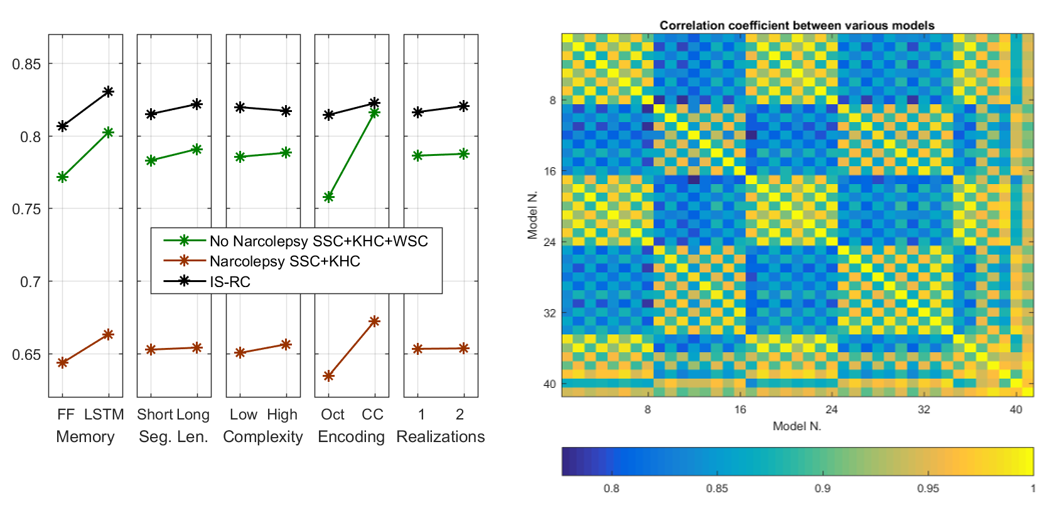
\includegraphics[width=\textwidth]{figures/paper-iii/SuppFigure_1.png}
    \caption[Comparisons of machine learning models]{Comparisons of machine learning models. Left: Comparisons of the effect on accuracy by each factor at different settings on IS-RC data, SSC and KHC narcolepsy subjects, and the remaining SSC, KHC and WSC subjects used for testing. Right: Correlation matrix showing similarities in different model predictions, where 0 means signals are independent, and 1 means signals are completely correlated. Models 1-32 are single models, and 33-41 are ensembles. The models vary on 5 parameters, each at two levels, in the following order: Memory – FF or LSTM(1), segment size – 5 s or 15 s (2), complexity – high or low (3), encoding – CC or octave (4), realizations – 1 or 2 (5). Ensembles are as described in supplementary Table 2: All FF octave models (33), all LSTM octave models (34), all FF CC models (35), all LSTM CC models (36), all FF models (37), all LSTM models (38), all CC models (39), all octave models (40), all models (41).}
    \label{fig:paperiii-suppfigure01}
\end{figure}
\subsubsection{Optimizing machine learning performance for sleep staging}
We next explored how various machine learning algorithms (see Methods) performed depending on cohort, memory (i.e., feed forward (FF) versus long short-term memory networks (LSTM)), signal segment length (short segments of 5 s (SS) versus long segments of 15 s (LS)), complexity (i.e., low (SH) vs. high (LH)), encoding (i.e., octave versus cross-correlation (CC) encoding, and realization type (repeated training sessions).
The performance of these machine learning algorithms was compared with the six-scorer consensus in the IS-RC and with single scorer data in 3 other cohorts, the Stanford Sleep Cohort (SSC)10,32, the Wisconsin Sleep Cohort (WSC)32,33 and the Korean Hypersomnia Cohort (KHC)10,34 (see Datasets section in Methods for description of each cohort).

Model accuracy varies across datasets, reflecting the fact scorer performance may be different across sites, and because unusual subjects such as those with specific pathologies can be more difficult to score—a problem affecting both human and machine scoring. 
In this study, the worst performance was seen in the KHC and SSC with narcolepsy, and the best performance was achieved on IS-RC data (\cref{fig:paperiii-suppfigure01}a,~\cref{tab:paperiii-table02}, Supplementary Table 7).
The SSC+KHC cohorts mainly contain patients with more fragmented sleeping patterns, which would explain a reduced performance. 
The IS-RC has the most accurate label, minimizing the effects of erroneous scoring, which therefore leads to an increased performance.
Incorporating large ensembles of different models increased mean performance slightly (\cref{tab:paperiii-table02}).
\begin{figure}
    \centering
    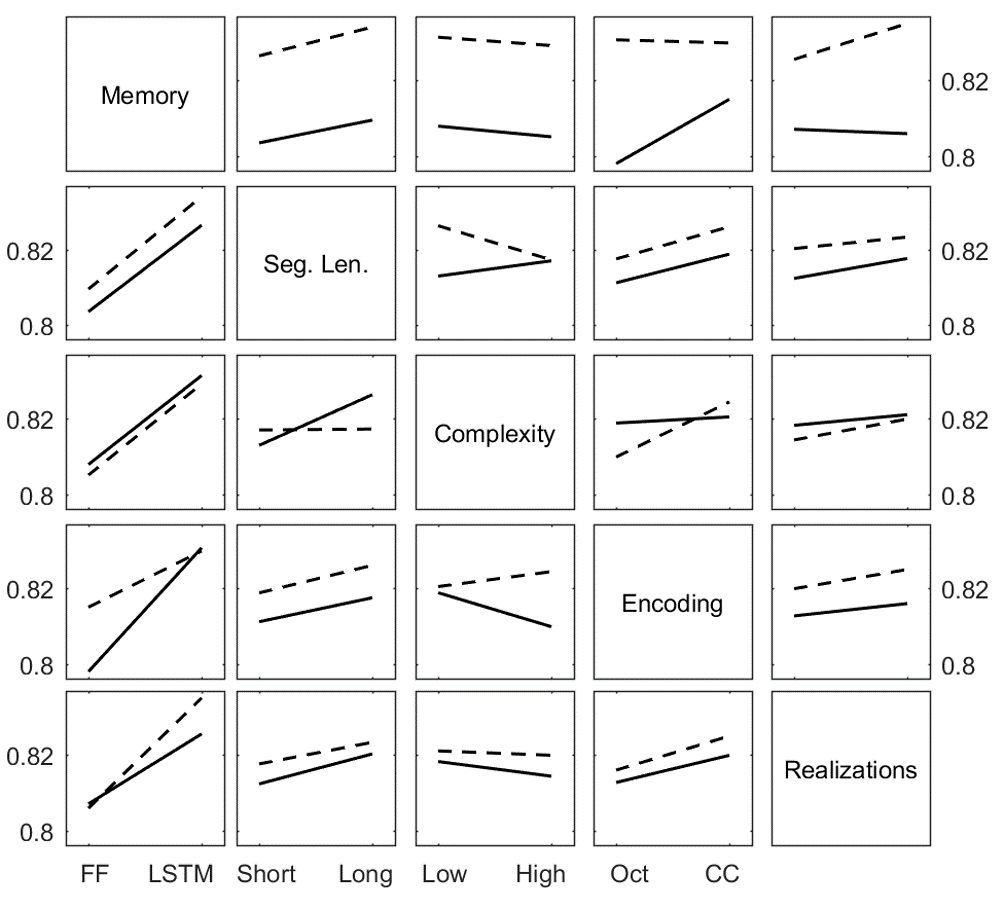
\includegraphics[width=\textwidth]{figures/paper-iii/SuppFigure_2.png}
    \caption[Interaction of different factors and their dependence on accuracy.]{Interaction of different factors and their dependence on accuracy. The IS-RC data was used for this analysis. The solid and dashed lines indicate factors along the rows on levels 1 and 2, respectively.}
    \label{fig:paperiii-suppfigure02}
\end{figure}
The two most important factors that increased prediction accuracy were encoding and memory, while segment length, complexity and number of realizations were less important (\cref{fig:paperiii-suppfigure01}).
The effect of encoding was less prominent in the IS-RC.
Prominent factor interactions include (Supplementary Figure 2): (i) CC encoding models improve with higher complexity, whereas octave encoding models worsen; (ii) increasing segment length positively affects models with low complexity, but does not affect models with a high complexity; and (iii) adding memory improves models with an octave encoding more than models with a CC encoding.
Because the ISRC data are considered the most reliable, we decided to use these data as benchmark for model comparison.
This standard improved as more scorers were added, and the model performance increased (~\cref{fig:paperiii-figure01}a).
The different model configurations described in this section do not represent exhaustive configuration search, and future work experiments might result in improved results.

Figure 2a displays typical scoring outputs (bottom panels) obtained with a single sleep study of the IS-RC cohort in comparison to 6 scorer consensus (top panel).
The model results are displayed as hypnodensity graphs, representing not only discrete sleep stage outputs, but also the probability of occurrence of each sleep state for each epoch (see definition in Data labels, scoring and fuzzy logic section).
As can be seen, all models performed well, and segments of the sleep study with the lowest scorer consensus (top) are paralleled by similar sleep stage probability uncertainty, with performance closest to scoring consensus achieved by an ensemble model described below (second to top).

\subsubsection{Final implementation of automatic sleep scoring algorithm}
Because of model noise, potential inaccuracies and the desire to quantify uncertainty, the final implementation of our sleep
scoring algorithm is an ensemble of different CC models with
small variations in model parameters, such as the number of
feature-maps and hidden nodes.
This was achieved by randomly varying the parameters between 50 and 150\% of the original values using the CC/SH/LS/LSTM as a template (this model achieved similar performance to the CC/LH/LS/LSTM while requiring significantly less computational power).
\begin{table}[]
    \centering
    \caption[STAGES model confusion matrix]{Confusion matrix displaying the relation between different targets and the ensemble estimate. The targets are: Top row – un-weighted consensus. Bottom row – weighted by the scorer agreement at each epoch. The number of analyzed epochs were 53009 (un-weighted) and 36032 (weighted).}
    \label{tab:paperiii-table03}
    \begin{tabular}{@{}llcccccc@{}}
        \toprule
                                           &        & \multicolumn{5}{c}{Target}                    & \multicolumn{1}{l}{} \\ \cline{3-7}
                                           &  & Wake    & N1     & N2      & N3     & REM     & Precision            \\ \midrule
        \multirow{10}{*}{\rotatebox[origin=c]{90}{Model prediction}} & Wake   & 14.08\% & 0.35\% & 0.88\%  & 0.01\% & 0.08\%  & 0.91                 \\
                                           &        & 16.68\% & 0.15\% & 0.44\%  & 0.00\% & 0.02\%  & 0.96                 \\
                                           & N1     & 1.13\%  & 1.78\% & 3.00\%  & 0.00\% & 0.36\%  & 0.28                 \\
                                           &        & 0.47\%  & 0.88\% & 1.15\%  & 0\%    & 0.12\%  & 0.34                 \\
                                           & N2     & 0.29\%  & 0.59\% & 52.58\% & 1.27\% & 0.66\%  & 0.95                 \\
                                           &        & 0.12\%  & 0.25\% & 56.30\% & 0.34\% & 0.32\%  & 0.98                 \\
                                           & N3     & 0.00\%  & 0\%    & 2.13\%  & 4.87\% & 0\%     & 0.7                  \\
                                           &        & 0\%     & 0\%    & 1.09\%  & 4.23\% & 0\%     & 0.91                 \\
                                           & REM    & 0.54\%  & 1.17\% & 0.78\%  & 0\%    & 13.45\% & 0.84                 \\
                                           &        & 0.40\%  & 0.73\% & 0.41\%  & 0\%    & 15.86\% & 0.91                 \\
                                           & Sensitivity       & 0.88    & 0.46   & 0.89    & 0.79   & 0.92    & 0.87                 \\
                                           &        & 0.94    & 0.44   & 0.95    & 0.92   & 0.97    & 0.94                 \\ \bottomrule
    \end{tabular}
\end{table}
All models make errors, but as these errors occur independently of each other, the risk of not detecting and correcting errors falls with increasing model numbers.
For this reason, 16 such models were trained, and at each analyzed segment both mean and variance of model estimates were calculated. 
As expected, the relative model variance (standardized to the average variance in a correct wakefulness prediction) is generally lower in correct predictions (Supplementary Table 3) and this can be used to inform users about uncertain/incorrect estimates. 
To demonstrate the effectiveness of this final implementation, the average of the models is shown alongside the distribution of \plusminus{5234}{14} scorers on 150 epochs, a dataset provided by the AASM (AASM inter-scorer reliability (ISR) dataset, (see Datasets section in Methods). 
On these epochs, the AASM ISR achieved a 90\% agreement between scorers. 
In comparison, the model estimates reached a 95\% accuracy compared to the AASM consensus (Fig. 2b). 
Using the model ensemble and reporting on sleep stage probabilities and inter-model variance for quality purpose constitute the core of our sleep scoring algorithm.
\begin{figure}[tbh]
    \centering
    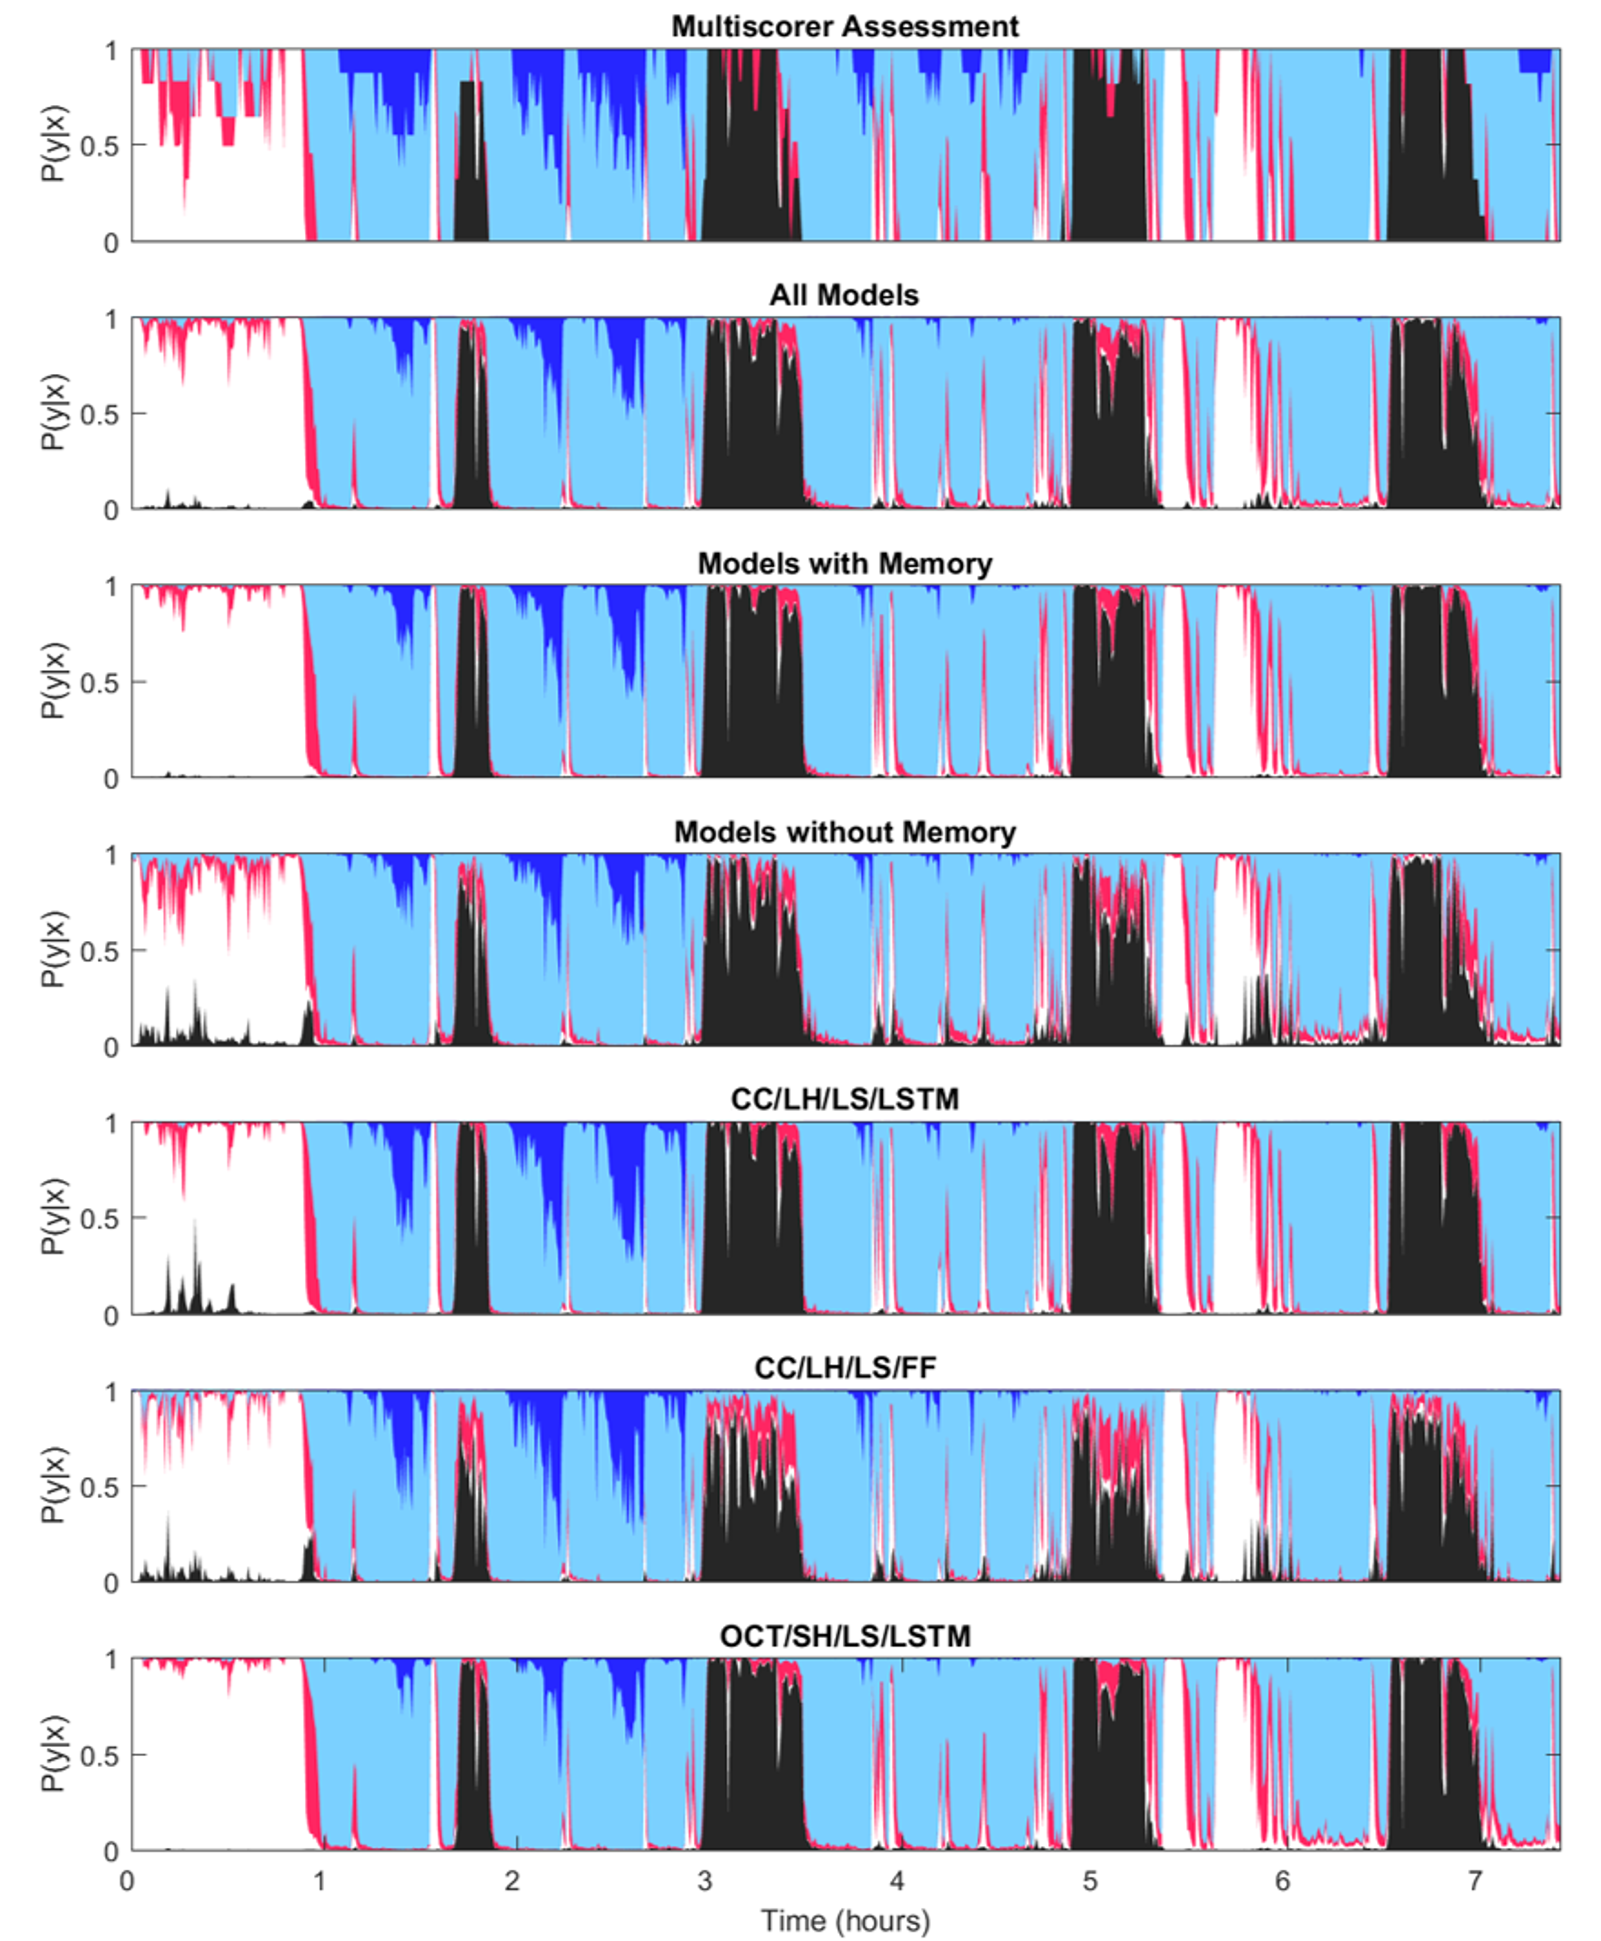
\includegraphics[width=\textwidth]{figures/paper-iii/Figure_2a}
    \caption{The figure displays the hypnodensity graph. Displayed models are, in order: multiple scorer assessment (1); ensembles as described in Supplementary Table 8: All models, those with memory (LSTM) and those without memory (FF) (2–4); single models, as described in Supplementary Table 8 (5–7). OCT is octave encoding, Color codes: white, wake; red, N1; light blue, N2; dark blue, N3; black, REM.}
    \label{fig:paperiii-figure02a}
\end{figure}
\begin{figure}[htb]
    \centering
    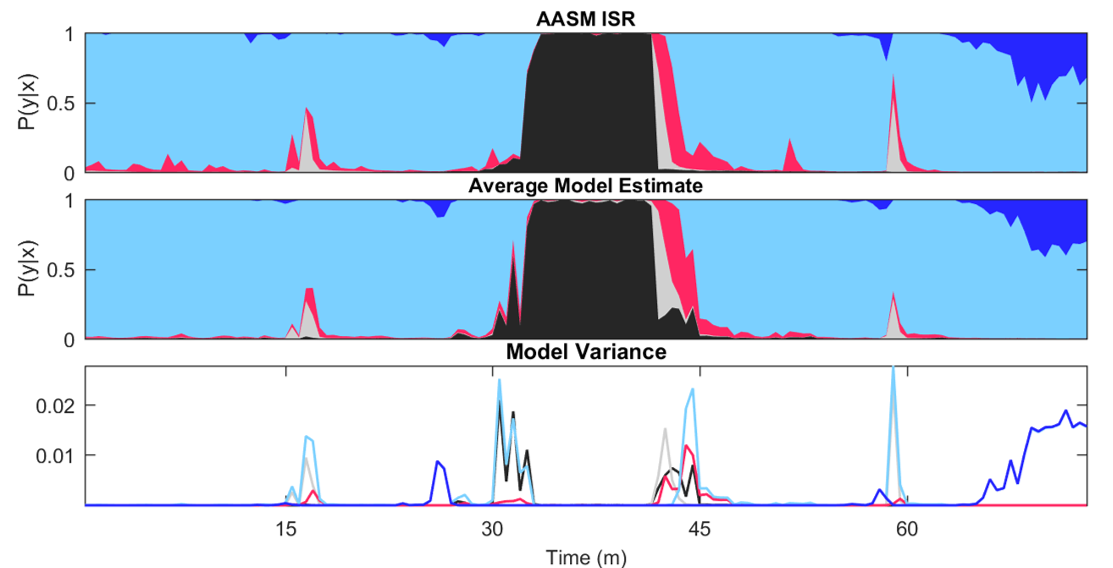
\includegraphics[width=\textwidth]{figures/paper-iii/Figure_2b}
    \caption{The 150 epochs of a recording from the AASM ISR program are analyzed by 16 models with randomly varying parameters, using the CC/SH/LS/LSTM model as a template. These data were also evaluated by \plusminus{5234}{14} different scorers. The distribution of these is shown on top, the average model predictions are shown in the middle, and the model variance is shown at the bottom.}
    \label{fig:paperiii-figure02b}
\end{figure}
\subsubsection{Ensemble/best model performance}
Supplementary Table 2 reports on concordance for our best model, the ensemble of all CC models.
Concordance is presented in a weighted and unweighted manner, between the best model estimate and scorer consensus (\cref{tab:paperiii-table03}).
Weighing of a segment was based on scorer confidence and serves to weigh down controversial segments.
For each recording \textit{i}, the epoch-specific weight $w_n$ and weighted accuracy $\alpha w$ were calculated as:
\begin{align}
\begin{split}
    w_n &= \func{\max_{z \in \mathcal{Z}}}{\func{\mathbf{P}}{\mathbf{y}_n | \mathbf{x}_n}} - \func{\ell_{\mathcal{Z}}^2}{\func{\mathbf{P}}{\mathbf{y}_n | \mathbf{x}_n}}, \\
    \alpha_w^{(i)} &= \frac{1}{\sum_n w_n} \sum_n w_n \! \left( \func{\argmax_{m \in \mathcal{M}}}{\func{\mathbf{P}_m}{\hat{\mathbf{y}}_n | \mathbf{x}_n}} \cap \func{\argmax_{z \in \mathcal{Z}}}{\func{\mathbf{P}_z}{\mathbf{y}_n | \mathbf{x}_n}} \right),
\end{split}
\end{align}
where $\func{\ell_{\mathcal{Z}}^2}{\func{\mathbf{P}}{\mathbf{y}_n | \mathbf{x}_n}}$ is the second most likely stage assessed by the set of scorers (experts) denoted by $\mathcal{Z}$, of the \textit{n}th epoch in a sleep recording.
As with scorers, the biggest discrepancies occurred between wake versus N1, N1 versus N2 and N2 versus N3.
Additionally, the weighted performance was almost universally better than the unweighted performance, raising overall accuracy from 87 to 94\%, indicating a high consensus between automatic scoring and scorers in places with high scorer confidence.
An explanation for these results could be that both scorers and model are forced to make a choice between two stages when data are ambiguous.
An example of this may be seen in Fig. 2a.
Between 1 and 3 h, several bouts of N3 occur, although they often do not reach the threshold for being the most likely stage
As time progresses, more evidence for N3 appears reflecting increased proportion of slow waves per epoch, and confidence increases, which finally yields “definitive” N3. 
This is seen in both model and scorer estimates.
Choosing to present the data as hypnodensity graphs mitigates this problem. 
The various model estimates produce similar results, which also resemble the scorer assessment distribution, although models without memory fluctuate slightly more, and tend to place a higher probability on REM sleep in periods of wakefulness, since no contextual information is provided

% \begin{figure}[!tb]
%     \myfloatalign   
%     \subfloat[]
%     {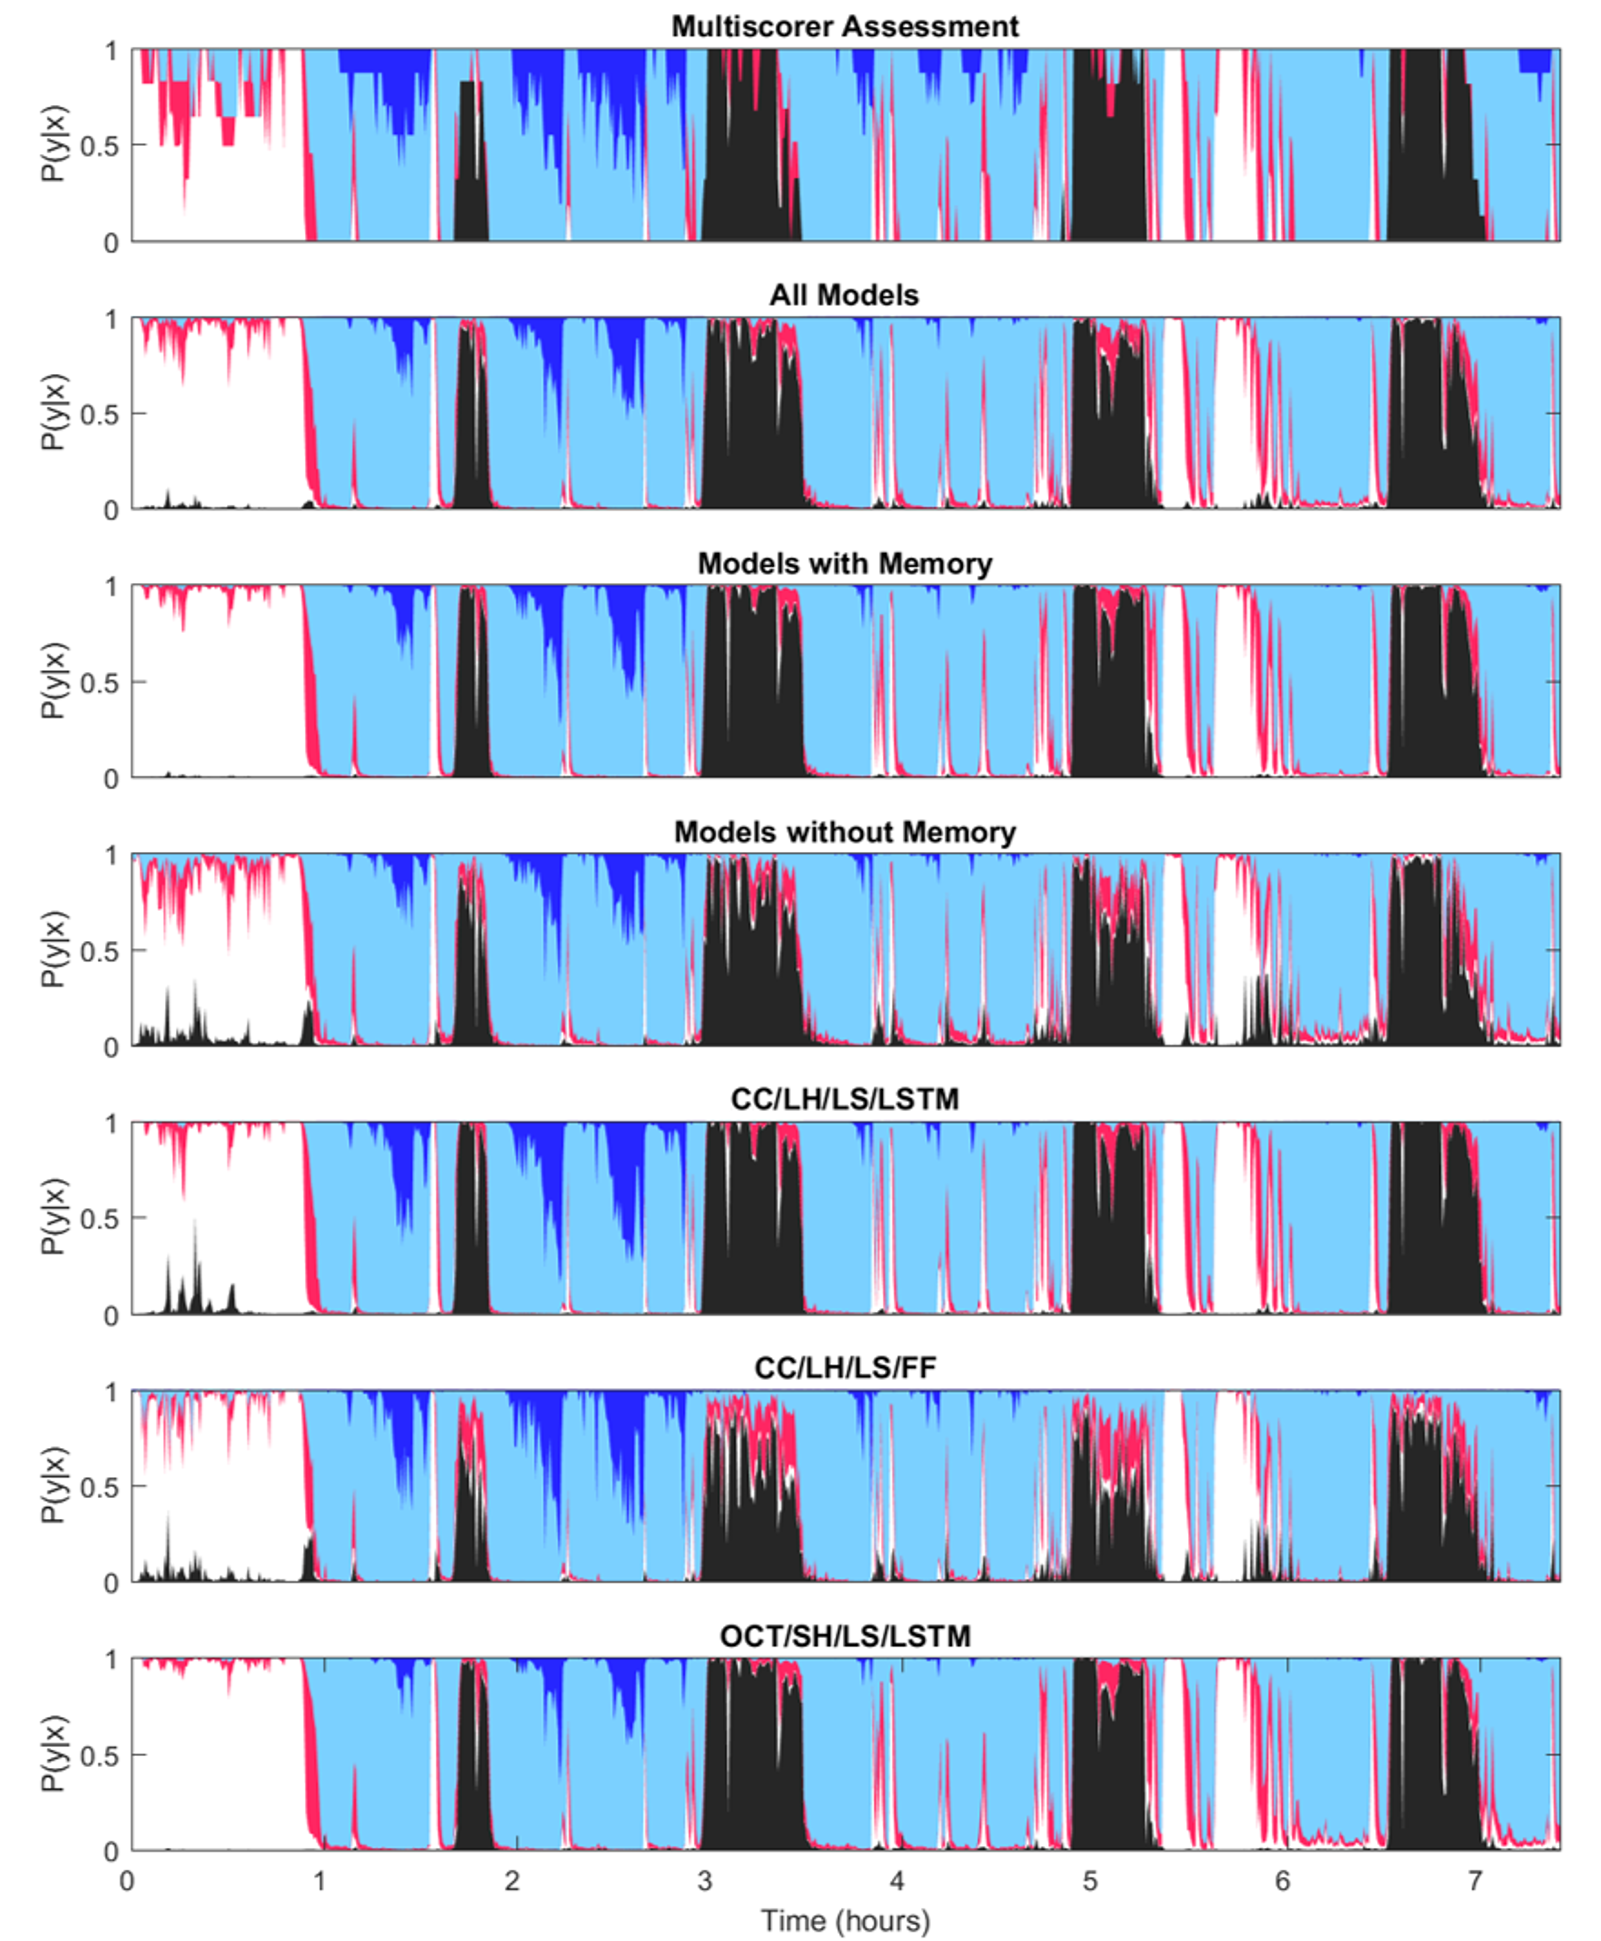
\includegraphics[width=\textwidth]{figures/paper-iii/Figure_2a}} \\
%     \subfloat[]
%     {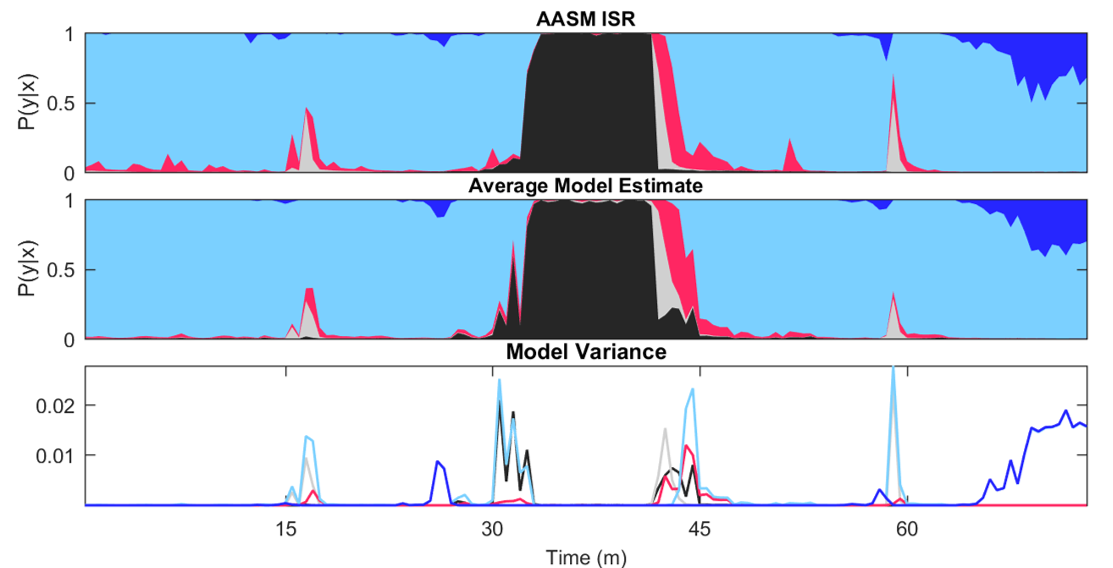
\includegraphics[width=\textwidth]{figures/paper-iii/Figure_2b}}
%     \caption[Hypnodensity example evaluated by multiple scorers and different predictive models]{Hypnodensity example evaluated by multiple scorers and different predictive models. (a)  b }
%     \label{fig:paperiii-figure02}
% \end{figure}

\subsubsection{Influences of sleep pathologies}
As seen in Table 2, the different cohorts achieve different performances.
To see how much may be attributed to various pathologies, five different analyses of variance were made, with accuracy as the dependent variable, using cohort, age (grouped as age $<$ 30, 30 $\leq$ age $<$ 50, and age $\geq$ 50) and sex as covariates (Supplementary Table 4), investigating the effect of insomnia, OSA, restless leg syndrome (RLS), periodic leg movement index (PLMI) and T1N on accuracy of our machine learning routine versus human scoring. 
This was performed in the cohort mentioned above with addition of the Austrian Hypersomnia Cohort (AHC)35. 
The \textit{p}-values obtained from paired \textit{t}-testing for each condition were $0.75$ (insomnia), $7.53 \times 10^{-4}$ (OSA), $0.13$ (RLS), $0.22$ (PLMI) and $1.77 \times 10^{-15}$ (T1N) respectively, indicating that only narcolepsy had a strong effect on scorer performance. 
Additionally, in the context of narcolepsy, cohort and age yielded \textit{p}-values between $3.69 \times 10^{-21}$ and $2.81 \times 10^{-82}$ and between $0.62$ and $6.73 \times 10^{-6}$, respectively. 
No significant effect of gender was ever noted. 
Cohort effects were expected and likely reflect local scorer performances and differences in PSG hardware and filter setups at every site. 
Decreased performance with age likely reflects decreased EEG amplitude, notably in N3/slow wave sleep amplitude with age36.

\begin{figure}[tb]
    \myfloatalign   
    \subfloat[]
    {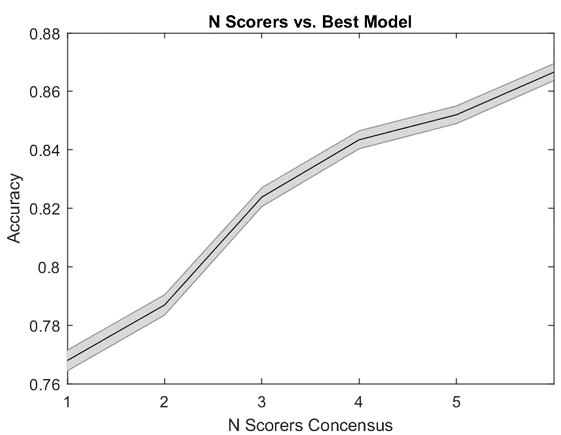
\includegraphics[width=0.48\textwidth]{figures/paper-iii/Figure_1a}}  ~
    \subfloat[]
    {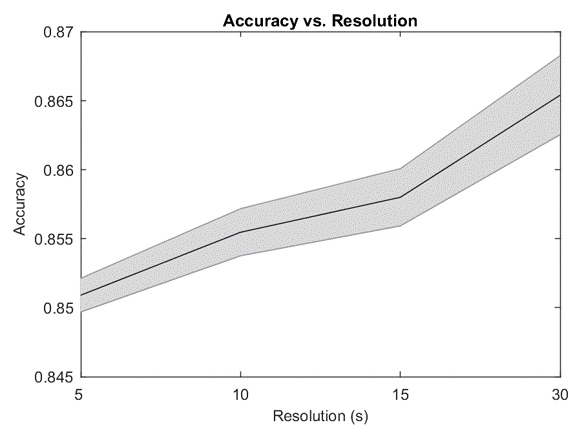
\includegraphics[width=0.5 \textwidth]{figures/paper-iii/Figure_1b}}
    \caption[Accuracy per scorer and by time resolution]{Accuracy per scorer and by time resolution. (a) The effect on scoring accuracy as golden standard is improved. Every combination of $N$ scorers is evaluated in an unweighted manner and the mean is calculated. Accuracy is shown with mean (solid black line) and a 95\% confidence interval (gray area). (b) Predictive performance of best model at different resolutions. Performance is shown as mean accuracy (solid black line) with a 95\% confidence interval
(gray area).}
    \label{fig:paperiii-figure01}
\end{figure}
\subsubsection{Resolution of sleep stage scoring}
Epochs are evaluated with a resolution of 30 s, a historical standard that is not founded in anything physiological, and limits the analytical possibilities of a hypnogram.
Consequently, it was examined to what extent the performance would change as a function of smaller resolution.
Only the models using a segment size of 5 s were considered.
Segments were averaged to achieve performances at 5, 10, 15 and 30 s resolutions, and the resulting performances in terms of accuracy are shown in~\cref{fig:paperiii-figure01}b. 
Although the highest performance was found using a resolution of 30 s, performance dropped only slightly with decreasing window sizes.

\subsection{Discussion}
In recent years, machine learning has been used to solve similar or more complex problems, such as labeling images, understanding speech and translating language, and have seen advancement to the point where humans are now sometimes outperformed21–23, while also showing promising results in various medical fields24–29.
Automatic classification of sleep stages using automatic algorithms is not novel44,45, but only recently has this type of machine learning been applied and the effectiveness has only been demonstrated in a small numbers of sleep studies46–49. 
Because PSGs contain large amounts of manually annotated “gold standard” data, we hypothesized this method would be ideal to
automatize sleep scoring.
We have shown that machine learning can be used to score sleep stages in PSGs with high accuracy in multiple physical locations in various recording environments, using different protocols and hardware/software configurations, and in subjects with and without various sleep disorders.

After testing various machine learning algorithms with and without memory and specific encodings, we found increased robustness using a consensus of multiple algorithms in our prediction.
The main reason for this is likely the sensitivity of each algorithm to particular aspects of each individual recording, resulting in increased or decreased predictability.
\Cref{fig:paperiii-suppfigure01}b displays the correlations between different models.
Models that incorporate an ensemble of different models generally have a higher overall correlation coefficient than singular models, and since individual models achieve similar performances, it stands to reason that these would achieve the highest performance.

One potential source for this variability was, in addition to the stochastic nature of the training, the fact recordings were conducted in different laboratories that were using different hardware and filters, and had PSGs scored by technicians of various abilities.
Another contributor was the presence of sleep pathologies in the dataset that could influence machine learning.
Of the pathologies tested, only narcolepsy had a very significant effect on the correspondence between manual and machine learning methods ($p=1.77 \times 10^{-15}$ vs $p=7.53 \times 10^{-4}$ for sleep apnea for example, see Supplementary Tables 4 and 7).
This was not surprising as the pathology is characterized by unusual sleep stage transitions, for example, transitions from wake to REM sleep, which may make human or machine learning staging more difficult.
This result suggests that reporting inter-model variations in accuracy for each specific patient has value in flagging unusual sleep pathologies, so this metric is also reported by our detector.

Unlike previous attempts using automatic detector validations, we were able to include 70 subjects scored by 6 technicians in different laboratories (the IS-RC cohort)31 to independently validate our best automatic scoring consensus algorithm.
This allowed us to estimate the performance at 87\% in comparison to the performance of a consensus score for every epoch among six expert technicians (ultimate gold standard) (Table 1).
Including more scorers produces a better gold standard, and as~\cref{fig:paperiii-figure01}a indicates, the model accuracy also increases with more scorers.
Naturally, extrapolating from this should be done with caution; however, it is reasonable to assume that the accuracy would continue to increase with increased scorers.
In comparison, performance of any individual scorer ranges from 74 to 85\% when compared to the same six-scorer gold standard, keeping in mind this performance is artificially inflated since the same scorers evaluated are included in the gold standard (unbiased performance of any scorer versus consensus of remaining 5 scorers range from 69 to 80\%). 
The best model achieves 87\% accuracy using 5 scorers (~\cref{fig:paperiii-figure01}a and Table 1), and is statistically higher than all scorers.

As with human scorers, the biggest discrepancies in machine learning determination of sleep stages occurred between wake versus N1, N1 versus N2 and N2 versus N3.
This is logical as these particular sleep stage transitions are part of a continuum, artificially defined and subjective. To give an example: an epoch comprised of 18\% slow wave activity is considered N2 while an epoch comprised of 20\% slow wave activity qualifies as N3.
Overall, data indicate that our machine learning algorithm performs better than individual scorers, as typically used in clinical practice, or similar to the best of 5 scorers in comparison to a combination of 5 experts scoring each epoch by consensus.
It is also able to score at higher resolution, i.e., 5 s, making it unnecessary to score sleep stages by 30 s epochs, an outdated rule dating from the time sleep was scored on paper. 
Although the data sample used for multi-scorer validation contained only female subjects, the scoring accuracy of our model was not seen to be affected by gender (Supplementary Table 3) in another analysis.

Using our models, and considering how typical T1N behaved in our sleep stage machine learning routines, we extracted features that could be useful to diagnose this condition.
T1N ischaracterized by the loss of hypocretin-producing cells in the hypothalamus3 and can be best diagnosed by measuring hypocretin levels in the CSF11, a procedure that requires a lumbar puncture, a rarely performed procedure in the United States. 
At the symptomatic level, T1N is characterized by sleepiness, cataplexy (episodes of muscle weakness during wakefulness triggered by emotions) and numerous symptoms reflecting poor nocturnal sleep (insomnia) and symptoms of “dissociated REM sleep”.
Dissociated REM sleep is reflected by the presence of unusual states of consciousness where REM sleep is intermingled with wakefulness, producing disturbing reports of dreams that interrupt wakefulness and seem real (dream-like hallucinations), or episodes where the sleeper is awake but paralyzed as in normal REM sleep (sleep paralysis).
The current gold standard for T1N diagnosis is the presence of cataplexy and a positive MSLT.
In a recent large study of the MSLT, specificity and sensitivity for T1N was 98.6\% and 92.9\% in comparing T1N versus controls, and 71.2\% and 93.4\% in comparing T1N versus other hypersomnia cases (high pretest probability cohort)10.

Table 4 and Supplementary Table 5 reveal features found in nocturnal PSGs that discriminate type 1 narcoleptics and nonnarcoleptics.
One of the most prominent features, short latency REM sleep, bears great resemblance to the REM sleep latency, which is already used clinically to diagnose narcolepsy, although in this case it is calculated using fuzzy logic and thus represent a latency where accumulated sleep is suggestive of a high probability of REM sleep having occurred (as opposed to a discreteREM latency scored by a technician).
A short REM  latency during nocturnal PSG (typically 15 min) has recently been shown to be extremely specific (99\%) and moderately sensitive (40–50\%) for T1N10,50.
The remaining selected features also describe a generally altered sleep architecture, particularly between REM sleep,
light sleep and wake, aspects of narcolepsy already known and
thus reinforcing their validity as biomarkers.

For example, the primary feature as determined by the RFE algorithm was the time taken until 5\% of the accumulated sum of the probability products between stages W, N2 and REM had been reached (see also Table 4), which reflects the uncertainty between wakefulness, REM and N2 sleep at the beginning of the night.
Specifically, for the \textit{n}th epoch, the model will output probabilities for each sleep stage, and the proto-feature $\boldsymbol{\Phi}_n$ is calculated as
\begin{equation}
    \boldsymbol{\Phi}_n = \func{p}{\wake} \times \func{p}{\nII} + \func{p}{\wake} \times \func{p}{\rem} + \func{p}{\nII} \times \func{p}{\rem}.
\end{equation}
The feature value is then calculated as the time it takes in minutes for the accumulated sum of $\boldsymbol{\Phi}_n$ to reach 5\% of the total sum $\sum_n \boldsymbol{\Phi}_n$.
Since each of probability product in $\boldsymbol{\Phi}_n$ reflects the staging uncertainty between each sleep stage pair, $\boldsymbol{\Phi}_n$ alone reflects the general sleep stage uncertainty for that specific epoch as predicted by the model.
A very high value will be attained for epoch $n$ if the probabilities for N2, W and REM are equally probable with probabilities for the remaining sleep stages being low or close to zero. 
A PSG with a high staging uncertainty between sleep and wake early in the night would reach the 5\% threshold rapidly.

Using these features, we were able to determine an optimal cutoff that discriminated narcolepsy from controls and any other patients with as high specificity and sensitivity as the MSLT (Supplementary Table 6), notably when HLA typing is added.
This is true for both the test and the never seen replication samples.
Although we do observe a small drop in specificity in the replication sample, the efficacy of the detector was also tested in the context of naive patients with hypersomnia (high pretest probability sample), and performance found to be similar to the MSLT.

MSLT testing requires that patients spend an entire night and day in a sleep laboratory.
The use of this novel biomarker could reduce time spent to a standard 8 h night recording, as done for the screening of other sleep pathologies (e.g., OSA), allowing improved recognition of T1N cases at a fraction of the cost.
A positive predictive value could also be provided depending on the nature of the sample and known narcolepsy prevalence (low in general population screening, intermediary in overall clinic population sample and high in hypersomnia cohorts). 
It also opens the possibility of using home sleep recordings for diagnosing narcolepsy. 
In this direction, because of the probabilistic and automatic nature of our biomarker, estimates from more than one night could be automatically analyzed and combined over time, ensuring improved prediction.
However, it is important to note that this algorithm will not replace the MSLT in the ability to predict excessive daytime sleepiness through the measure of mean sleep latency across daytime naps, which is an important characteristic of other hypersomnias.

In conclusion, models which classify sleep by assigning a membership function to each of five different stages of sleep for each analyzed segment were produced, and factors contributing to the performance were analyzed. 
The models were evaluated on different cohorts, one of which contained 70 subjects scored by 6 different sleep scoring technicians, allowing for inter-scorer reliability assessments.
The most successful model, consisting of an ensemble of different models, achieved an accuracy of 87\% on this dataset, and was statistically better performing than any individual scorer.
It was also able to score sleep stages with high accuracy at lower time resolution (5 s), rendering the need for scoring per 30 s epoch obsolete.
When predictions were weighted by the scorer agreement, performance rose to 95\%, indicating a high consensus between the model and human scorers in areas of high scorer agreement.
A final implementation was made using an ensemble with small variations of the best single model.
This allowed for better predictions, while also providing a measure of uncertainty in an estimate.

When the staging data were presented as hypnodensity distributions, the model conveyed more information about the subject than through a hypnogram alone.
This led to the creation of a biomarker for narcolepsy that achieved similar performance to the current clinical gold standard, the MSLT, but only requires a single sleep study.
If increased specificity is needed, for example, in large-scale screening, HLA or additional genetic typing brings specificity above 99\% without loss of sensitivity.
This presents an option for robust, consistent, inexpensive and simpler diagnosis of subjects who may have narcolepsy, as such tests may also be carried out in a home environment.

This study shows how hypnodensity graphs can be created automatically from raw sleep study data, and how the resulting interpretable features can be used to generate a diagnosis probability for T1N.
Another approach would be to classify narcolepsy directly from the neural network by optimizing the performance not only for sleep staging, but also for direct diagnosis by adding an additional softmax output, thereby creating a multitask classifier.
This approach could lead to better predictions, since features are not then limited to by a designer imagination. 
A drawback of this approach is that features would no longer be as interpretable and meaningful to clinicians. 
If meaning could be extracted from these neural network generated features, this might open the door to a single universal sleep analysis model, covering multiple diseases.
Development of such a model would require adding more subjects with narcolepsy and other conditions to the pool of training data.

% \section{Sleep stage classification algorithms}


% Chapter summary
\clearpage\section{Chapter summary}\label{sec:sleep-stage-classification:summary}

Sleep%
\graffito{\ref{hypothesis:sleep-stages}: \hypothesis{} sleep stages} %
stage classification is performed manually by experts in sleep clinics leading to major inter- and intra-variability~\cite{Norman2000,Rosenberg2013,Younes2017,Younes2016,Younes2018}.
One potential way to overcome this challenge is to assist or augment the manual scoring with fully automatic intelligent systems (\ref{hypothesis:sleep-stages}), that provide consistency and robustness in the analysis of sleep patterns.
In this chapter, we introduced methods for automating sleep stage classification using deep neural networks with two separate model frameworks to answer research questions~\ref{question:sleep-stages-classification}, \ref{question:sleep-stages-datasets}, and \ref{question:sleep-stages-guarantee}.

\Cref{sec:paperi}\graffito{\ref{question:sleep-stages-classification}: \questionSleepStageClassification} described the initial version of the \ac{MASSC} algorithm, and end-to-end deep learning model based on the ResNet-50 architecture. 
We trained and tested the algorithm on a collective of 2310 \acp{PSG} using three different training strategies, the best of which yielded a high accuracy value of 84.1\% and a \cohen of 0.746.
In view of the large number of \ac{PSG} recordings included in the study, these numbers compare favorably to the current state-of-the-art in automatic sleep stage scoring, as well as the reported inter-rater reliability measures described in~\cref{sec:challenges-sleep-stage-scoring}.

However%
\graffito{\ref{question:sleep-stages-datasets}: \questionSleepStageDatasets}, %
like many other published papers on automatic sleep stage classification, the results reported in~\cref{sec:paperi} are based solely on a single cohort of \acp{PSG}, which immediately raises concerns over the actual generalizability of the model.
In~\cref{sec:paperii} we applied an updated version of the \ac{MASSC} algorithm in four different experimental settings using five cohorts differing in size, demographics, inherent co-morbidities and recording setups.
We found that training models on individual cohorts yielded large variations in classification performance both in \ac{LOCI} and \ac{LOCO} training configurations. 
Strikingly, we found consistently higher sleep stage classification accuracy as a function of the data fraction by mixing cohorts in the training data compared to training models on single cohorts.
Using 100\% of the training data, our model achieved an accuracy of 86.9\% and a \cohen of 0.799, which in light of the high numbers of both training and testing records compares favorably to the state-of-the-art, as well as our previous reported results in~\cref{sec:paperi}.

The%
\graffito{\ref{question:sleep-stages-guarantee}: \questionSleepStageGuarantee} %
final section described the sleep stage classification part of the \ac{STAGES} model.
Here, we used specific transformations of the input \ac{PSG} signals coupled with multiple realizations of a deep neural network architecture to create a final ensemble model for classifying sleep stages.
Based on a total 2784 \acp{PSG}, the best performing model as determined by a \(2^5\)-factorial experimental design yielded an accuracy of 86.8\% on a dataset scored by six technicians, while outperforming every single one based on both a biased and unbiased consensus score.
The model was also shown to be stable with respect to the presence of several sleep disorders, with the exception of narcolepsy which had a significant impact on the algorithm.\graffito{The implications of this will be detailed in~\cref{chap:classification-sleep-disorders}}